\documentclass[9pt]{article}
\usepackage[english]{babel}
\usepackage{amsmath,amsthm}
\usepackage{amsfonts}
\usepackage{graphicx}
\usepackage[margin=0.2in]{geometry}
\newcommand{\setlinespacing}[1]{\setlength{\baselineskip}{#1 \defbaselineskip}}
\newcommand{\doublespacing}{\setlength{\baselineskip}{2.0 \defbaselineskip}}
\newcommand{\singlespacing}{\setlength{\baselineskip}{\defbaselineskip}}
\newcommand{\A}{{\cal A}}
\newcommand{\h}{{\cal H}}
\newcommand{\s}{{\cal S}}
\newcommand{\W}{{\cal W}}
\newcommand{\BH}{\mathbf B(\cal H)}
\newcommand{\KH}{\cal  K(\cal H)}
\newcommand{\Real}{\mathbb R}
\newcommand{\Complex}{\mathbb C}
\newcommand{\Field}{\mathbb F}
\newcommand{\RPlus}{[0,\infty)}
\newcommand{\norm}[1]{\left\Vert#1\right\Vert}
\newcommand{\essnorm}[1]{\norm{#1}_{\text{\rm\normalshape ess}}}
\newcommand{\abs}[1]{\left\vert#1\right\vert}
\newcommand{\set}[1]{\left\{#1\right\}}
\newcommand{\seq}[1]{\left<#1\right>}
\newcommand{\eps}{\varepsilon}
\newcommand{\To}{\longrightarrow}
\newcommand{\RE}{\operatorname{Re}}
\newcommand{\IM}{\operatorname{Im}}
\newcommand{\Poly}{{\cal{P}}(E)}
\newcommand{\EssD}{{\cal{D}}}
\newcommand{\field}[1]{\mathbb{#1}}
\newcommand{\C}{\field{C}}
\newcommand{\R}{\field{R}}
\newcommand{\script}[1]{\mathcal{#1}}
\newcommand{\fall}{\; \forall \;}
\newcommand{\exts}{\; \exists \;}
\newcommand{\mbf}[1]{\mathbf{#1}}
\newcommand{\binomial}[2]{\biggl( \begin{array}{c}  #1 \\ #2  \\ \end{array} \biggr) }
\newcommand{\fderiv}[2]{ \frac{d}{ d #1} \: #2}
\newcommand{\sderiv}[2]{ \frac{d^2}{ d^2 #1} \: #2}
\newcommand{\pfderiv}[2]{ \frac{\partial}{ \partial #1} \: #2}
\newcommand{\psderiv}[2]{ \frac{\partial^2}{ \partial^2 #1} \: #2}
\newcommand{\mat}[1]{\mathbf{#1}}
\DeclareSymbolFont{AMSb}{U}{msb}{m}{n}
\DeclareMathSymbol{\dblz}{\mathalpha}{AMSb}{"5A}
\DeclareMathSymbol{\dblr}{\mathalpha}{AMSb}{"52}
\DeclareMathSymbol{\dblt}{\mathalpha}{AMSb}{"54}
\DeclareMathSymbol{\dblq}{\mathalpha}{AMSb}{"51}
\DeclareMathSymbol{\dbln}{\mathalpha}{AMSb}{"4E}
\DeclareMathSymbol{\dblf}{\mathalpha}{AMSb}{"46}
\DeclareMathSymbol{\dblc}{\mathalpha}{AMSb}{"43}
\DeclareMathSymbol{\dbld}{\mathalpha}{AMSb}{"44}
\theoremstyle{plain}
\newtheorem{thm}{Theorem}[section]
\newtheorem{cor}[thm]{Corollary}
\newtheorem{lem}[thm]{Lemma}
\newtheorem{prop}[thm]{Proposition}
\theoremstyle{definition}
\newtheorem{defn}{Definition}[section]
\theoremstyle{remark}
\newtheorem{rem}{Remark}[section]
\numberwithin{equation}{section}
\renewcommand{\theequation}{\thesection.\arabic{equation}}
\begin{document}
\title{Regression of KL Software Distribution   }
\author{KL Software Libraries}
\date{Thu Jun 12 01:04:36 2014
}
\maketitle
\textbf{ KL Library test output.  This LaTex file and the associated diagrams are produced by the KL software libraries.}
\subsubsection{Multiclass Support Vector Machine }
\begin{itemize}
\item Number or training points = 1024
\item Feature dimension = 3
\item Number or classes = 3
\end{itemize}
{The mean vectors of the 3 classes}

$\mu_1 = \left(
\begin{array}{
ccc}
+1.90000 & +0.10000 & +0.10000 \\
\end{array}
\right)$ \newline 

$\mu_2 = \left(
\begin{array}{
ccc}
+0.10000 & +1.90000 & +0.10000 \\
\end{array}
\right)$ \newline 

$\mu_3 = \left(
\begin{array}{
ccc}
+0.00000 & +0.00000 & +1.90000 \\
\end{array}
\right)$ \newline 

A random SPD covairance matrix is generated for each of the classes.\newline

$\rho_1 = \left(
\begin{array}{
ccc}
+3.229 & -0.155 & -0.179 \\
-0.155 & +3.748 & +0.007 \\
-0.179 & +0.007 & +3.273 \\
\end{array}
\right)$ \newline 

$\rho_2 = \left(
\begin{array}{
ccc}
+2.065 & +0.335 & -0.229 \\
+0.335 & +2.496 & -0.374 \\
-0.229 & -0.374 & +2.409 \\
\end{array}
\right)$ \newline 

$\rho_3 = \left(
\begin{array}{
ccc}
+3.986 & +0.389 & +0.420 \\
+0.389 & +1.684 & -0.353 \\
+0.420 & -0.353 & +2.068 \\
\end{array}
\right)$ \newline 

Verify $L_1$ condition number of covariance. The diagonal entries of the matrix have the form $(0.5 + U(0,1) )*dim(Dom(Cov))$
The lower-diagonal entries take the form $U(0,1) - 0.5$. 
The $L_1$ condition numbers are :
\begin{itemize}
\item +1.334
\item +1.682
\item +4.013
\end{itemize}
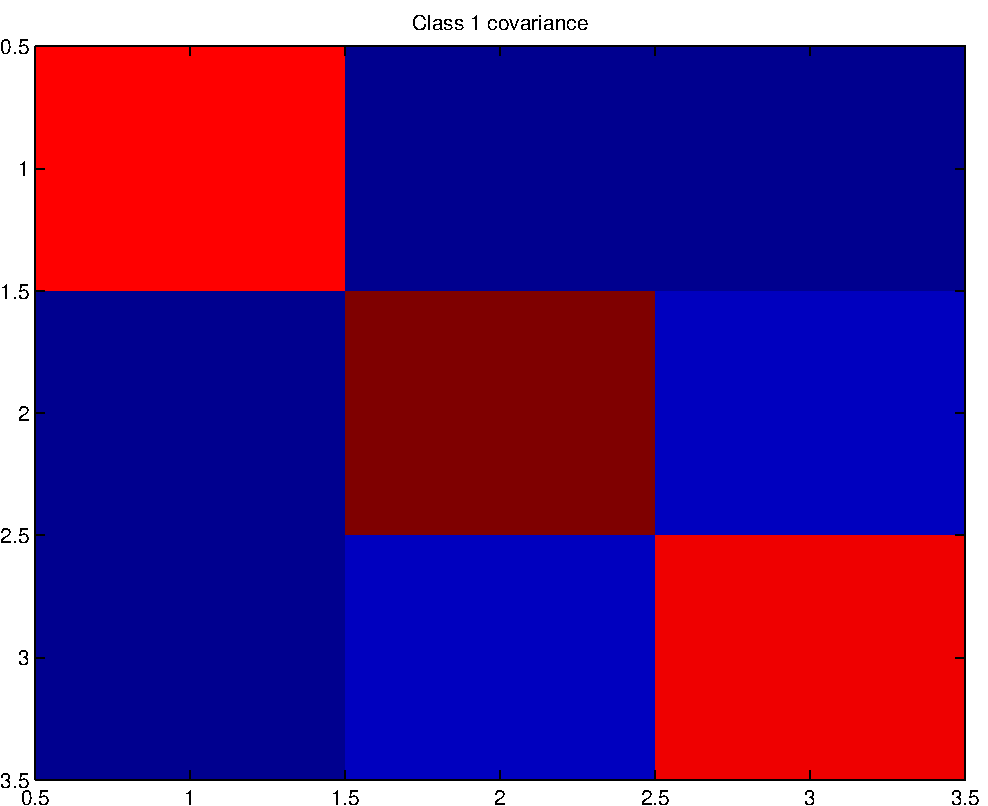
\includegraphics[width=10.0cm,height=10.0cm]{rv1_corr.pdf}

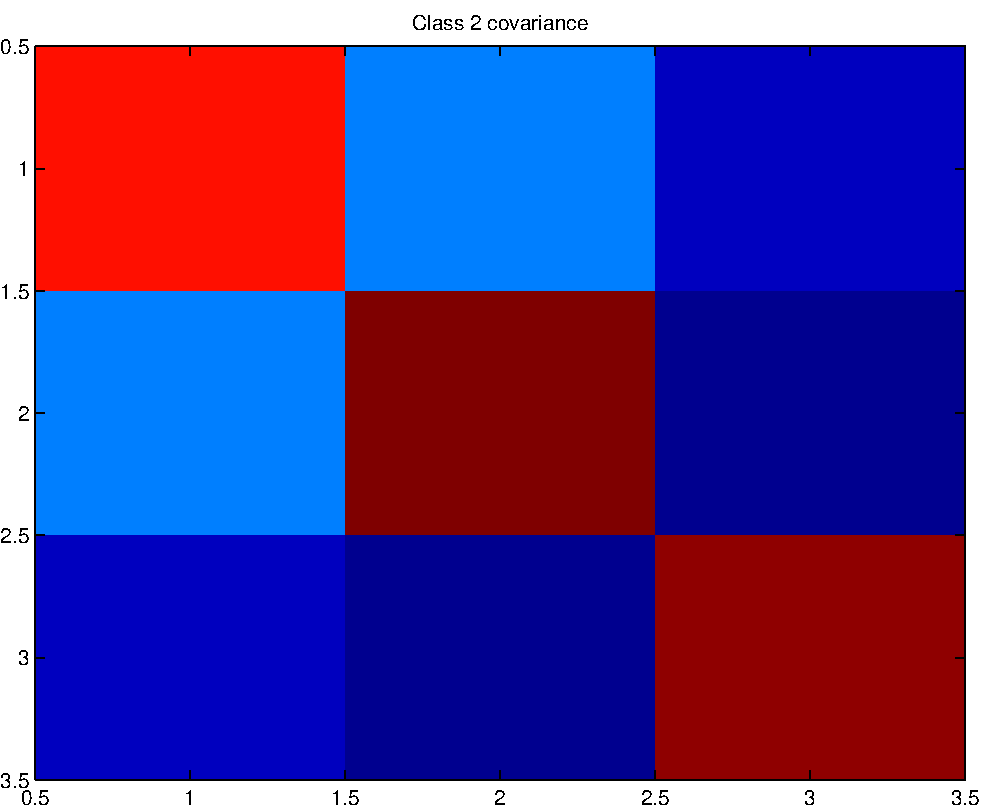
\includegraphics[width=10.0cm,height=10.0cm]{rv2_corr.pdf}

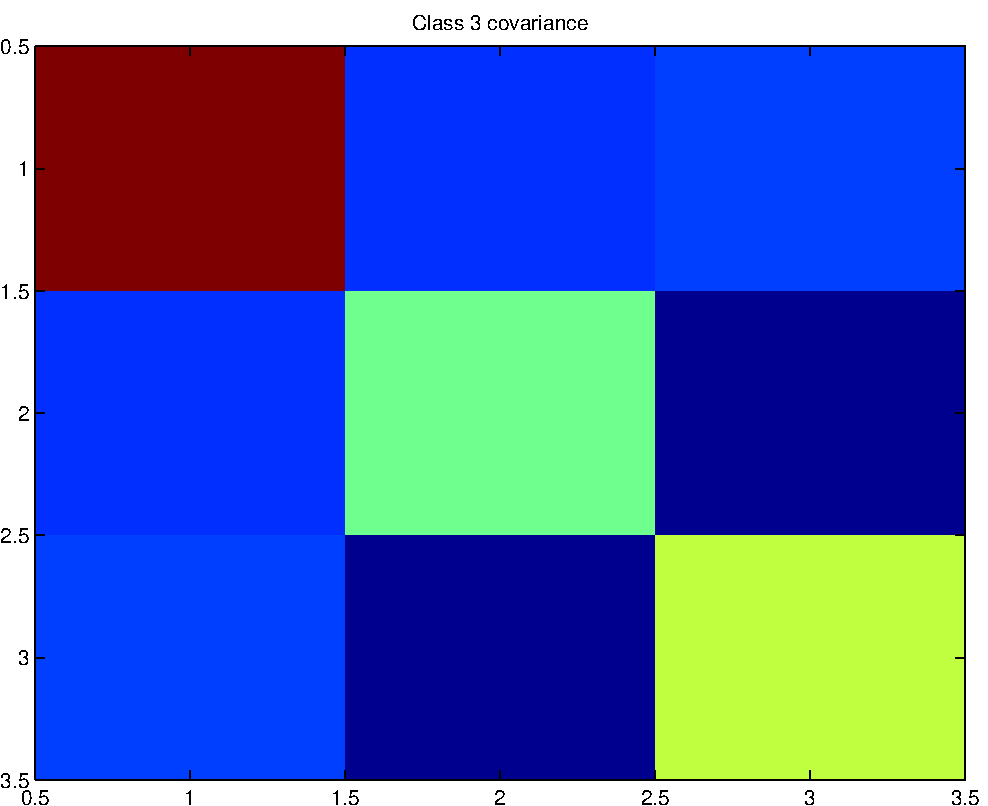
\includegraphics[width=10.0cm,height=10.0cm]{rv3_corr.pdf}

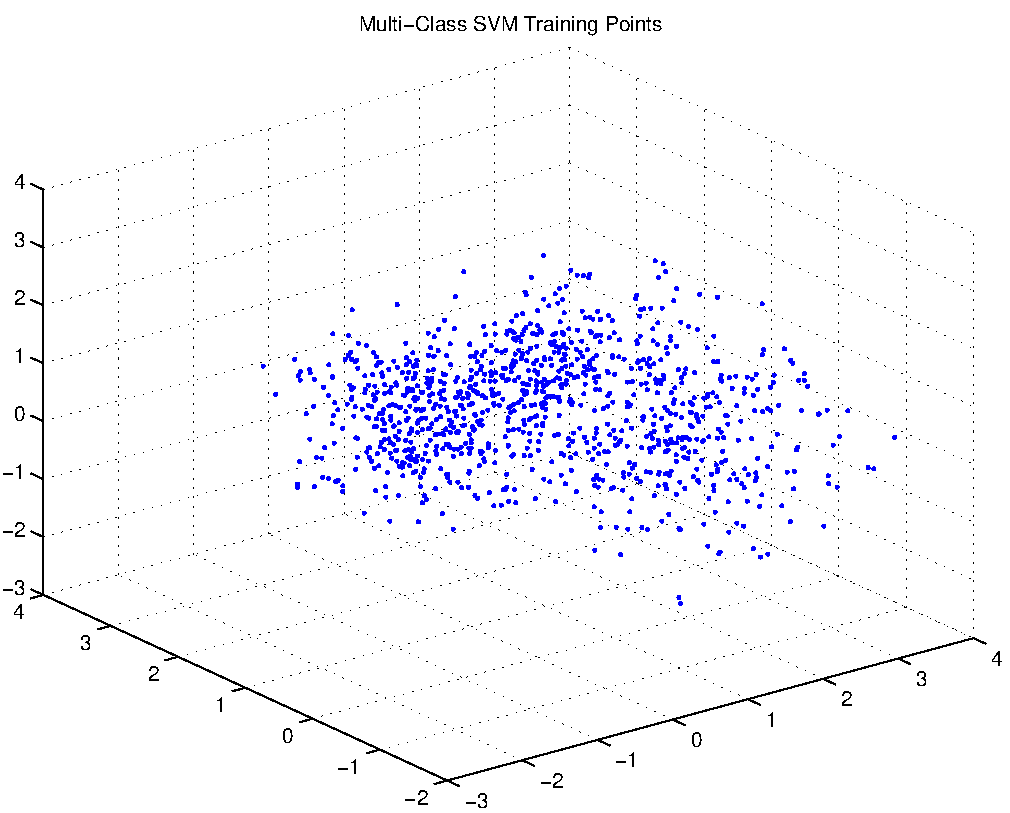
\includegraphics[width=10.0cm,height=10.0cm]{trainingPoints.pdf}

These are the SVM parameters - the RBF kernel is used\begin{itemize}
\item allOutlierFraction=0.05
\item mixingCoeff=0.3
\item smoThresh=1.0/10000.0
\item sigma=1
\end{itemize}
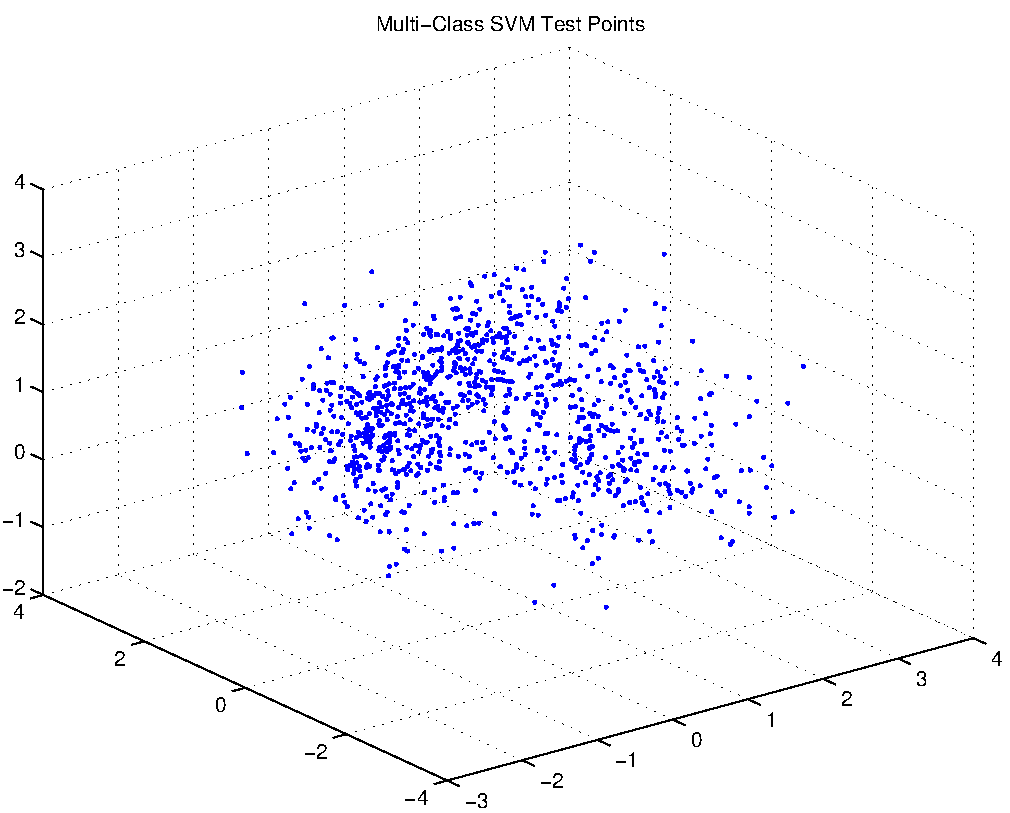
\includegraphics[width=10.0cm,height=10.0cm]{testPoints.pdf}

The marginal sample moments (mean var skew kurtosis) for training points.\newline
\begin{tabular}{ c |  c  c  c  c}
Feature & $\mu_1$ & $\mu_2$ & $\mu_3$ & $\mu_4$ \\
0 & +0.669 & +1.378 & +0.235& +2.430 \\
\hline
1 & +0.699 & +1.227 & +0.334& +2.332 \\
\hline
2 & +0.695 & +1.222 & +0.230& +2.329 \\
\hline
\end{tabular}
\newline
The marginal sample moments (mean var skew kurtosis) for test points.\newline
\begin{tabular}{ c | c  c  c  c}
Feature & $\mu_1$ & $\mu_2$ & $\mu_3$ & $\mu_4$ \\
0 & +0.677 & +1.288 & +0.363& +2.572\\
\hline
1 & +0.665 & +1.224 & +0.363& +2.312\\
\hline
2 & +0.718 & +1.158 & +0.239& +2.236\\
\hline
\end{tabular}\newline
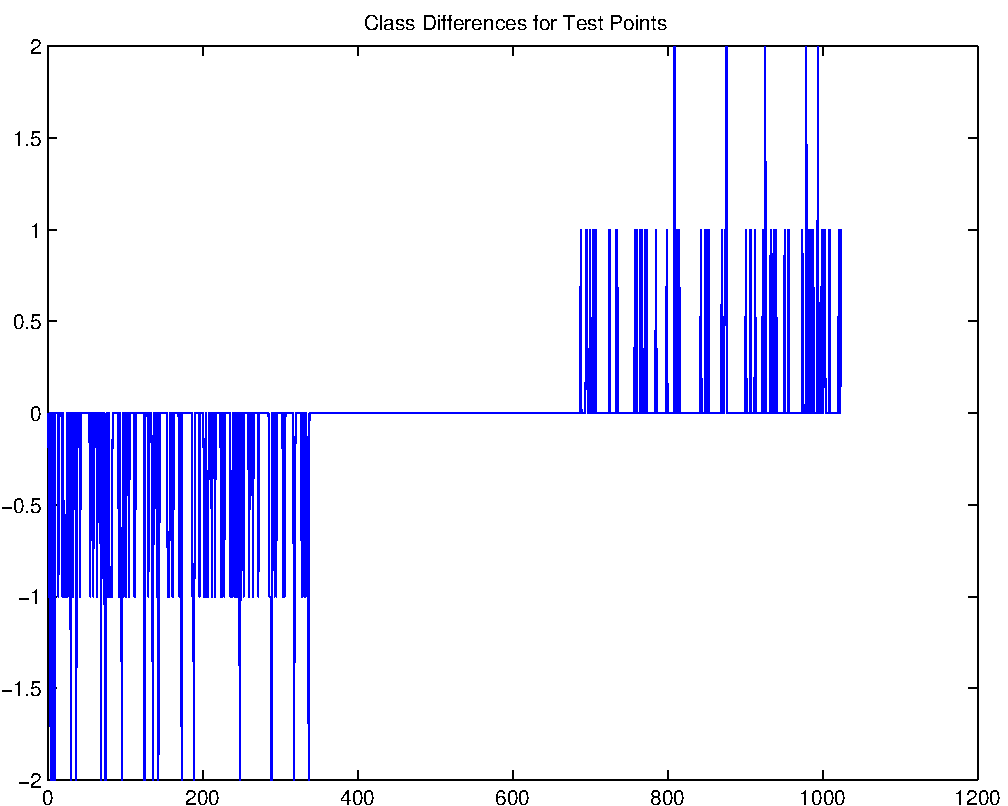
\includegraphics[width=10.0cm,height=10.0cm]{classDiffs.pdf}

The error rate for this run is +0.140\newline
QueryPerformanceCounter  =  +6.084
\subsubsection{Matrix Quick Check <double>}
QueryPerformanceCounter  =  +0.052
\subsubsection{Linear Regression atan data 3x1}
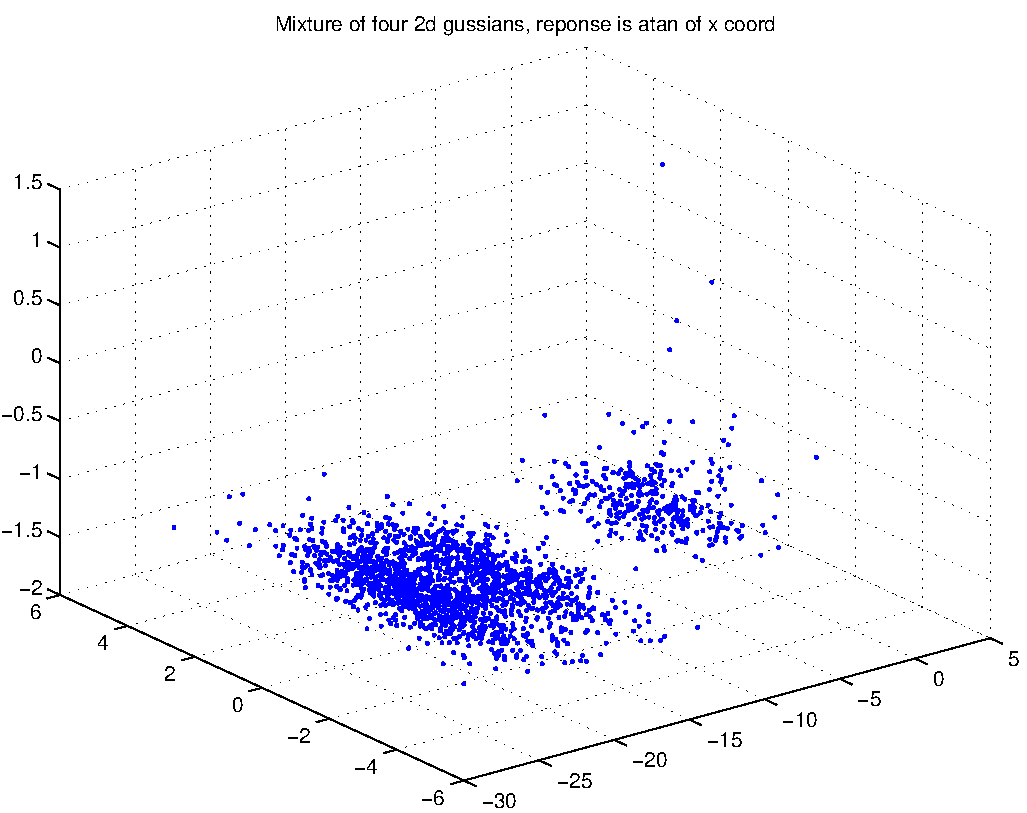
\includegraphics[width=10.0cm,height=10.0cm]{AtanDataSet.pdf}

\subsubsection{3 x 1 Linear Regression}
Sample size = 4000

Number of features = 3

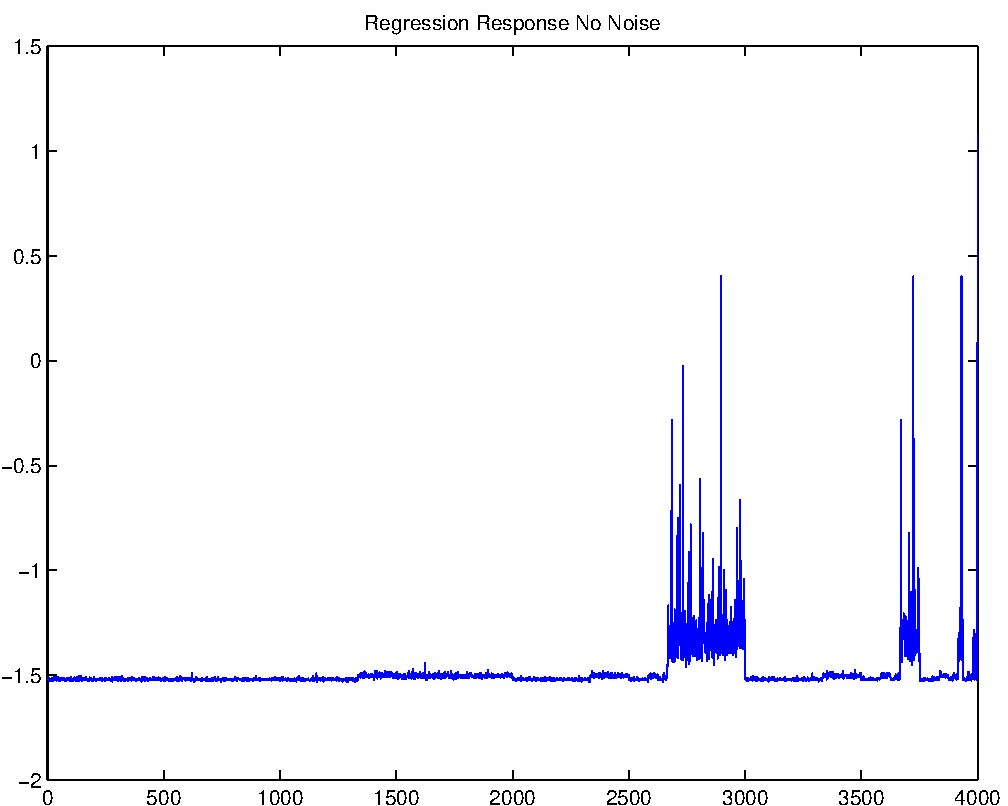
\includegraphics[width=10.0cm,height=10.0cm]{AtanDataSet_regression_response_no_noise.pdf}

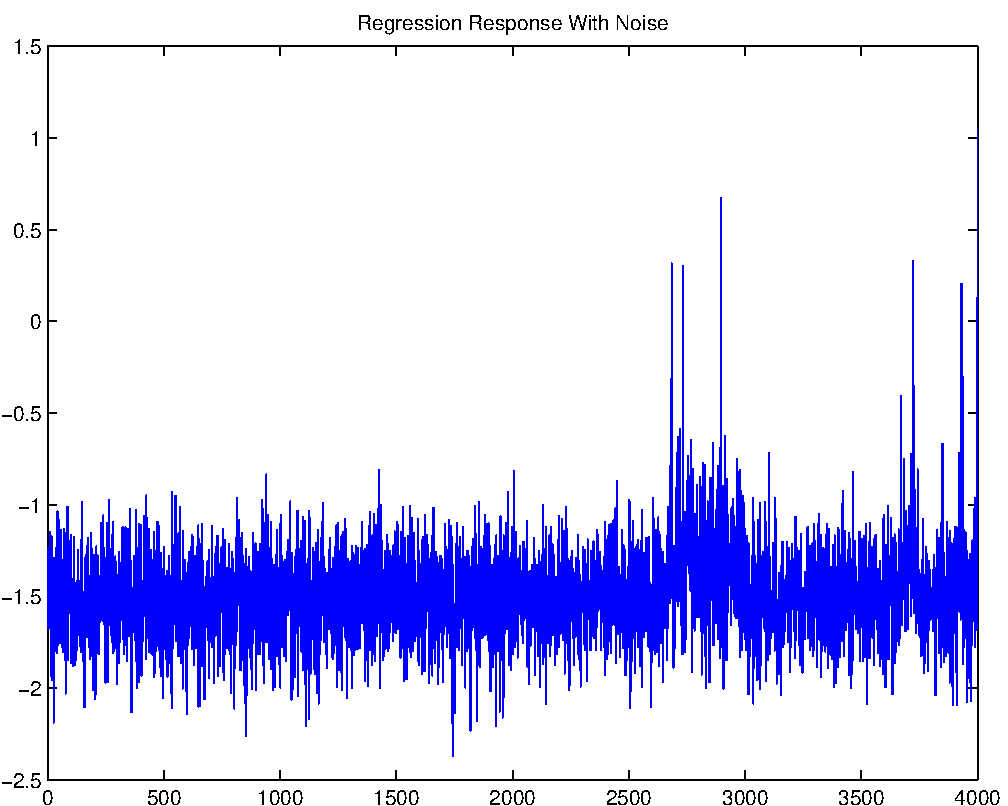
\includegraphics[width=10.0cm,height=10.0cm]{AtanDataSet_regression_response_with_noise.pdf}

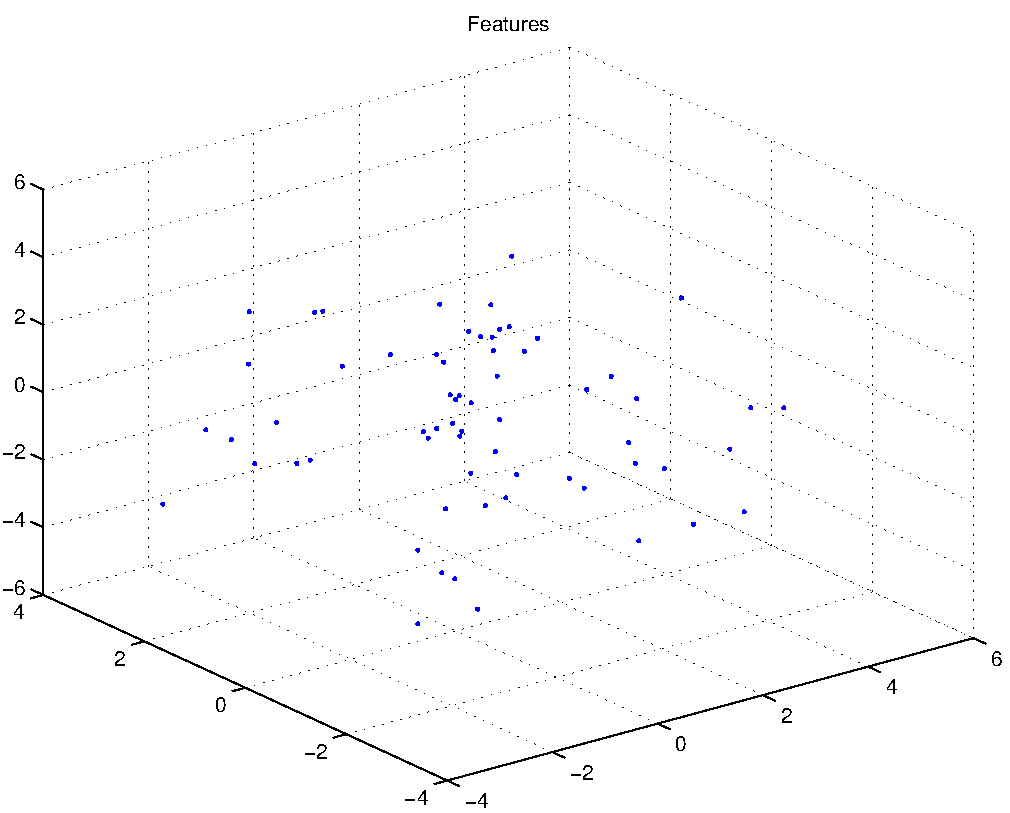
\includegraphics[width=10.0cm,height=10.0cm]{regression_features.pdf}

Response
-1.437
-1.671
-1.574
-1.238
-1.316
-1.340
-1.413
-1.285
-1.321
-1.147
-1.670
-1.381
-1.749
-1.504
-1.434
-1.934
-1.171
-1.374
-1.956
-1.602
-1.436
-1.536
-1.349
-1.869
-1.477
-2.187
-1.292
-1.390
-1.457
-1.760
-1.588
-1.355
-1.798
-1.788
-1.687
-1.235
-1.252
-1.509
-1.356
-1.813
-1.168
-1.381
-1.035
-1.260
-1.233
-1.766
-1.524
-1.702
-1.518
-1.084
-1.405
-1.286
-1.554
-1.754
-1.450
-1.665
-1.454
-1.137
-1.681
-1.685
-1.489
-1.777
-1.543
-1.650
-1.803
-1.299
-1.494
-1.710
-1.530
-1.499
-1.178
-1.130
-1.748
-1.235
-1.674
-1.846
-1.607
-2.029
-1.155
-1.598
-1.441
-1.534
-1.654
-1.034
-1.338
-1.012
-1.640
-1.498
-1.847
-1.557
-1.515
-1.394
-1.386
-1.529
-1.399
-1.592
-1.388
-1.235
-1.162
-1.863
-1.824
-1.528
-1.621
-1.840
-1.706
-1.835
-1.406
-1.494
-1.622
-1.628
-1.878
-1.445
-1.176
-1.378
-1.753
-1.612
-1.804
-1.424
-1.874
-1.546
-1.676
-1.632
-1.847
-1.734
-1.792
-1.559
-1.714
-1.465
-1.420
-1.246
-1.683
-1.607
-1.709
-1.669
-1.548
-1.506
-1.578
-1.770
-1.720
-1.416
-1.667
-1.457
-1.271
-1.767
-1.802
-1.191
-1.738
-0.987
-1.624
-1.778
-1.854
-1.533
-1.477
-1.733
-1.563
-1.645
-1.681
-1.483
-2.104
-1.709
-1.390
-1.303
-1.287
-1.418
-1.689
-1.598
-1.334
-1.225
-1.720
-1.501
-1.386
-1.485
-1.381
-1.194
-1.179
-1.535
-1.632
-1.777
-1.495
-1.386
-1.483
-1.591
-1.841
-1.593
-1.479
-1.825
-1.151
-1.220
-1.558
-1.452
-1.761
-1.239
-1.739
-1.394
-1.481
-1.421
-2.012
-1.410
-1.550
-1.614
-1.271
-1.365
-2.057
-1.751
-1.352
-1.404
-2.030
-1.407
-1.462
-1.226
-1.546
-1.282
-1.611
-1.739
-1.275
-1.393
-1.510
-1.809
-1.734
-1.522
-1.814
-1.435
-1.617
-1.502
-1.446
-1.391
-1.637
-1.533
-1.545
-1.097
-1.436
-1.384
-1.393
-1.181
-1.615
-1.631
-1.516
-1.440
-1.409
-1.057
-1.482
-1.532
-1.649
-1.632
-1.322
-1.742
-1.290
-1.451
-1.970
-1.517
-1.510
-1.432
-1.429
-1.366
-1.100
-1.549
-1.331
-1.579
-1.339
-1.954
-1.966
-1.476
-0.975
-1.321
-1.656
-1.192
-1.387
-1.239
-1.563
-1.633
-1.497
-1.269
-1.631
-1.436
-1.710
-1.443
-1.200
-1.752
-1.164
-1.809
-1.342
-1.464
-1.091
-1.797
-1.640
-1.599
-1.709
-1.565
-1.509
-1.356
-1.282
-1.779
-1.438
-1.311
-1.560
-1.510
-1.419
-1.483
-1.975
-1.971
-1.381
-1.447
-1.589
-1.548
-1.672
-1.607
-1.259
-1.863
-1.454
-1.749
-1.317
-1.425
-1.643
-1.320
-1.539
-1.572
-1.593
-1.509
-1.413
-1.124
-1.502
-1.503
-1.732
-1.407
-1.122
-1.593
-1.585
-1.814
-1.417
-1.607
-1.609
-1.423
-1.412
-1.567
-1.123
-1.653
-1.421
-1.210
-1.764
-1.282
-1.425
-1.179
-1.854
-1.318
-1.131
-1.631
-1.648
-1.700
-1.408
-1.434
-1.714
-1.366
-1.475
-1.253
-1.023
-1.088
-1.602
-1.491
-1.559
-1.499
-2.131
-1.452
-1.940
-1.525
-1.456
-1.679
-1.484
-1.625
-1.611
-1.682
-1.280
-1.493
-1.519
-1.695
-1.574
-1.466
-1.581
-1.728
-1.830
-1.027
-1.853
-1.380
-2.002
-1.798
-1.597
-1.622
-1.233
-1.715
-1.247
-1.362
-1.368
-1.965
-1.780
-1.106
-1.696
-1.288
-1.616
-1.874
-1.599
-1.374
-1.111
-1.620
-1.581
-1.933
-1.673
-1.548
-1.660
-1.531
-1.589
-1.490
-1.743
-1.413
-1.505
-1.450
-1.607
-1.287
-1.061
-1.341
-1.308
-1.523
-1.500
-1.840
-1.613
-1.239
-0.949
-1.586
-1.075
-1.726
-1.253
-1.442
-1.412
-1.199
-1.180
-1.381
-1.130
-1.561
-1.805
-1.690
-1.493
-1.389
-1.569
-1.597
-1.679
-1.314
-1.246
-1.398
-1.812
-1.300
-1.318
-1.455
-1.392
-1.320
-1.820
-1.640
-1.509
-1.939
-1.151
-1.235
-1.343
-1.619
-1.902
-1.557
-1.919
-1.783
-1.250
-1.751
-1.797
-1.528
-1.535
-1.200
-1.425
-1.663
-1.092
-1.173
-1.668
-1.773
-1.381
-1.116
-1.532
-1.793
-1.233
-1.721
-1.885
-1.334
-1.715
-1.516
-1.409
-1.262
-1.934
-1.466
-1.620
-1.531
-1.495
-1.524
-1.356
-1.440
-2.053
-1.347
-1.790
-1.602
-1.229
-1.284
-1.723
-1.487
-1.785
-1.590
-1.387
-1.519
-1.842
-1.418
-1.550
-1.515
-1.824
-1.623
-1.362
-1.936
-1.772
-1.531
-1.367
-1.411
-1.278
-1.803
-1.477
-1.764
-1.865
-1.763
-1.848
-1.459
-1.386
-1.499
-1.393
-2.026
-1.403
-1.494
-0.929
-1.562
-2.110
-1.337
-1.394
-1.220
-1.434
-1.311
-1.439
-1.651
-1.490
-1.447
-1.531
-1.420
-1.472
-0.953
-1.316
-1.723
-1.745
-1.542
-1.631
-1.486
-1.624
-1.394
-1.430
-1.451
-1.457
-1.156
-1.825
-1.540
-1.735
-1.466
-1.501
-1.612
-1.012
-1.537
-1.631
-1.501
-1.863
-1.660
-1.417
-1.837
-1.561
-1.576
-1.698
-1.638
-2.003
-1.344
-1.141
-1.693
-1.505
-1.541
-1.659
-1.395
-1.300
-1.472
-1.422
-1.785
-1.495
-1.593
-1.514
-1.373
-1.856
-2.142
-1.890
-1.533
-1.726
-1.518
-1.399
-1.732
-1.763
-1.316
-1.347
-1.613
-1.729
-1.256
-1.656
-1.661
-1.408
-1.429
-1.663
-1.305
-1.231
-1.498
-1.461
-1.785
-1.185
-1.251
-1.164
-1.183
-1.524
-1.347
-1.362
-1.536
-1.321
-1.875
-1.740
-1.650
-1.284
-1.692
-1.277
-1.295
-1.462
-1.780
-1.440
-1.356
-1.774
-1.273
-1.227
-1.305
-1.518
-1.764
-1.735
-1.112
-2.101
-1.275
-1.528
-1.635
-1.189
-2.096
-1.214
-1.542
-1.428
-1.565
-1.697
-1.594
-1.436
-1.708
-1.393
-1.881
-1.104
-1.289
-1.739
-1.307
-1.317
-1.626
-1.700
-1.670
-1.448
-1.761
-2.060
-1.580
-1.822
-1.841
-1.773
-1.393
-1.624
-1.664
-1.497
-1.311
-1.462
-1.418
-1.340
-1.308
-1.737
-1.484
-1.356
-1.314
-1.946
-1.246
-1.510
-1.674
-1.429
-1.732
-1.746
-1.734
-1.400
-1.565
-1.747
-1.622
-1.427
-1.400
-1.480
-1.118
-1.776
-1.404
-1.649
-1.584
-1.723
-1.395
-1.971
-1.840
-1.406
-1.676
-1.288
-1.713
-1.485
-1.312
-1.227
-1.474
-1.522
-1.418
-1.611
-1.709
-1.287
-1.550
-1.169
-1.936
-1.530
-1.416
-1.323
-1.526
-1.533
-1.607
-1.709
-1.880
-1.327
-1.744
-1.517
-1.435
-1.272
-1.586
-1.508
-1.234
-1.456
-1.404
-1.228
-1.554
-1.439
-1.911
-1.296
-1.130
-1.537
-1.845
-1.502
-1.955
-1.332
-1.635
-1.433
-1.812
-1.189
-1.640
-1.769
-1.461
-1.538
-1.662
-1.347
-1.689
-1.783
-1.525
-1.675
-1.686
-1.746
-1.433
-1.745
-1.214
-1.321
-1.796
-1.591
-1.349
-1.813
-1.510
-1.561
-1.541
-2.024
-1.476
-1.649
-1.758
-1.653
-1.708
-1.258
-1.746
-1.526
-1.293
-1.459
-1.844
-1.417
-1.809
-2.111
-1.873
-1.403
-1.648
-1.374
-1.875
-1.182
-1.195
-1.305
-1.763
-1.592
-1.579
-0.965
-1.494
-1.339
-1.393
-1.547
-1.320
-1.083
-1.506
-1.524
-1.382
-1.472
-1.328
-1.797
-1.514
-1.560
-1.902
-1.519
-1.458
-1.178
-1.468
-1.470
-1.498
-1.153
-1.313
-1.490
-1.848
-1.447
-1.280
-1.634
-1.637
-1.981
-1.324
-1.497
-1.543
-2.081
-1.585
-1.818
-1.242
-1.624
-1.594
-2.261
-1.731
-1.804
-1.425
-1.340
-1.638
-1.532
-1.750
-1.780
-1.602
-1.482
-1.310
-1.703
-1.284
-1.654
-1.830
-1.537
-1.464
-1.681
-1.363
-1.675
-1.896
-1.690
-1.511
-1.811
-1.550
-2.006
-1.153
-1.508
-1.751
-1.353
-1.410
-1.623
-1.679
-1.647
-1.320
-1.510
-1.280
-1.563
-1.211
-2.009
-1.412
-1.465
-1.215
-1.689
-1.292
-1.803
-1.640
-1.284
-1.281
-1.814
-1.799
-1.258
-1.609
-1.599
-1.374
-1.752
-1.483
-1.295
-1.216
-1.815
-1.477
-1.546
-1.490
-1.741
-1.721
-1.396
-0.972
-1.601
-1.236
-1.576
-1.443
-1.023
-1.697
-1.878
-1.716
-1.973
-1.787
-1.750
-1.604
-1.310
-1.475
-1.099
-1.403
-1.408
-1.721
-0.834
-1.747
-1.380
-1.418
-1.556
-1.556
-1.055
-1.604
-1.522
-1.463
-1.840
-1.517
-1.404
-1.238
-1.341
-1.286
-1.826
-1.683
-1.473
-1.557
-1.896
-1.092
-1.599
-1.295
-1.681
-1.323
-1.779
-1.326
-1.683
-1.393
-2.011
-1.811
-1.589
-1.733
-1.473
-1.994
-1.563
-1.651
-1.330
-1.490
-1.271
-1.446
-1.569
-1.526
-1.136
-1.269
-1.823
-1.586
-1.479
-1.450
-1.451
-1.567
-1.347
-1.392
-1.870
-1.349
-1.598
-1.205
-1.105
-1.578
-1.997
-1.661
-1.056
-1.741
-1.606
-1.604
-1.281
-1.399
-1.776
-1.345
-1.603
-1.547
-1.356
-1.473
-1.324
-1.314
-1.825
-1.464
-1.550
-1.316
-1.299
-1.685
-1.345
-1.453
-1.558
-1.555
-1.854
-1.259
-1.545
-1.470
-1.534
-1.471
-1.402
-1.601
-1.192
-1.587
-1.256
-1.461
-1.229
-1.282
-1.511
-1.481
-1.571
-0.981
-1.574
-1.531
-1.631
-1.427
-2.063
-1.595
-1.806
-1.261
-1.449
-2.007
-1.722
-1.653
-1.727
-1.427
-1.568
-1.560
-1.376
-1.412
-1.480
-1.609
-1.937
-1.328
-1.246
-1.574
-1.393
-1.286
-1.324
-1.188
-1.699
-1.394
-1.034
-2.044
-1.834
-1.530
-1.406
-1.499
-1.479
-1.659
-1.243
-1.484
-1.615
-1.647
-1.593
-1.366
-1.380
-1.462
-1.199
-1.801
-1.489
-1.450
-1.602
-1.354
-1.286
-1.358
-1.771
-1.064
-1.902
-1.347
-1.335
-1.806
-1.087
-1.791
-1.367
-1.978
-1.537
-1.320
-2.204
-1.751
-1.539
-1.503
-1.786
-1.344
-1.331
-1.898
-1.578
-1.852
-1.548
-1.295
-1.692
-2.166
-1.035
-1.583
-1.071
-1.525
-1.794
-1.602
-1.922
-1.619
-1.495
-1.887
-1.485
-1.643
-1.414
-1.559
-1.574
-1.732
-1.372
-1.237
-1.323
-1.486
-1.667
-1.258
-1.506
-1.895
-1.393
-1.499
-1.921
-1.524
-1.349
-1.805
-1.206
-1.605
-1.650
-1.324
-1.249
-2.027
-1.765
-1.136
-1.736
-1.947
-1.747
-2.085
-1.861
-1.320
-1.595
-1.560
-1.314
-1.816
-1.475
-1.369
-1.736
-1.498
-1.179
-1.589
-1.241
-1.381
-1.600
-1.228
-0.990
-1.539
-1.342
-1.425
-1.585
-1.747
-1.532
-1.286
-1.349
-1.435
-1.628
-1.609
-1.558
-1.381
-1.739
-1.724
-1.719
-1.892
-1.370
-1.483
-1.699
-1.461
-1.451
-1.525
-1.481
-1.550
-1.518
-1.482
-1.678
-1.329
-1.182
-1.352
-1.368
-1.375
-1.616
-1.347
-1.473
-1.699
-1.665
-1.828
-1.488
-1.588
-1.768
-1.722
-1.295
-1.846
-1.289
-1.387
-1.807
-1.512
-1.458
-1.460
-1.674
-1.228
-1.526
-1.359
-1.319
-1.762
-1.179
-1.293
-1.111
-1.368
-1.995
-1.404
-1.493
-1.097
-1.540
-1.485
-1.776
-1.903
-1.635
-1.612
-1.691
-1.349
-1.254
-1.673
-1.253
-1.889
-1.675
-1.174
-1.674
-1.900
-2.009
-1.508
-1.167
-1.220
-1.465
-1.462
-1.149
-1.613
-1.662
-1.642
-1.371
-1.597
-1.599
-1.651
-1.495
-1.719
-1.077
-1.735
-1.438
-1.134
-1.322
-1.721
-1.662
-2.055
-1.487
-1.366
-1.753
-1.294
-1.393
-1.559
-1.777
-1.602
-1.558
-1.710
-1.369
-1.724
-1.534
-1.309
-1.643
-1.524
-1.616
-1.638
-1.794
-1.224
-2.001
-1.602
-1.252
-1.368
-1.516
-1.265
-1.499
-1.290
-1.460
-1.817
-1.395
-1.708
-1.726
-1.301
-1.275
-1.790
-1.750
-1.225
-1.526
-1.706
-1.666
-1.684
-1.526
-1.453
-1.787
-1.236
-1.782
-1.785
-1.562
-1.482
-1.388
-1.372
-1.659
-1.534
-1.663
-1.783
-1.419
-1.324
-1.414
-1.578
-1.256
-1.233
-1.477
-1.095
-1.644
-1.373
-1.617
-1.347
-1.369
-1.300
-1.321
-1.249
-1.524
-1.686
-1.335
-1.852
-1.958
-1.242
-1.845
-1.684
-1.522
-1.595
-1.849
-1.445
-1.532
-1.220
-1.335
-1.354
-1.987
-1.689
-1.408
-1.514
-1.627
-1.113
-1.504
-1.301
-1.543
-1.340
-1.794
-1.039
-1.174
-1.175
-1.637
-1.562
-1.555
-1.313
-1.872
-1.336
-1.332
-1.626
-1.166
-1.815
-1.199
-1.426
-1.582
-1.604
-1.051
-1.805
-1.854
-1.215
-1.671
-1.387
-1.111
-1.488
-1.365
-1.116
-1.558
-1.401
-1.715
-1.172
-1.543
-1.557
-1.354
-1.463
-1.306
-0.808
-1.301
-1.554
-1.647
-1.529
-1.706
-1.231
-2.001
-1.506
-1.001
-1.364
-1.415
-1.385
-1.696
-1.531
-1.195
-1.588
-1.371
-1.845
-1.379
-1.357
-1.439
-1.486
-1.822
-1.358
-1.749
-1.718
-1.468
-1.784
-1.251
-1.595
-1.489
-1.435
-1.627
-1.783
-1.492
-1.162
-1.714
-1.518
-1.213
-1.800
-1.474
-1.439
-1.659
-1.780
-1.321
-1.309
-1.631
-1.252
-1.626
-1.692
-1.564
-1.285
-1.425
-1.640
-1.280
-1.517
-1.289
-1.278
-1.516
-1.422
-1.745
-1.411
-1.346
-1.221
-1.518
-1.494
-1.297
-1.555
-1.144
-1.349
-1.643
-1.694
-1.278
-1.556
-1.574
-1.699
-1.417
-1.094
-1.489
-1.147
-1.234
-1.611
-1.113
-1.544
-1.679
-1.277
-1.410
-1.663
-1.627
-1.527
-1.365
-1.473
-1.541
-1.833
-1.538
-1.493
-1.147
-1.362
-1.156
-1.665
-1.644
-1.589
-1.404
-1.009
-1.420
-1.498
-1.786
-1.445
-1.962
-1.366
-1.336
-1.833
-1.547
-1.183
-1.638
-1.694
-1.323
-1.556
-1.424
-1.952
-1.365
-1.612
-1.502
-1.379
-1.775
-1.333
-1.169
-1.636
-1.172
-1.425
-1.172
-1.427
-1.801
-1.007
-1.757
-1.468
-1.579
-1.582
-1.832
-1.742
-1.109
-1.292
-1.326
-1.070
-1.411
-1.446
-1.799
-1.454
-1.556
-1.616
-1.604
-1.151
-1.338
-1.306
-1.519
-1.630
-1.745
-1.691
-1.517
-1.516
-1.671
-1.691
-1.651
-1.546
-1.427
-1.486
-1.715
-1.435
-1.850
-1.079
-1.370
-1.781
-1.614
-1.253
-1.873
-1.514
-1.714
-1.364
-1.632
-1.597
-1.322
-1.555
-1.688
-1.585
-1.271
-1.924
-1.190
-1.384
-1.574
-1.450
-1.719
-1.724
-1.176
-1.468
-1.482
-1.272
-1.908
-1.057
-1.457
-1.610
-1.626
-1.452
-1.672
-1.516
-1.578
-1.504
-1.164
-1.485
-1.496
-1.216
-1.579
-1.244
-1.352
-1.348
-1.294
-1.509
-1.971
-1.745
-1.546
-1.485
-1.448
-1.661
-1.834
-1.869
-1.529
-1.595
-1.378
-1.171
-1.608
-1.423
-1.931
-1.553
-1.782
-1.594
-1.726
-1.016
-1.380
-1.398
-1.779
-1.398
-1.671
-1.863
-1.326
-1.732
-1.739
-1.258
-1.687
-1.267
-1.288
-1.607
-1.436
-1.285
-1.494
-1.652
-1.471
-1.975
-1.614
-1.319
-1.500
-1.883
-1.737
-1.483
-1.524
-1.279
-1.590
-1.338
-1.295
-1.657
-1.693
-1.277
-1.318
-1.784
-1.697
-1.765
-1.688
-1.966
-1.434
-1.522
-1.564
-1.354
-1.707
-1.622
-1.629
-1.548
-1.104
-1.351
-1.520
-1.565
-1.483
-1.230
-1.663
-1.271
-1.583
-1.249
-1.773
-1.348
-1.259
-1.347
-1.324
-1.273
-1.701
-1.183
-1.477
-1.082
-1.558
-1.298
-1.225
-1.835
-1.692
-1.643
-1.114
-1.573
-1.442
-1.640
-1.543
-1.178
-1.952
-2.372
-1.326
-1.456
-1.781
-2.018
-1.661
-1.540
-1.542
-1.735
-1.657
-1.710
-2.134
-1.999
-1.300
-1.212
-1.565
-1.487
-1.416
-1.776
-1.395
-1.096
-1.630
-1.434
-1.721
-1.731
-1.642
-1.793
-1.355
-1.625
-1.485
-1.230
-1.178
-1.193
-1.353
-1.365
-1.655
-1.579
-1.297
-1.431
-1.852
-1.616
-1.874
-1.432
-1.215
-1.123
-1.443
-1.456
-1.522
-1.444
-1.616
-1.530
-1.379
-1.445
-1.378
-1.285
-1.997
-1.318
-1.746
-1.604
-1.670
-1.490
-1.569
-1.569
-1.800
-1.251
-1.533
-1.483
-1.371
-1.782
-1.277
-1.523
-1.450
-1.647
-1.780
-1.338
-1.640
-1.872
-2.231
-1.433
-1.561
-1.351
-1.642
-1.231
-1.347
-1.682
-1.570
-1.427
-1.660
-1.187
-1.431
-1.261
-1.665
-1.625
-1.532
-1.571
-1.712
-1.005
-1.687
-1.726
-1.270
-1.160
-1.479
-1.790
-1.671
-1.711
-1.576
-2.178
-1.332
-1.326
-1.832
-1.698
-1.486
-1.408
-1.561
-0.986
-1.872
-1.528
-1.252
-1.440
-1.883
-1.722
-1.308
-1.232
-1.554
-1.421
-1.494
-1.672
-1.275
-1.433
-1.724
-1.548
-1.356
-1.239
-1.296
-1.256
-1.509
-1.460
-1.319
-1.055
-1.587
-1.452
-1.709
-1.201
-1.533
-1.350
-1.705
-1.564
-1.487
-1.105
-1.342
-1.665
-1.441
-1.739
-1.321
-1.432
-1.102
-1.799
-1.513
-1.223
-1.222
-1.738
-1.781
-1.816
-2.016
-1.584
-1.505
-1.415
-1.624
-1.329
-1.474
-1.879
-1.375
-1.645
-1.887
-1.408
-1.622
-1.659
-1.603
-1.295
-1.347
-1.681
-1.347
-1.220
-1.388
-1.700
-1.896
-1.560
-2.207
-1.167
-1.610
-1.494
-1.710
-1.397
-1.558
-1.638
-1.365
-1.277
-1.799
-1.467
-1.693
-1.624
-1.671
-1.503
-2.127
-1.470
-1.345
-1.063
-1.328
-1.268
-1.286
-1.158
-1.389
-1.620
-1.382
-1.429
-2.161
-1.829
-1.635
-1.252
-1.271
-1.167
-2.047
-1.618
-1.236
-1.700
-1.684
-1.655
-1.260
-1.301
-1.101
-1.384
-1.493
-1.319
-1.370
-1.515
-1.676
-1.371
-1.538
-1.449
-0.929
-1.586
-1.288
-1.761
-1.414
-1.733
-1.873
-1.761
-1.481
-1.409
-1.342
-1.900
-1.303
-1.313
-1.449
-1.119
-1.450
-1.455
-1.170
-1.692
-1.281
-1.816
-1.761
-1.570
-0.816
-1.509
-0.906
-1.535
-1.774
-1.378
-1.541
-1.674
-1.148
-1.344
-1.407
-1.413
-1.740
-1.335
-1.295
-1.691
-1.661
-1.833
-1.438
-1.628
-1.545
-1.492
-1.539
-1.461
-1.288
-1.594
-1.456
-1.224
-1.584
-1.438
-1.362
-1.510
-1.561
-1.652
-1.365
-1.393
-1.455
-1.714
-1.638
-1.690
-1.756
-1.299
-1.201
-1.515
-1.438
-1.456
-1.628
-1.429
-1.311
-1.605
-1.436
-1.547
-1.445
-1.609
-1.618
-1.239
-1.701
-1.089
-1.411
-1.882
-1.431
-1.741
-1.741
-1.806
-1.506
-1.367
-1.547
-1.979
-1.418
-1.770
-1.699
-1.360
-1.537
-1.371
-1.763
-1.542
-1.552
-1.355
-1.326
-1.565
-1.511
-1.573
-1.665
-1.384
-1.406
-1.438
-1.382
-1.182
-1.300
-1.268
-1.330
-1.928
-1.783
-1.800
-1.366
-1.479
-1.374
-1.594
-1.327
-1.496
-1.363
-1.687
-1.566
-1.547
-1.500
-1.825
-1.810
-1.249
-1.632
-1.684
-1.510
-1.805
-1.995
-1.309
-1.653
-1.317
-1.576
-1.433
-1.751
-1.515
-1.273
-1.640
-1.306
-1.358
-1.303
-1.871
-1.001
-1.475
-1.333
-1.462
-1.355
-1.243
-1.469
-1.495
-1.358
-1.828
-1.653
-1.537
-1.119
-2.087
-1.695
-1.417
-1.538
-1.640
-1.681
-1.414
-1.753
-1.642
-1.438
-1.468
-1.322
-1.486
-1.402
-1.491
-1.167
-1.452
-1.529
-1.823
-1.471
-1.179
-1.763
-1.119
-1.283
-1.714
-1.671
-1.373
-1.229
-1.305
-1.216
-1.665
-1.710
-1.274
-1.508
-1.435
-1.590
-1.433
-1.874
-1.580
-1.428
-1.705
-1.394
-1.563
-1.616
-1.763
-1.467
-1.491
-1.688
-1.695
-1.815
-1.666
-1.406
-1.563
-1.189
-1.777
-1.283
-1.060
-1.749
-1.458
-1.704
-1.403
-1.414
-1.398
-1.438
-1.651
-1.562
-1.545
-1.148
-1.517
-1.223
-1.076
-1.700
-1.569
-1.504
-1.743
-1.647
-1.473
-1.363
-1.681
-1.140
-1.921
-1.724
-1.609
-1.444
-1.456
-1.421
-1.012
-1.614
-1.297
-1.650
-1.461
-1.130
-1.756
-1.673
-1.789
-1.298
-1.629
-2.009
-1.667
-1.381
-1.347
-1.334
-1.984
-1.382
-1.336
-1.302
-1.313
-1.285
-1.505
-1.524
-1.467
-1.250
-1.305
-1.633
-1.365
-1.352
-1.685
-1.627
-1.726
-1.693
-1.873
-1.479
-1.742
-1.700
-1.370
-1.540
-1.526
-1.291
-1.552
-1.653
-1.716
-1.579
-1.350
-1.496
-1.405
-1.503
-1.163
-1.728
-1.769
-1.783
-1.843
-1.640
-1.308
-1.593
-1.594
-1.903
-1.385
-1.711
-1.814
-1.992
-1.422
-1.522
-1.520
-1.554
-1.493
-1.585
-1.510
-1.441
-1.535
-1.330
-1.230
-1.244
-1.257
-1.760
-1.246
-1.480
-1.393
-1.793
-1.247
-1.328
-1.760
-1.539
-1.585
-1.516
-1.325
-1.371
-1.437
-1.484
-1.963
-1.188
-1.531
-1.523
-1.389
-1.583
-1.511
-1.436
-1.451
-1.597
-1.620
-1.415
-1.417
-1.793
-1.780
-1.488
-1.253
-1.426
-1.712
-1.444
-1.690
-1.388
-1.406
-1.577
-1.713
-1.513
-1.199
-1.306
-1.724
-1.449
-1.330
-1.675
-1.533
-1.380
-1.309
-1.539
-1.381
-1.790
-1.649
-1.671
-1.148
-1.371
-1.138
-1.377
-1.578
-1.163
-1.272
-1.503
-1.285
-1.569
-1.356
-1.473
-1.510
-1.257
-1.548
-1.415
-1.373
-1.792
-1.393
-1.335
-1.481
-1.543
-1.404
-1.360
-1.502
-1.566
-1.641
-1.542
-1.418
-1.569
-1.550
-1.776
-1.505
-1.537
-1.093
-1.275
-1.542
-1.928
-1.667
-1.408
-1.546
-1.494
-1.334
-1.575
-1.453
-1.194
-1.841
-1.287
-1.631
-1.815
-1.171
-1.325
-1.109
-1.370
-1.278
-1.340
-1.743
-1.371
-1.687
-1.436
-1.102
-1.614
-1.809
-1.467
-1.490
-1.276
-1.472
-1.439
-1.653
-1.242
-1.554
-1.478
-1.084
-1.476
-1.261
-1.396
-1.552
-1.367
-1.657
-1.474
-1.633
-1.018
-1.863
-1.555
-1.692
-1.347
-0.868
-1.276
-1.576
-1.635
-1.354
-1.704
-1.580
-1.700
-1.515
-1.453
-1.337
-1.661
-1.391
-1.514
-1.828
-1.581
-1.544
-1.696
-1.656
-1.383
-1.661
-1.273
-1.624
-1.137
-1.471
-1.423
-1.438
-1.782
-1.579
-1.564
-1.222
-1.516
-1.473
-1.579
-1.457
-1.671
-1.667
-1.245
-1.928
-1.546
-1.504
-1.529
-1.849
-1.634
-1.654
-1.652
-1.411
-1.606
-1.439
-1.701
-1.522
-1.200
-1.606
-0.974
-1.701
-1.750
-2.109
-1.567
-0.983
-1.479
-1.432
-1.718
-1.688
-2.016
-1.201
-1.691
-1.852
-1.734
-1.613
-1.087
-1.268
-1.125
-1.597
-1.728
-1.724
-1.238
-1.349
-1.629
-1.816
-1.918
-1.698
-1.472
-1.466
-1.232
-1.460
-1.441
-1.666
-1.688
-1.222
-1.289
-1.193
-1.549
-1.775
-1.320
-1.329
-1.466
-1.388
-1.544
-1.682
-1.404
-1.582
-1.244
-1.880
-1.199
-1.260
-1.553
-1.465
-1.982
-1.992
-1.029
-1.078
-1.599
-1.421
-1.610
-1.569
-1.369
-1.723
-1.263
-1.332
-1.396
-1.488
-1.676
-1.314
-1.611
-1.523
-1.307
-1.284
-1.688
-1.178
-1.389
-1.227
-1.484
-1.186
-1.470
-1.432
-1.651
-1.773
-1.648
-1.447
-1.434
-1.173
-1.466
-1.424
-1.658
-1.675
-1.801
-1.680
-2.102
-1.438
-1.642
-1.858
-1.501
-1.503
-1.663
-1.654
-1.415
-1.471
-0.961
-1.793
-1.778
-1.785
-1.079
-1.752
-1.237
-1.302
-1.814
-1.470
-1.497
-1.219
-1.275
-1.136
-1.582
-1.425
-1.804
-1.653
-1.328
-1.366
-1.454
-1.202
-1.069
-1.247
-1.880
-1.468
-1.484
-1.451
-1.250
-1.698
-1.717
-1.163
-1.496
-1.386
-1.752
-1.239
-1.441
-1.516
-1.265
-1.735
-1.256
-1.969
-1.404
-1.427
-1.381
-1.453
-1.631
-1.612
-1.569
-1.672
-1.353
-1.436
-1.451
-1.323
-1.565
-1.590
-1.398
-1.474
-1.848
-1.565
-1.171
-1.516
-1.394
-1.010
-1.670
-1.249
-1.445
-1.158
-1.476
-1.429
-1.320
-0.787
-1.058
-1.428
-1.537
-1.081
-0.630
-1.508
-1.171
+0.316
-1.328
-1.387
-0.916
-1.394
-1.415
-1.518
-1.478
-1.888
-1.320
-1.864
-1.222
-1.664
-1.300
-1.379
-1.779
-1.357
-1.452
-1.527
-1.188
-0.905
-1.495
-1.523
-0.897
-1.409
-0.834
-0.629
-1.385
-1.554
-1.464
-1.525
-1.215
-0.976
-0.955
-0.886
-1.322
-1.155
-0.586
-1.058
-1.276
-1.657
-1.313
-1.393
-1.096
-1.144
-1.302
-1.355
-1.814
-1.008
-1.589
+0.302
-1.419
-1.625
-1.354
-1.251
-1.093
-1.248
-1.229
-1.039
-1.801
-1.349
-1.356
-1.734
-1.396
-1.285
-1.094
-1.005
-1.141
-0.868
-1.330
-1.258
-0.735
-1.013
-0.919
-1.082
-0.845
-1.180
-1.375
-0.987
-1.108
-1.436
-1.466
-0.645
-1.459
-1.469
-1.109
-1.695
-1.913
-1.373
-1.476
-1.226
-0.807
-1.282
-1.488
-1.143
-1.611
-1.499
-1.440
-1.657
-1.687
-1.395
-1.234
-1.141
-1.048
-1.188
-1.473
-1.185
-1.336
-1.470
-1.611
-0.890
-1.435
-1.248
-1.573
-1.289
-1.336
-1.175
-1.287
-1.609
-1.307
-1.606
-0.847
-1.368
-1.480
-1.339
-0.900
-1.267
-1.466
-1.377
-1.926
-1.130
-1.014
-1.260
-1.598
-1.702
-0.998
-0.771
-1.244
-0.962
-1.530
-1.385
-1.492
-0.783
-1.166
-1.826
-1.301
-1.208
-1.158
-2.001
-1.672
-1.382
-1.591
-1.655
-1.403
-1.225
-0.981
-1.479
-1.114
-1.414
-1.468
-1.338
-1.450
-1.029
-1.967
-1.166
-0.854
-1.555
-1.577
-1.185
-1.521
-1.260
-0.977
-1.272
-1.499
-0.854
-1.210
-1.078
-1.350
-0.665
-0.754
-1.766
-1.181
-1.130
-1.673
-1.648
-1.502
-1.456
-1.607
-1.505
-1.521
-1.026
-1.342
-1.313
-1.646
-0.920
-1.272
-1.511
-0.926
-1.549
-1.730
-0.790
-1.246
-0.931
-0.961
-1.098
-1.099
-1.659
-1.601
-1.837
-0.693
-1.340
-1.446
+0.671
-1.427
-1.061
-1.596
-1.314
-1.778
-1.222
-0.895
-1.330
-1.274
-1.548
-2.002
-1.779
-1.845
-0.926
-1.263
-0.624
-1.444
-1.013
-1.376
-0.986
-1.370
-1.377
-0.969
-1.847
-1.593
-1.395
-0.858
-1.276
-1.054
-1.362
-1.582
-1.142
-1.439
-1.230
-1.287
-1.391
-1.371
-1.212
-1.279
-1.397
-1.313
-1.331
-1.022
-1.657
-1.122
-1.345
-1.324
-1.512
-1.010
-1.448
-1.010
-0.967
-0.977
-1.191
-1.058
-1.362
-1.592
-1.331
-1.262
-1.334
-1.240
-1.607
-1.188
-1.124
-1.247
-1.175
-1.619
-1.315
-0.749
-0.862
-1.098
-1.259
-1.209
-0.851
-0.820
-0.843
-1.203
-1.663
-1.557
-1.085
-1.833
-0.845
-1.266
-0.811
-1.068
-1.230
-1.366
-1.386
-1.482
-1.628
-1.102
-1.793
-1.487
-0.952
-1.424
-1.199
-1.392
-0.994
-1.691
-1.092
-0.989
-1.305
-1.234
-1.322
-1.458
-1.736
-1.592
-1.320
-1.790
-1.301
-1.169
-1.383
-1.648
-1.579
-1.206
-1.260
-1.413
-1.747
-2.032
-1.631
-1.618
-1.215
-1.544
-1.496
-1.506
-1.826
-1.741
-1.435
-1.593
-1.724
-1.559
-1.468
-1.474
-1.279
-1.520
-1.287
-1.929
-1.630
-0.962
-2.084
-1.571
-1.562
-1.096
-1.887
-1.600
-1.775
-1.338
-1.279
-1.592
-1.590
-1.823
-1.786
-1.516
-1.758
-1.322
-1.958
-1.562
-1.581
-1.081
-1.901
-1.948
-1.801
-1.671
-1.237
-1.810
-1.558
-1.198
-0.990
-2.006
-1.413
-1.874
-1.312
-1.508
-1.547
-1.280
-1.614
-1.594
-1.369
-1.547
-1.289
-1.276
-1.547
-1.255
-1.322
-1.359
-1.494
-1.672
-1.632
-1.656
-0.984
-1.458
-1.667
-1.962
-1.208
-1.096
-1.523
-1.571
-1.275
-1.438
-1.632
-1.501
-1.348
-1.228
-1.846
-1.804
-1.512
-0.715
-1.636
-1.789
-1.420
-1.564
-1.283
-1.816
-1.593
-1.583
-1.728
-1.525
-1.549
-1.524
-1.470
-1.635
-1.696
-1.551
-1.460
-1.210
-1.414
-1.619
-1.432
-1.573
-1.365
-1.795
-1.560
-1.397
-0.962
-1.492
-1.447
-1.244
-1.078
-1.639
-1.974
-1.519
-1.522
-1.562
-1.647
-1.733
-1.721
-1.521
-1.787
-1.448
-1.410
-1.371
-1.925
-1.529
-1.567
-1.687
-1.574
-1.520
-2.038
-1.333
-1.592
-1.645
-1.649
-1.576
-1.464
-1.201
-1.417
-1.774
-1.518
-1.586
-1.762
-1.761
-1.698
-1.585
-1.564
-1.408
-1.550
-1.686
-1.438
-1.399
-1.389
-1.526
-1.533
-1.587
-1.271
-1.398
-1.201
-1.537
-1.750
-1.238
-1.718
-1.236
-1.567
-1.605
-1.265
-1.716
-1.419
-1.910
-1.888
-1.685
-1.422
-1.773
-1.761
-1.421
-1.214
-1.253
-1.407
-1.347
-1.569
-1.318
-1.428
-1.294
-1.547
-1.507
-1.620
-1.448
-1.690
-1.637
-1.589
-1.836
-1.835
-1.065
-1.463
-1.660
-1.736
-1.246
-1.352
-1.419
-1.463
-1.238
-1.360
-1.442
-1.576
-1.409
-1.250
-1.764
-1.279
-1.564
-1.468
-1.355
-1.335
-1.872
-1.662
-1.160
-1.811
-1.646
-1.760
-1.582
-1.465
-1.788
-1.525
-1.915
-1.540
-1.565
-1.703
-1.453
-1.569
-1.705
-1.610
-1.499
-1.732
-1.662
-1.366
-1.416
-1.565
-1.512
-1.521
-1.404
-1.410
-1.574
-1.124
-1.577
-1.376
-1.465
-1.123
-1.548
-1.728
-1.405
-1.505
-1.641
-1.627
-1.408
-1.636
-1.227
-1.621
-1.791
-1.752
-1.763
-1.584
-1.773
-1.271
-1.635
-1.457
-1.210
-1.496
-1.315
-1.573
-1.823
-1.362
-1.452
-1.107
-1.792
-1.250
-1.198
-1.541
-1.336
-1.422
-1.494
-1.572
-1.434
-1.312
-1.614
-1.339
-1.513
-1.885
-1.538
-1.462
-1.104
-1.685
-1.563
-1.164
-1.048
-1.165
-1.661
-1.736
-1.629
-1.381
-1.576
-1.466
-1.166
-1.417
-1.531
-1.938
-1.782
-1.522
-1.318
-1.514
-1.519
-1.652
-1.311
-1.235
-1.234
-1.716
-1.764
-1.632
-1.514
-1.745
-1.242
-1.459
-1.800
-1.575
-1.164
-1.771
-1.467
-1.598
-1.104
-1.621
-1.690
-1.500
-1.677
-1.563
-1.889
-1.605
-1.500
-1.816
-1.586
-1.133
-1.492
-1.578
-1.450
-1.344
-1.738
-1.338
-1.420
-1.732
-1.818
-1.578
-1.494
-1.356
-1.489
-1.843
-1.533
-1.793
-1.217
-1.636
-1.646
-1.733
-1.278
-1.992
-1.167
-1.215
-1.549
-1.570
-1.701
-1.768
-1.541
-1.415
-1.971
-1.341
-1.734
-1.882
-1.659
-1.125
-1.795
-1.699
-1.886
-1.135
-1.372
-1.459
-1.634
-1.343
-1.463
-1.348
-1.831
-1.456
-1.676
-1.275
-1.547
-1.470
-1.508
-1.517
-1.294
-1.744
-0.997
-0.926
-1.011
-1.519
-1.159
-1.494
-1.824
-1.156
-1.332
-1.364
-1.307
-1.142
-1.453
-1.447
-1.682
-1.515
-1.366
-1.315
-1.616
-1.444
-1.533
-1.639
-1.426
-1.270
-1.594
-1.379
-1.243
-1.929
-1.155
-1.490
-1.257
-1.622
-1.242
-1.189
-1.523
-1.294
-1.357
-1.999
-1.351
-1.326
-1.640
-1.922
-1.575
-1.846
-1.314
-0.819
-1.526
-1.466
-1.328
-1.456
-1.286
-1.226
-1.583
-1.196
-1.418
-1.414
-1.592
-1.654
-1.679
-1.359
-1.340
-1.523
-1.644
-1.583
-1.564
-1.701
-1.697
-1.543
-1.441
-1.487
-1.596
-1.514
-1.402
-1.147
-1.285
-1.803
-1.270
-1.852
-1.371
-1.418
-1.419
-1.666
-1.321
-1.617
-1.506
-1.361
-1.185
-1.665
-1.321
-1.608
-1.853
-1.327
-1.409
-1.168
-1.673
-1.677
-1.768
-1.831
-1.448
-1.378
-1.484
-1.490
-1.104
-1.582
-1.465
-1.362
-1.345
-2.086
-1.516
-1.681
-1.449
-1.507
-1.605
-1.634
-1.633
-1.204
-1.508
-1.099
-1.835
-1.315
-1.467
-1.487
-1.317
-1.670
-1.447
-1.466
-1.371
-1.231
-1.429
-1.721
-1.724
-1.563
-1.595
-1.420
-1.434
-1.871
-1.189
-1.682
-1.495
-1.261
-1.494
-1.625
-1.168
-1.477
-1.427
-1.165
-1.433
-1.675
-1.489
-1.588
-1.472
-1.424
-1.809
-1.356
-1.643
-1.349
-1.683
-1.508
-1.622
-1.582
-1.880
-1.440
-1.308
-1.846
-1.567
-1.441
-1.595
-1.655
-1.843
-1.424
-1.843
-1.416
-1.545
-1.079
-1.771
-1.578
-1.925
-1.612
-1.258
-1.056
-1.681
-1.527
-1.586
-1.267
-1.345
-1.995
-1.793
-1.220
-1.554
-1.308
-1.387
-1.617
-1.648
-1.489
-1.649
-1.053
-1.007
-1.635
-1.841
-1.287
-1.396
-1.532
-1.434
-1.545
-1.440
-1.524
-1.404
-1.184
-1.352
-1.539
-1.072
-1.366
-1.503
-1.335
-1.641
-2.033
-1.182
-1.330
-1.674
-1.816
-1.458
-1.652
-1.642
-1.611
-1.846
-1.162
-1.860
-1.542
-1.803
-1.210
-1.352
-1.610
-1.363
-1.547
-1.743
-1.693
-1.380
-1.576
-1.733
-1.697
-1.581
-1.383
-1.134
-1.766
-1.749
-1.715
-1.318
-1.436
-1.727
-1.538
-1.188
-1.339
-0.406
-1.368
-1.537
-1.656
-1.298
-1.406
-1.460
-1.439
-1.512
-1.309
-1.217
-1.198
-1.299
-0.802
-0.749
-1.402
-1.266
-1.070
-1.139
-1.689
-1.127
-1.276
-1.267
-1.034
-1.277
-1.352
-1.439
-1.524
-1.304
-1.640
-1.413
-1.675
-1.121
-1.006
-1.347
-1.089
-1.323
-1.177
-1.107
-1.428
-1.145
-1.607
-0.928
-0.723
-1.413
-1.308
-1.506
-1.334
-1.405
-1.257
-1.192
-1.168
-1.432
+0.330
-1.221
-1.248
-0.990
-1.592
-1.191
-1.384
-0.917
-1.452
-1.358
-1.126
-1.361
-1.696
-1.465
-1.230
-1.285
-1.251
-1.358
-1.106
-0.807
-0.867
-1.107
-1.645
-1.497
-1.498
-1.357
-1.712
-1.638
-1.423
-1.446
-1.591
-1.824
-1.487
-1.376
-1.634
-1.381
-1.406
-1.432
-1.728
-1.299
-1.511
-1.820
-1.078
-1.336
-1.431
-1.682
-1.915
-1.841
-1.440
-1.862
-1.755
-1.386
-1.660
-1.414
-1.230
-1.750
-1.464
-1.267
-1.543
-1.359
-1.685
-1.506
-1.724
-1.420
-1.906
-1.427
-1.311
-1.309
-1.596
-1.685
-1.355
-1.534
-1.551
-1.445
-1.626
-1.479
-1.557
-1.582
-1.474
-1.624
-1.574
-1.587
-1.453
-1.636
-1.355
-1.688
-1.591
-1.451
-1.272
-1.622
-1.559
-1.406
-1.344
-1.649
-1.553
-2.040
-1.454
-1.810
-1.662
-1.750
-1.265
-1.415
-1.520
-1.137
-1.440
-1.618
-1.544
-1.425
-1.303
-1.179
-1.707
-1.810
-1.776
-1.558
-1.614
-1.514
-1.702
-1.099
-1.762
-1.370
-1.886
-1.772
-1.365
-1.530
-1.341
-0.669
-1.410
-1.615
-1.465
-1.449
-1.439
-1.264
-1.859
-1.387
-1.391
-1.519
-1.662
-1.552
-1.824
-1.770
-1.596
-1.711
-1.702
-1.500
-1.763
-1.093
-1.209
-1.177
-1.499
-1.427
-1.806
-1.577
-1.401
-1.324
-1.532
-1.342
-1.970
-1.141
-1.548
-1.685
-1.286
-1.371
-1.370
-1.434
-1.210
-1.986
-1.509
-1.701
-1.217
-2.092
-1.425
-1.733
-1.641
-1.344
-1.677
-1.585
-1.697
-1.184
-1.299
-1.228
-1.445
-1.120
-1.408
-1.910
-1.561
-1.390
-1.524
-1.541
-2.090
-1.643
-1.458
-1.296
-1.513
-1.131
-1.123
-1.438
-0.719
-1.578
-1.549
-1.037
-1.582
-1.494
-1.061
-1.626
-1.518
-1.480
-1.330
+0.205
-1.370
-1.622
-1.527
-1.118
-1.369
-0.301
-1.680
-1.871
-1.557
-1.651
-1.135
-1.774
-1.634
-1.308
-1.533
-1.393
-1.150
-1.539
-1.221
-1.641
-1.659
-1.779
-2.075
-1.387
-1.249
-1.361
-1.822
-1.945
-1.504
-1.912
-1.548
-1.332
-1.468
-1.298
-1.872
-1.268
-1.964
-1.638
-1.810
-2.069
-1.348
-1.528
-1.564
-1.765
-1.530
-1.705
-1.193
-1.521
-1.246
-1.614
-1.237
-1.479
-1.273
-1.590
-1.632
-1.027
-0.964
-1.649
-1.775
-1.469
-1.248
-1.425
-1.552
-1.441
-1.681
-1.080
-1.396
-1.142
+1.054
Estimate for Beta
-0.000
+0.002
+1.003
QueryPerformanceCounter  =  +5.762
\subsubsection{Linear Regression 3x1}
\subsubsection{3 x 1 Linear Regression}
Sample size = 64

Number of features = 3

$\sigma = \left(
\begin{array}{
ccc}
+3.952 & -0.499 & -0.010 \\
-0.499 & +1.895 & +0.465 \\
-0.010 & +0.465 & +4.477 \\
\end{array}
\right)$ \newline 

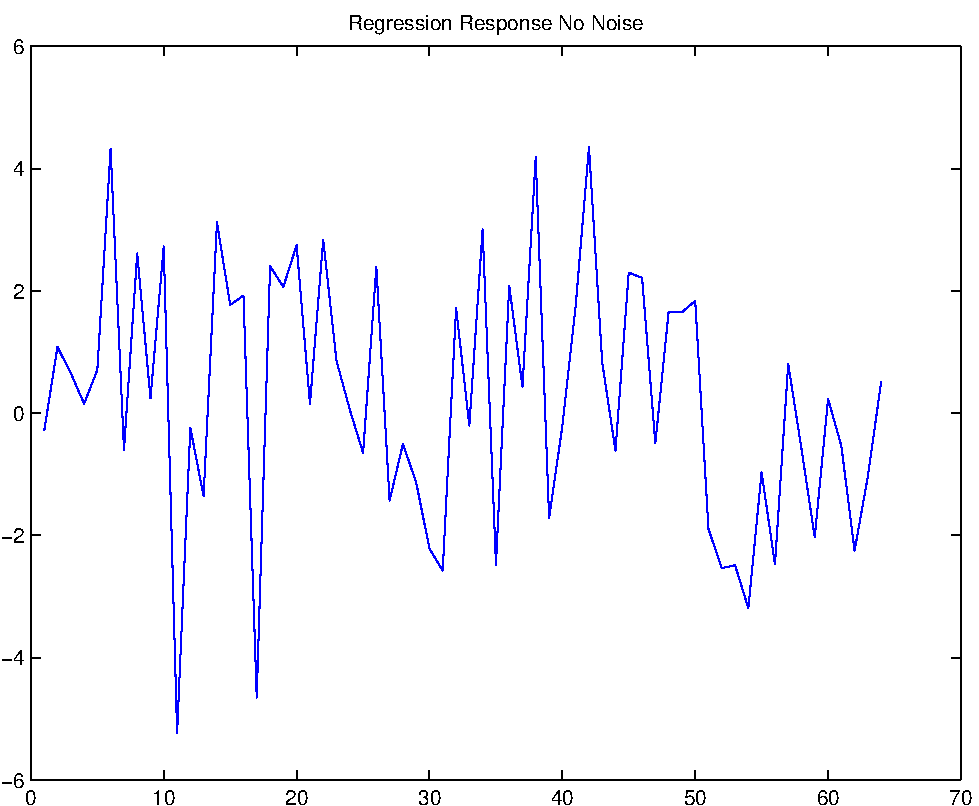
\includegraphics[width=10.0cm,height=10.0cm]{regression_response_no_noise.pdf}

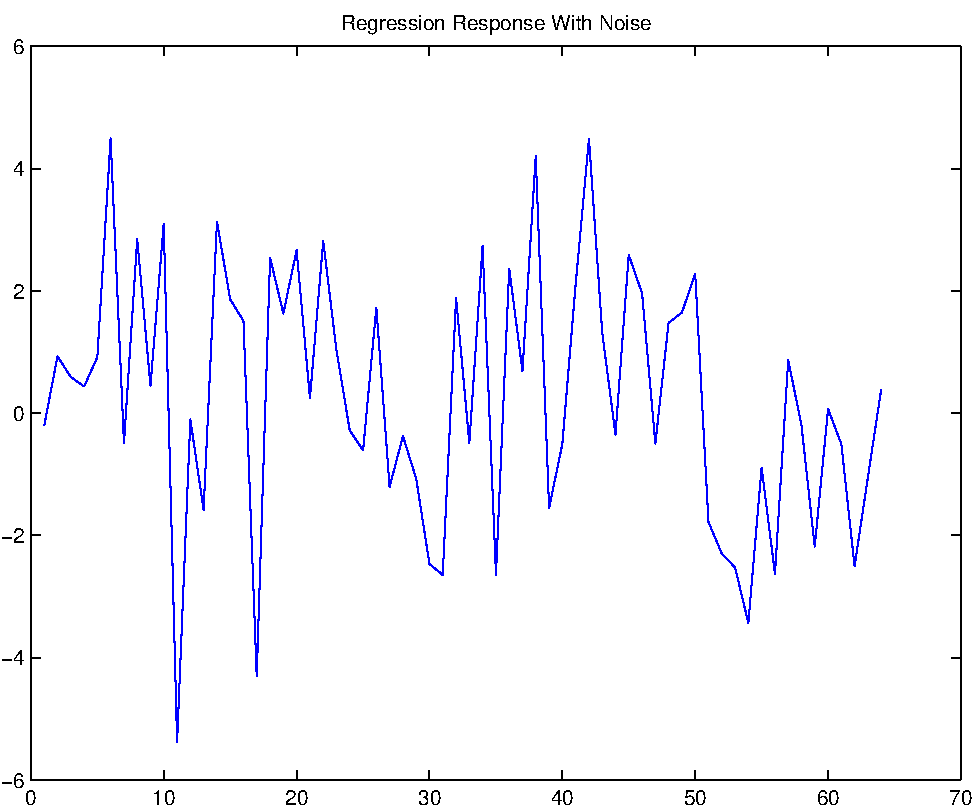
\includegraphics[width=10.0cm,height=10.0cm]{regression_response_with_noise.pdf}

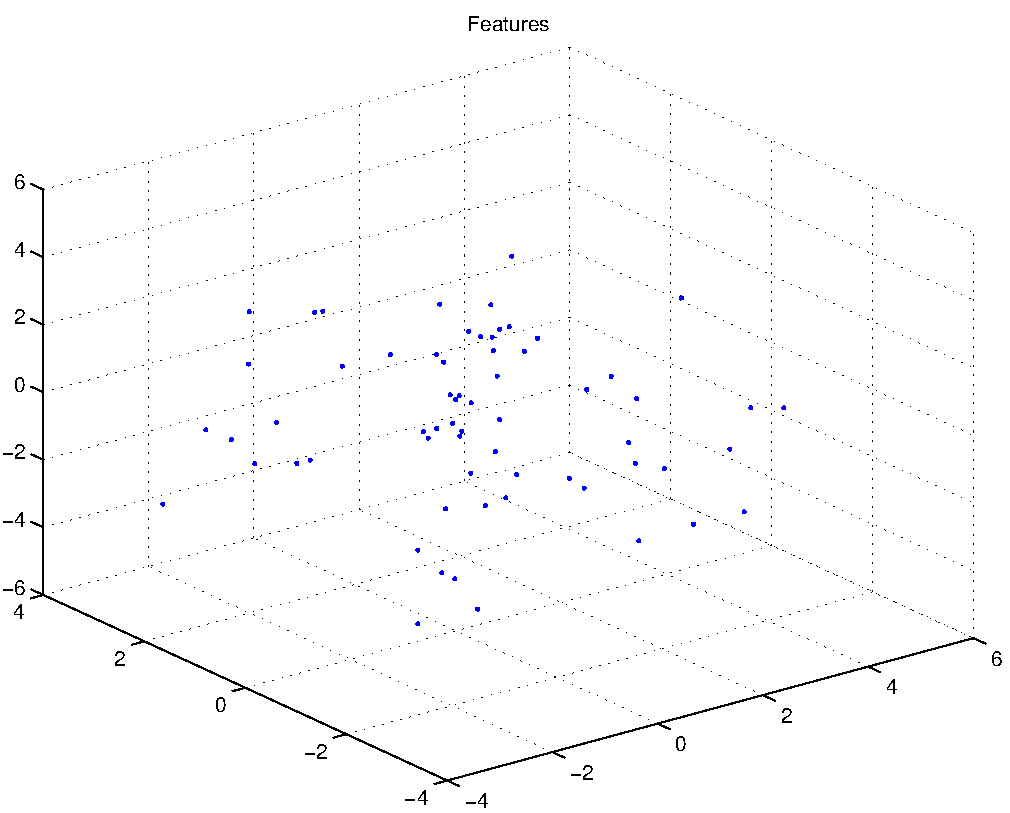
\includegraphics[width=10.0cm,height=10.0cm]{regression_features.pdf}

Beta
+0.817, +0.999, +0.510

Response
-0.208
+0.928
+0.595
+0.434
+0.915
+4.495
-0.493
+2.846
+0.449
+3.101
-5.387
-0.102
-1.584
+3.135
+1.860
+1.509
-4.307
+2.545
+1.628
+2.666
+0.244
+2.820
+1.026
-0.280
-0.610
+1.727
-1.207
-0.375
-1.074
-2.468
-2.648
+1.886
-0.489
+2.736
-2.642
+2.365
+0.688
+4.201
-1.552
-0.505
+2.093
+4.490
+1.318
-0.352
+2.589
+1.957
-0.498
+1.475
+1.647
+2.277
-1.779
-2.295
-2.527
-3.432
-0.892
-2.625
+0.869
-0.200
-2.185
+0.069
-0.507
-2.507
-1.057
+0.389
Estimate for Beta
+0.830
+1.010
+0.510
Error:
+0.013, +0.011, +0.000


QueryPerformanceCounter  =  +2.901
\subsubsection{Fast Gauss Transform}
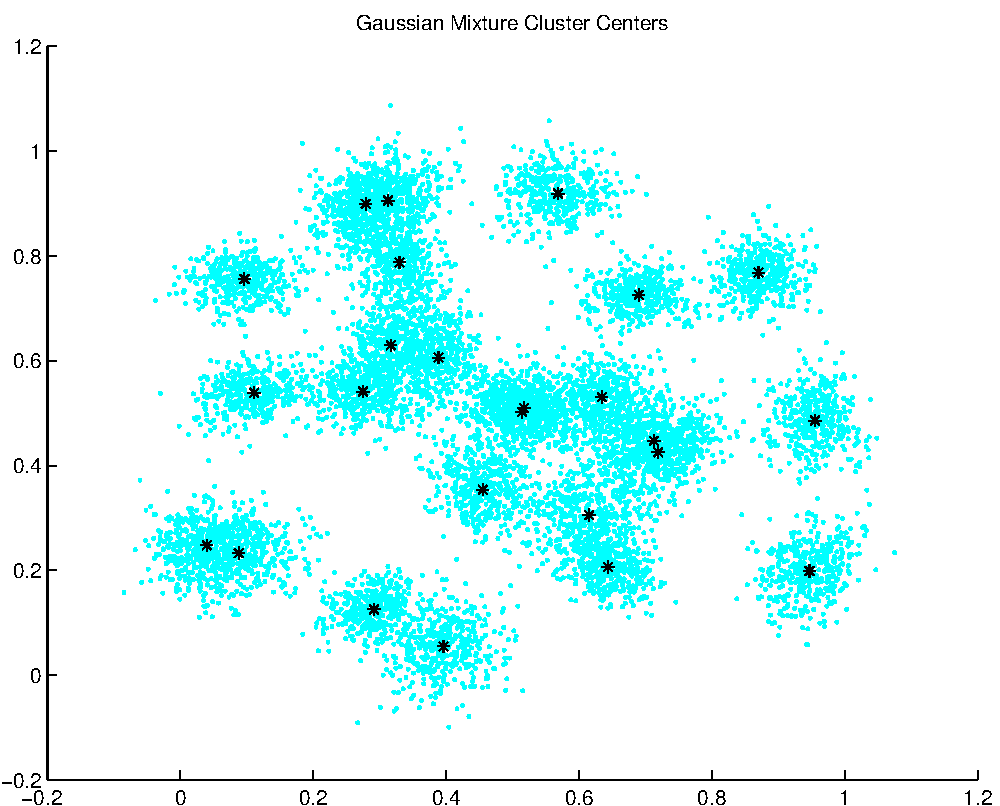
\includegraphics[width=10.0cm,height=10.0cm]{GaussianMixture_ClusterCenters25_Centers.pdf}

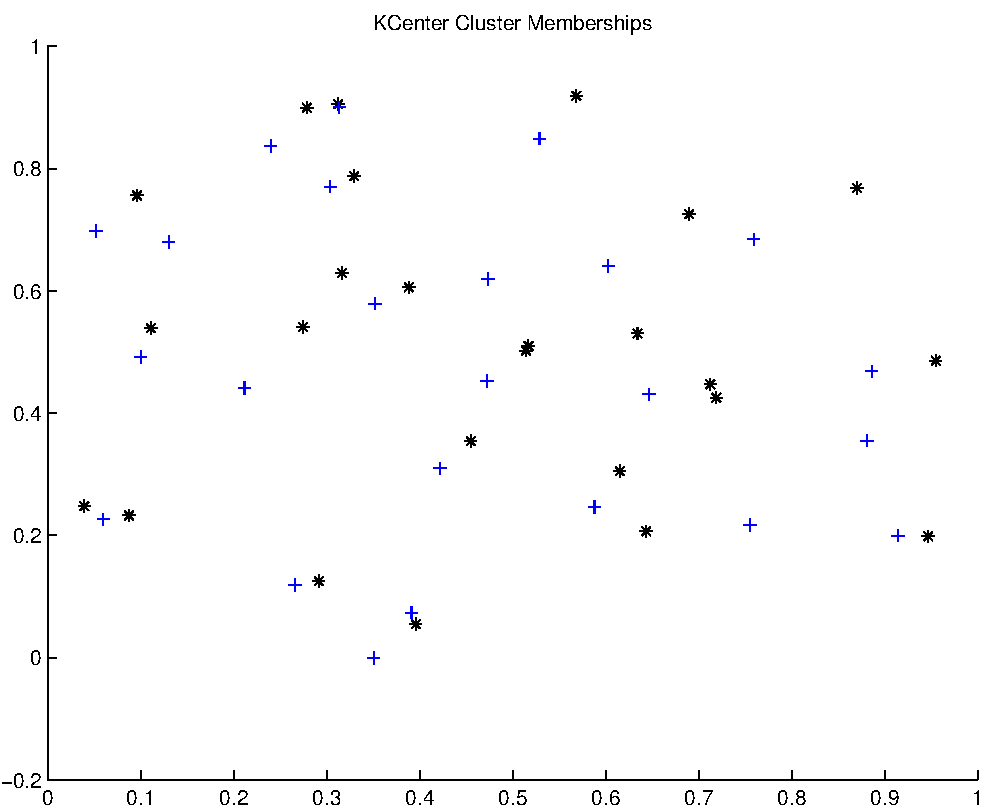
\includegraphics[width=10.0cm,height=10.0cm]{KCenterClusterMemberships_25_Centers.pdf}

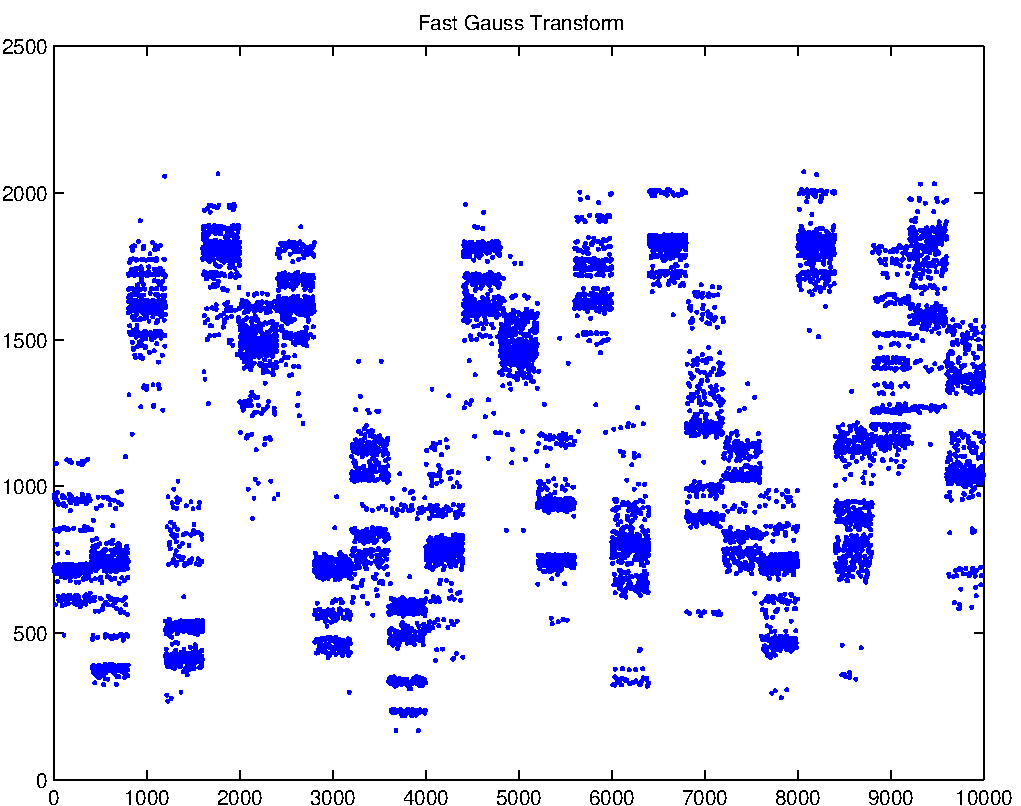
\includegraphics[width=10.0cm,height=10.0cm]{FGT25_Centers.pdf}

QueryPerformanceCounter  =  +7.292
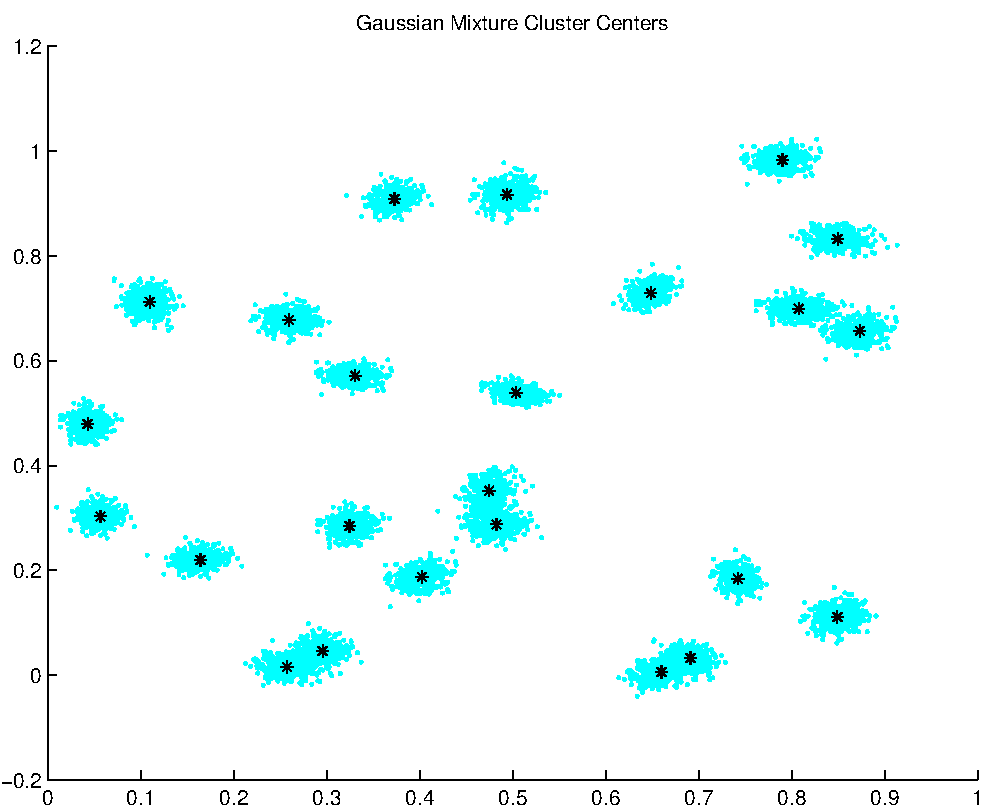
\includegraphics[width=10.0cm,height=10.0cm]{GaussianMixture_ClusterCenters24_Centers.pdf}

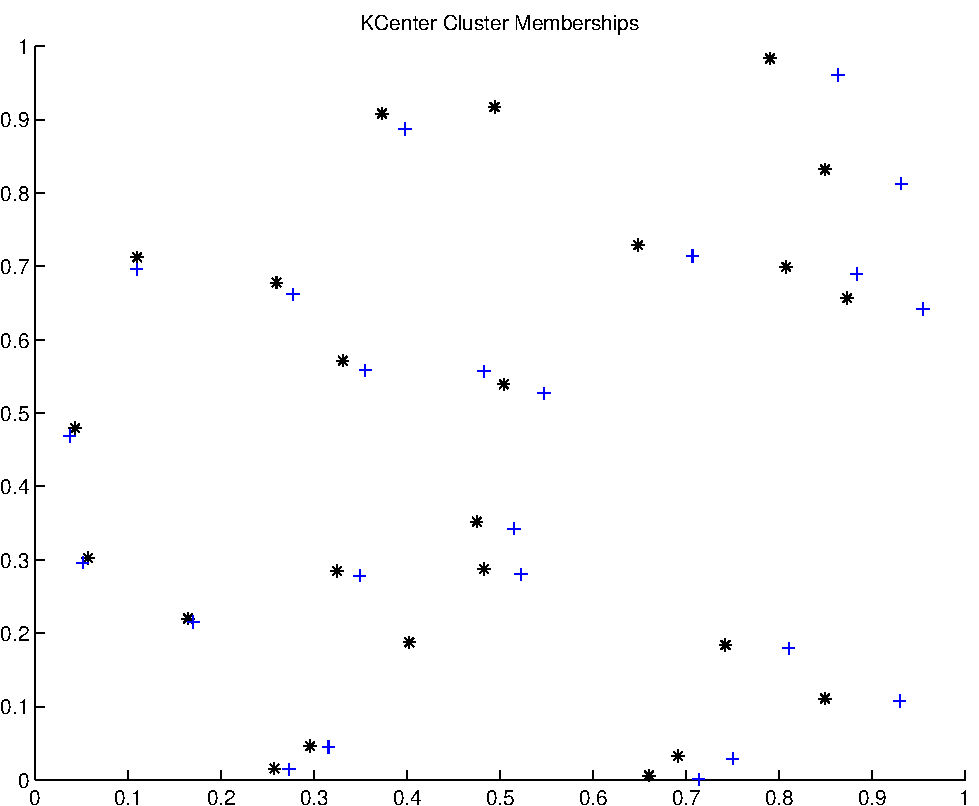
\includegraphics[width=10.0cm,height=10.0cm]{KCenterClusterMemberships_24_Centers.pdf}

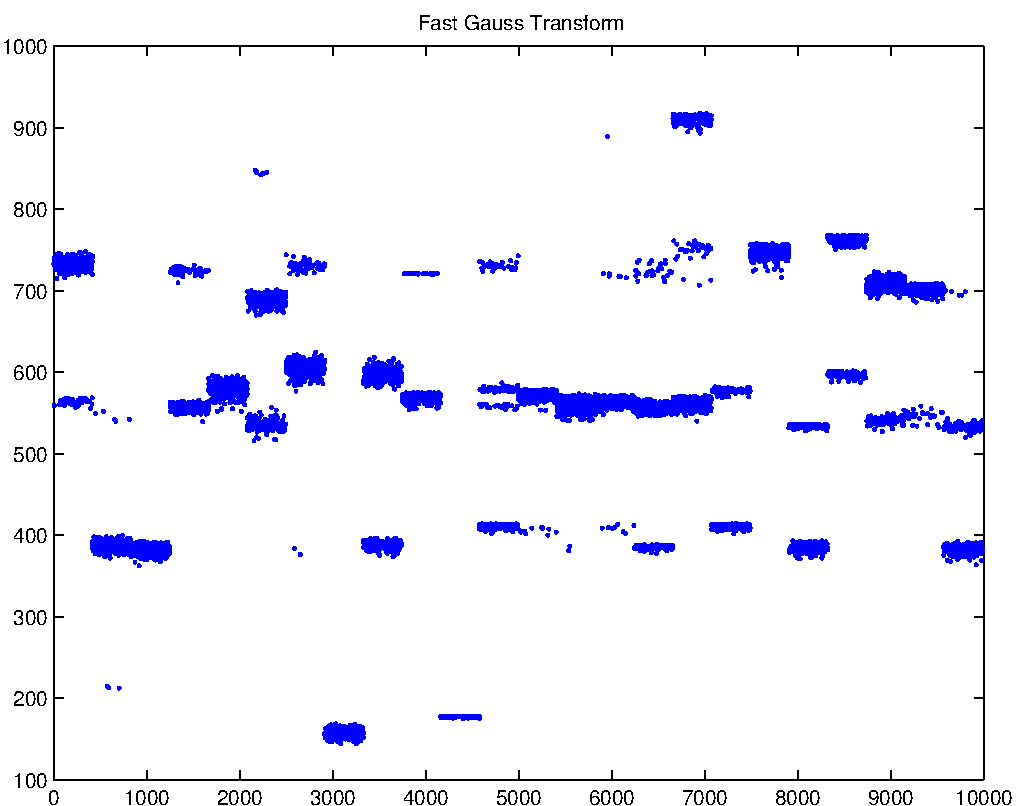
\includegraphics[width=10.0cm,height=10.0cm]{FGT24_Centers.pdf}

QueryPerformanceCounter  =  +7.402
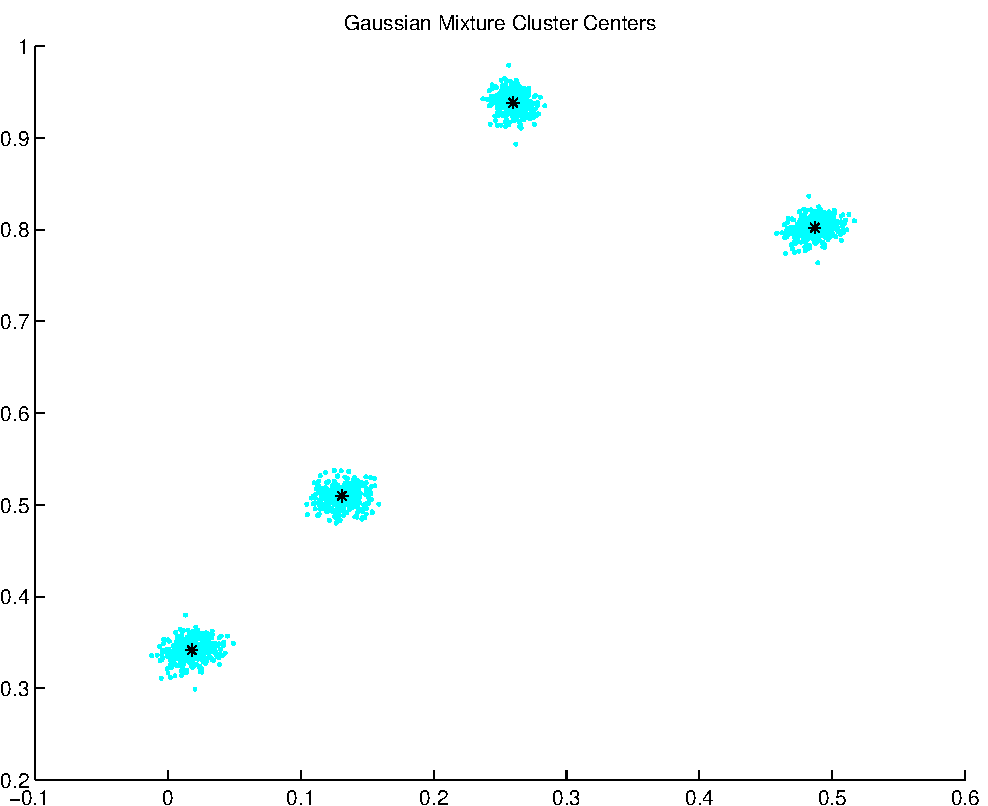
\includegraphics[width=10.0cm,height=10.0cm]{GaussianMixture_ClusterCenters4_Centers.pdf}

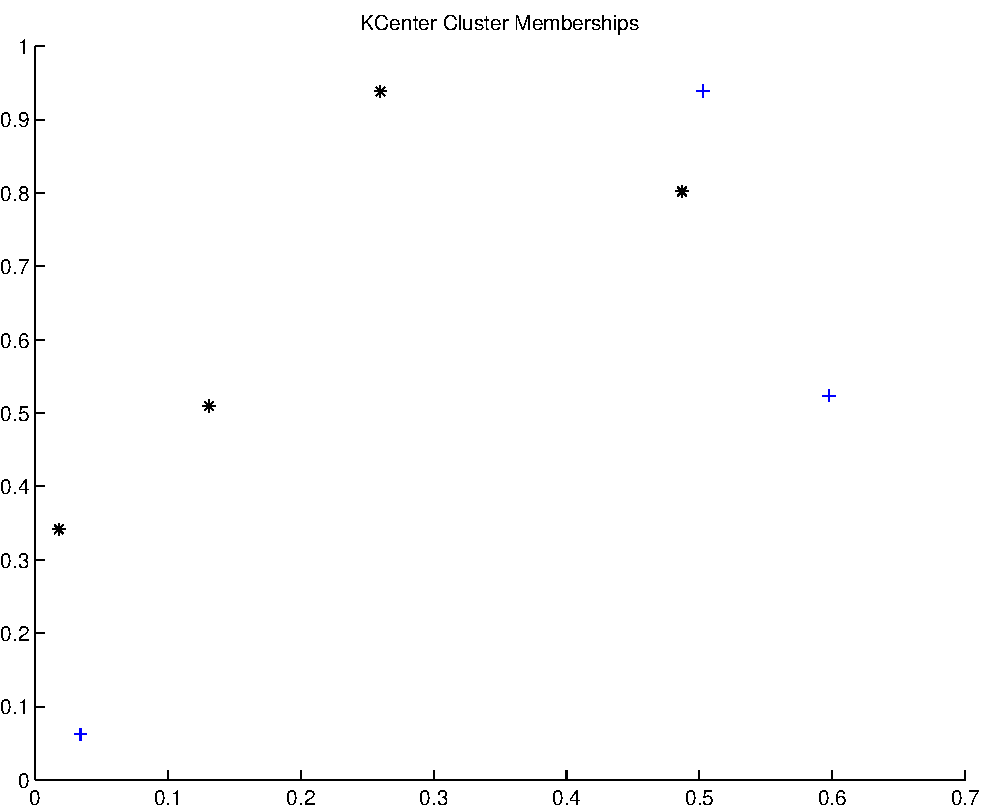
\includegraphics[width=10.0cm,height=10.0cm]{KCenterClusterMemberships_4_Centers.pdf}

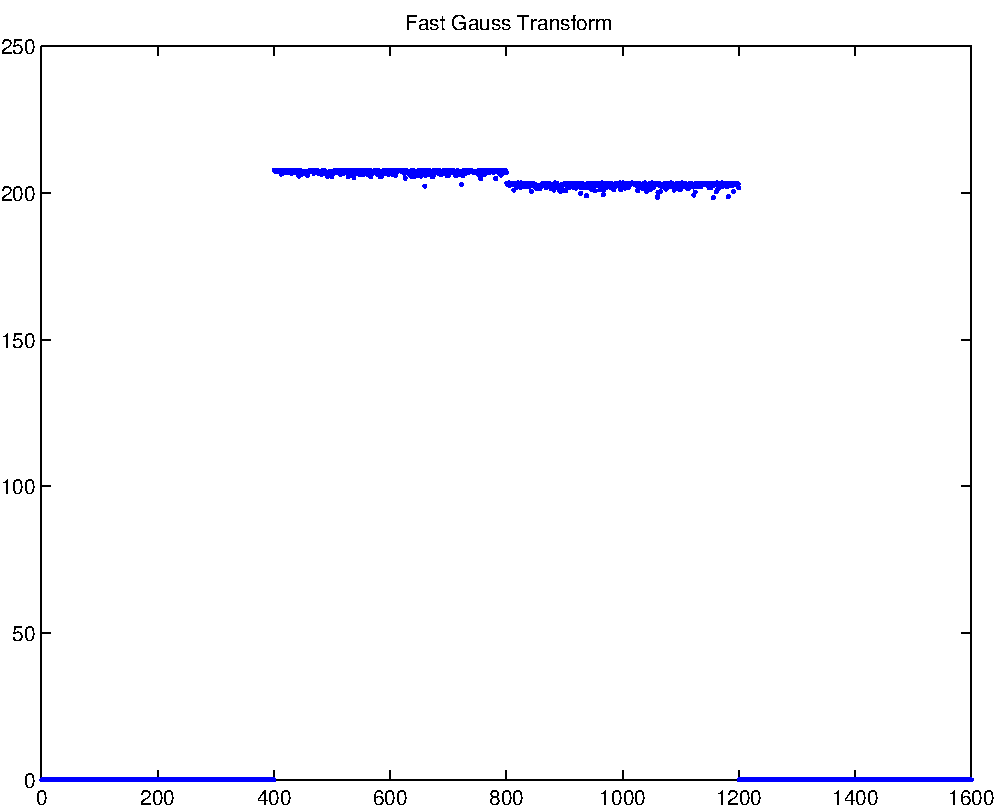
\includegraphics[width=10.0cm,height=10.0cm]{FGT4_Centers.pdf}

QueryPerformanceCounter  =  +3.376
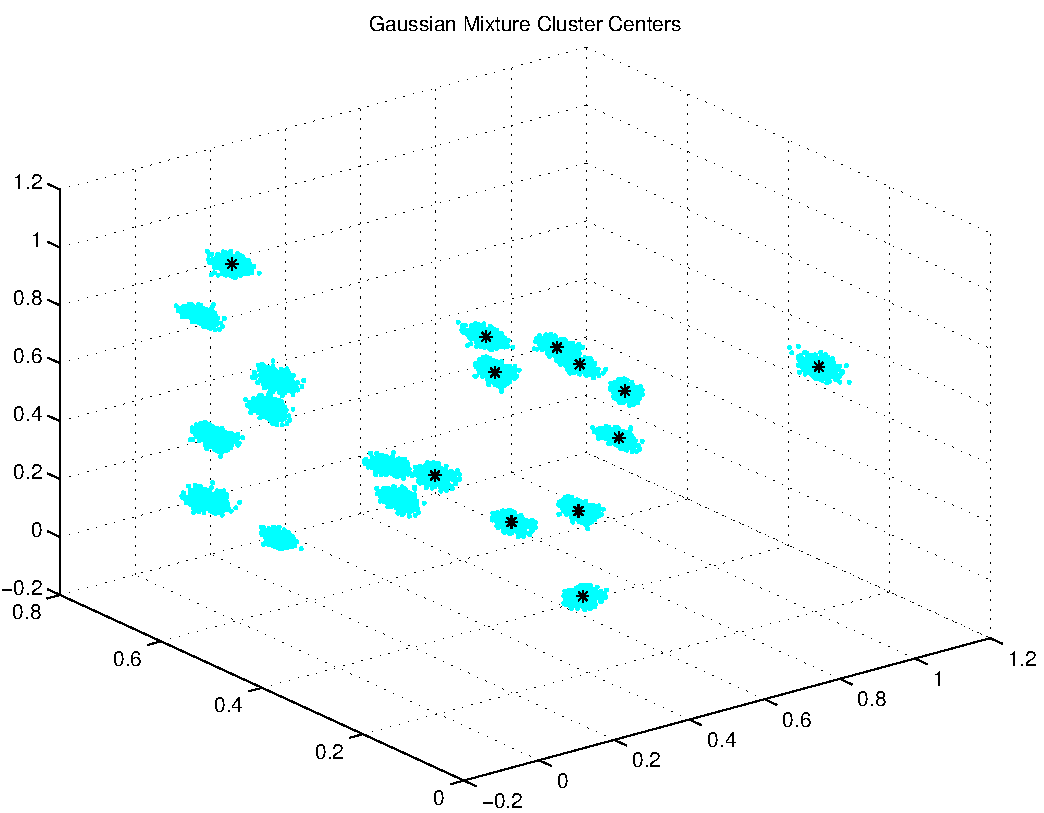
\includegraphics[width=10.0cm,height=10.0cm]{GaussianMixture_ClusterCenters20_Centers.pdf}

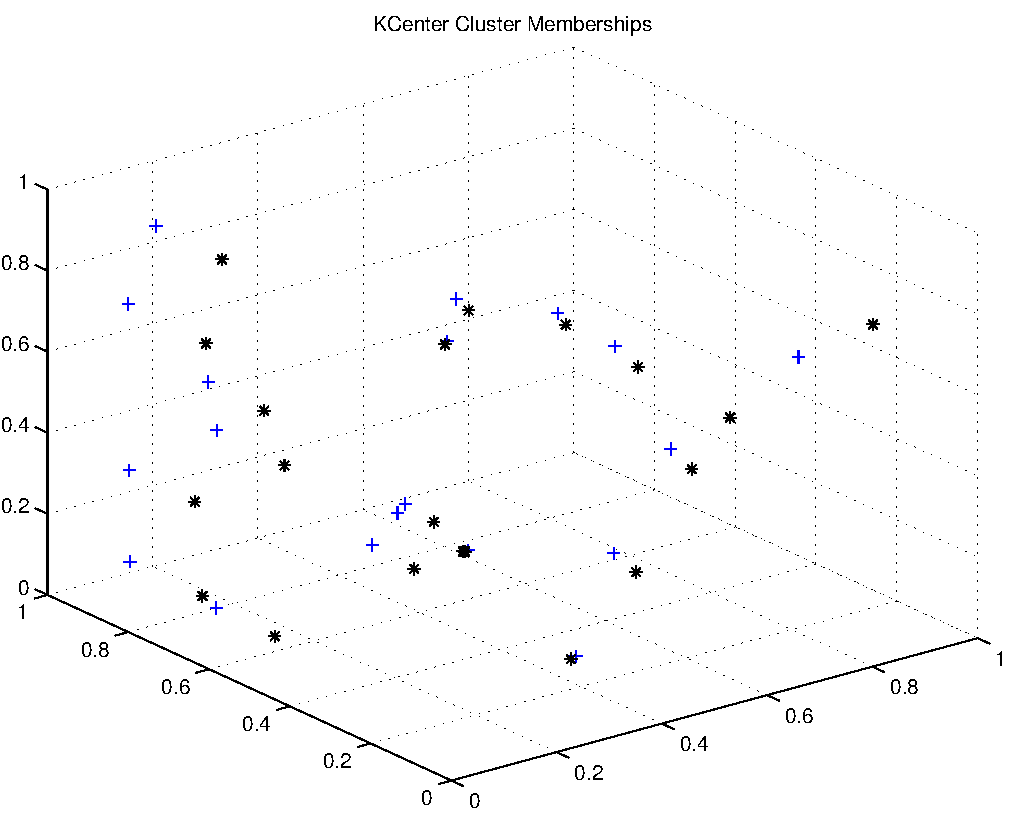
\includegraphics[width=10.0cm,height=10.0cm]{KCenterClusterMemberships_20_Centers.pdf}

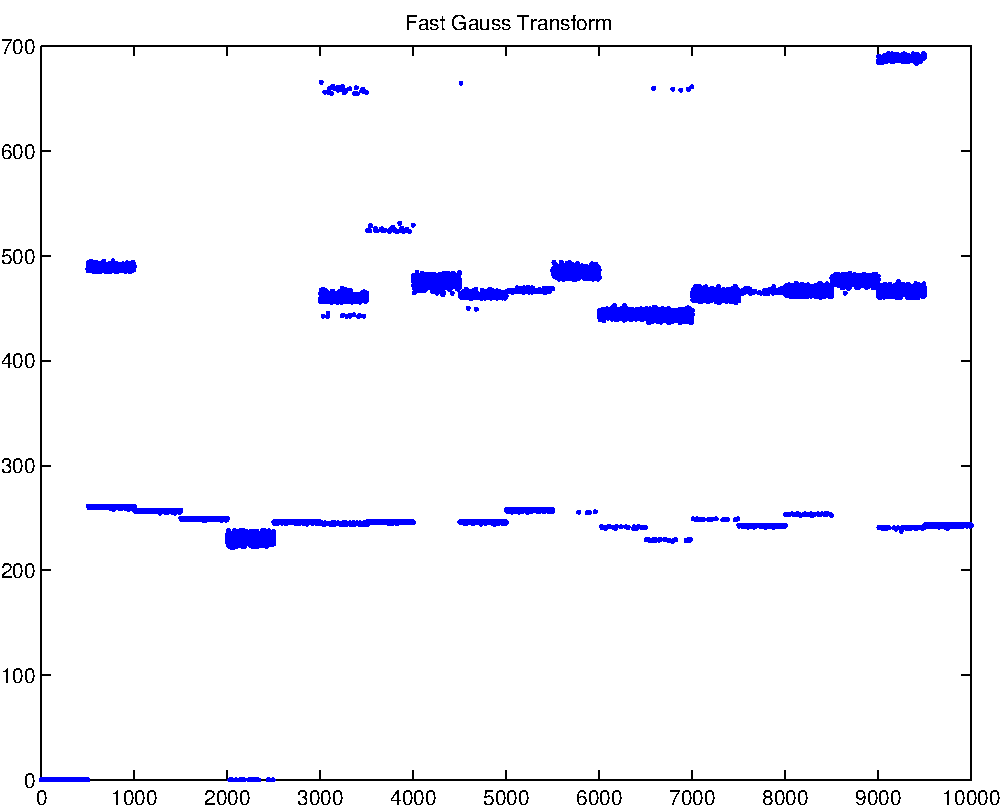
\includegraphics[width=10.0cm,height=10.0cm]{FGT20_Centers.pdf}

QueryPerformanceCounter  =  +5.523
\subsubsection{Matrix Norms}
\subsubsection{Haar Distributed Random Orthogonal Matrix $A \in O(n)$}
 Testing Operator Norm
Number of Dimensions: +12

$A = \left(
\begin{array}{
cccccccccccc}
+0.222 & +0.588 & +0.234 & +0.102 & -0.140 & +0.073 & +0.199 & +0.394 & +0.050 & -0.128 & +0.318 & -0.448 \\
+0.096 & -0.002 & -0.280 & -0.139 & +0.312 & -0.031 & +0.219 & -0.405 & -0.040 & -0.039 & +0.760 & +0.052 \\
-0.455 & +0.046 & +0.438 & -0.161 & +0.153 & -0.463 & +0.060 & -0.334 & +0.234 & +0.087 & -0.043 & -0.393 \\
+0.011 & +0.158 & +0.043 & +0.001 & +0.567 & -0.067 & -0.296 & +0.382 & +0.074 & +0.613 & +0.093 & +0.152 \\
+0.282 & -0.430 & +0.049 & -0.026 & -0.082 & +0.446 & -0.176 & -0.147 & +0.319 & +0.313 & +0.070 & -0.519 \\
+0.078 & -0.350 & +0.186 & +0.564 & -0.024 & -0.364 & -0.411 & +0.092 & -0.261 & -0.187 & +0.307 & -0.107 \\
+0.226 & -0.131 & +0.315 & -0.736 & -0.089 & -0.071 & -0.235 & +0.125 & -0.439 & -0.069 & +0.094 & -0.004 \\
-0.311 & -0.516 & -0.022 & -0.080 & -0.067 & -0.059 & +0.525 & +0.550 & +0.039 & +0.077 & +0.190 & -0.016 \\
-0.295 & -0.015 & +0.418 & -0.034 & +0.045 & +0.421 & -0.249 & +0.061 & +0.392 & -0.356 & +0.265 & +0.376 \\
-0.244 & +0.155 & -0.271 & -0.117 & -0.671 & -0.200 & -0.313 & +0.019 & +0.184 & +0.327 & +0.297 & +0.106 \\
+0.591 & -0.105 & +0.155 & -0.055 & -0.078 & -0.436 & +0.156 & +0.020 & +0.542 & -0.043 & -0.043 & +0.307 \\
-0.066 & -0.030 & -0.514 & -0.244 & +0.244 & -0.165 & -0.324 & +0.265 & +0.300 & -0.469 & -0.085 & -0.302 \\
\end{array}
\right)$ \newline 

$Det(A) :   A \in O(n)$ = (+1.000,+0.000)

$L = \left(
\begin{array}{
cccccccccccc}
+1.000 & +0.000 & +0.000 & +0.000 & +0.000 & +0.000 & +0.000 & +0.000 & +0.000 & +0.000 & +0.000 & +0.000 \\
+0.375 & +1.000 & +0.000 & +0.000 & +0.000 & +0.000 & +0.000 & +0.000 & +0.000 & +0.000 & +0.000 & +0.000 \\
-0.770 & -0.056 & +1.000 & +0.000 & +0.000 & +0.000 & +0.000 & +0.000 & +0.000 & +0.000 & +0.000 & +0.000 \\
+0.132 & -0.535 & +0.457 & +1.000 & +0.000 & +0.000 & +0.000 & +0.000 & +0.000 & +0.000 & +0.000 & +0.000 \\
-0.413 & +0.177 & -0.420 & -0.336 & +1.000 & +0.000 & +0.000 & +0.000 & +0.000 & +0.000 & +0.000 & +0.000 \\
-0.111 & -0.067 & -0.855 & -0.565 & -0.348 & +1.000 & +0.000 & +0.000 & +0.000 & +0.000 & +0.000 & +0.000 \\
+0.382 & -0.145 & +0.495 & -0.827 & +0.308 & -0.872 & +1.000 & +0.000 & +0.000 & +0.000 & +0.000 & +0.000 \\
-0.525 & -0.911 & +0.387 & +0.109 & +0.335 & -0.440 & -0.563 & +1.000 & +0.000 & +0.000 & +0.000 & +0.000 \\
-0.499 & -0.107 & +0.906 & +0.179 & +0.094 & -0.964 & +0.658 & -0.022 & +1.000 & +0.000 & +0.000 & +0.000 \\
+0.019 & +0.255 & -0.008 & -0.043 & -0.865 & +0.709 & +0.271 & -0.101 & +0.178 & +1.000 & +0.000 & +0.000 \\
+0.163 & +0.025 & -0.545 & -0.330 & -0.493 & +0.670 & -0.296 & -0.221 & -0.439 & -0.148 & +1.000 & +0.000 \\
+0.477 & -0.606 & +0.143 & +0.141 & +0.159 & -0.985 & +0.537 & -0.099 & +0.733 & +0.279 & +0.101 & +1.000 \\
\end{array}
\right)$ \newline 

$U = \left(
\begin{array}{
cccccccccccc}
+0.591 & -0.105 & +0.155 & -0.055 & -0.078 & -0.436 & +0.156 & +0.020 & +0.542 & -0.043 & -0.043 & +0.307 \\
+0.000 & +0.627 & +0.176 & +0.122 & -0.110 & +0.237 & +0.140 & +0.386 & -0.153 & -0.112 & +0.334 & -0.563 \\
+0.000 & +0.000 & +0.568 & -0.196 & +0.087 & -0.786 & +0.188 & -0.296 & +0.642 & +0.048 & -0.057 & -0.189 \\
+0.000 & +0.000 & +0.000 & +0.726 & -0.112 & +0.179 & -0.443 & +0.431 & -0.708 & -0.263 & +0.517 & -0.362 \\
+0.000 & +0.000 & +0.000 & +0.000 & -0.685 & -0.692 & -0.344 & -0.021 & +0.467 & +0.261 & +0.370 & +0.131 \\
+0.000 & +0.000 & +0.000 & +0.000 & +0.000 & -1.010 & -0.507 & +0.276 & +0.662 & -0.498 & +0.305 & -0.626 \\
+0.000 & +0.000 & +0.000 & +0.000 & +0.000 & +0.000 & -1.070 & +0.923 & -1.139 & -0.825 & +0.767 & -0.994 \\
+0.000 & +0.000 & +0.000 & +0.000 & +0.000 & +0.000 & +0.000 & +1.629 & -0.494 & -0.808 & +0.879 & -1.134 \\
+0.000 & +0.000 & +0.000 & +0.000 & +0.000 & +0.000 & +0.000 & +0.000 & +1.523 & -0.365 & +0.013 & +0.719 \\
+0.000 & +0.000 & +0.000 & +0.000 & +0.000 & +0.000 & +0.000 & +0.000 & +0.000 & +1.417 & +0.013 & +0.857 \\
+0.000 & +0.000 & +0.000 & +0.000 & +0.000 & +0.000 & +0.000 & +0.000 & +0.000 & +0.000 & +1.304 & +0.175 \\
+0.000 & +0.000 & +0.000 & +0.000 & +0.000 & +0.000 & +0.000 & +0.000 & +0.000 & +0.000 & +0.000 & -1.927 \\
\end{array}
\right)$ \newline 

$L * U  = \left(
\begin{array}{
cccccccccccc}
+0.591 & -0.105 & +0.155 & -0.055 & -0.078 & -0.436 & +0.156 & +0.020 & +0.542 & -0.043 & -0.043 & +0.307 \\
+0.222 & +0.588 & +0.234 & +0.102 & -0.140 & +0.073 & +0.199 & +0.394 & +0.050 & -0.128 & +0.318 & -0.448 \\
-0.455 & +0.046 & +0.438 & -0.161 & +0.153 & -0.463 & +0.060 & -0.334 & +0.234 & +0.087 & -0.043 & -0.393 \\
+0.078 & -0.350 & +0.186 & +0.564 & -0.024 & -0.364 & -0.411 & +0.092 & -0.261 & -0.187 & +0.307 & -0.107 \\
-0.244 & +0.155 & -0.271 & -0.117 & -0.671 & -0.200 & -0.313 & +0.019 & +0.184 & +0.327 & +0.297 & +0.106 \\
-0.066 & -0.030 & -0.514 & -0.244 & +0.244 & -0.165 & -0.324 & +0.265 & +0.300 & -0.469 & -0.085 & -0.302 \\
+0.226 & -0.131 & +0.315 & -0.736 & -0.089 & -0.071 & -0.235 & +0.125 & -0.439 & -0.069 & +0.094 & -0.004 \\
-0.311 & -0.516 & -0.022 & -0.080 & -0.067 & -0.059 & +0.525 & +0.550 & +0.039 & +0.077 & +0.190 & -0.016 \\
-0.295 & -0.015 & +0.418 & -0.034 & +0.045 & +0.421 & -0.249 & +0.061 & +0.392 & -0.356 & +0.265 & +0.376 \\
+0.011 & +0.158 & +0.043 & +0.001 & +0.567 & -0.067 & -0.296 & +0.382 & +0.074 & +0.613 & +0.093 & +0.152 \\
+0.096 & -0.002 & -0.280 & -0.139 & +0.312 & -0.031 & +0.219 & -0.405 & -0.040 & -0.039 & +0.760 & +0.052 \\
+0.282 & -0.430 & +0.049 & -0.026 & -0.082 & +0.446 & -0.176 & -0.147 & +0.319 & +0.313 & +0.070 & -0.519 \\
\end{array}
\right)$ \newline 

$Det(L) :    = (+1.000,+0.000)     Det(U) :    = (+1.000,+0.000)     Det(LU) :    = (+1.000,+0.000)$

$||A||_{L_1}$  = +3.165

$||A||_{L_{\infty}}$ = +3.009

$||A^{-1}||_{L_1}$  = +3.009

$||A^{-1}||_{L_{\infty}}$ = +3.165

$||A||_{L_{\infty}} * ||A^{-1}||_{L_{\infty}} = +9.522$

$||A||_{L_1} * ||A^{-1}||_{L_1} = +9.522$

Frobenious Norm  $||A||_{\textit{F}}$ via $\sum\limits_{i,j =0}^{n} \|A_{i,j}|$   of  $A \in O(n)$  +3.464

$L_1$ condition number of Haar Distributed Random Orthogonal Matrix $A \in O(n)$ +7.780

$A = \left(
\begin{array}{
cccccccccccc}
+0.222 & +0.588 & +0.234 & +0.102 & -0.140 & +0.073 & +0.199 & +0.394 & +0.050 & -0.128 & +0.318 & -0.448 \\
+0.096 & -0.002 & -0.280 & -0.139 & +0.312 & -0.031 & +0.219 & -0.405 & -0.040 & -0.039 & +0.760 & +0.052 \\
-0.455 & +0.046 & +0.438 & -0.161 & +0.153 & -0.463 & +0.060 & -0.334 & +0.234 & +0.087 & -0.043 & -0.393 \\
+0.011 & +0.158 & +0.043 & +0.001 & +0.567 & -0.067 & -0.296 & +0.382 & +0.074 & +0.613 & +0.093 & +0.152 \\
+0.282 & -0.430 & +0.049 & -0.026 & -0.082 & +0.446 & -0.176 & -0.147 & +0.319 & +0.313 & +0.070 & -0.519 \\
+0.078 & -0.350 & +0.186 & +0.564 & -0.024 & -0.364 & -0.411 & +0.092 & -0.261 & -0.187 & +0.307 & -0.107 \\
+0.226 & -0.131 & +0.315 & -0.736 & -0.089 & -0.071 & -0.235 & +0.125 & -0.439 & -0.069 & +0.094 & -0.004 \\
-0.311 & -0.516 & -0.022 & -0.080 & -0.067 & -0.059 & +0.525 & +0.550 & +0.039 & +0.077 & +0.190 & -0.016 \\
-0.295 & -0.015 & +0.418 & -0.034 & +0.045 & +0.421 & -0.249 & +0.061 & +0.392 & -0.356 & +0.265 & +0.376 \\
-0.244 & +0.155 & -0.271 & -0.117 & -0.671 & -0.200 & -0.313 & +0.019 & +0.184 & +0.327 & +0.297 & +0.106 \\
+0.591 & -0.105 & +0.155 & -0.055 & -0.078 & -0.436 & +0.156 & +0.020 & +0.542 & -0.043 & -0.043 & +0.307 \\
-0.066 & -0.030 & -0.514 & -0.244 & +0.244 & -0.165 & -0.324 & +0.265 & +0.300 & -0.469 & -0.085 & -0.302 \\
\end{array}
\right)$ \newline 

$L_{\infty}$ condition number of Haar Distributed Random Orthogonal Matrix $A \in O(n)$ +8.412

Eigenvalues of $A \in O(n)$

(-0.917,+0.400), (-0.917,-0.400), (-0.622,+0.783), (-0.622,-0.783), (-0.363,+0.932), (-0.363,-0.932), (+0.535,+0.845), (+0.535,-0.845), (+0.822,+0.570), (+0.822,-0.570), (+0.996,+0.092), (+0.996,-0.092)

 $|\lambda | : \lambda \in \sigma(A) , A \in O(n)$

+1.000, +1.000, +1.000, +1.000, +1.000, +1.000, +1.000, +1.000, +1.000, +1.000, +1.000, +1.000


Calculating $A^{\dag} A,$  we expect $A^{\dag} A \approx I$

$A^{\dag} A = \left(
\begin{array}{
cccccccccccc}
+1.000 & +0.000 & +0.000 & -0.000 & -0.000 & +0.000 & -0.000 & +0.000 & -0.000 & +0.000 & -0.000 & -0.000 \\
+0.000 & +1.000 & -0.000 & +0.000 & +0.000 & -0.000 & -0.000 & -0.000 & -0.000 & -0.000 & +0.000 & -0.000 \\
+0.000 & -0.000 & +1.000 & -0.000 & +0.000 & -0.000 & +0.000 & -0.000 & -0.000 & +0.000 & +0.000 & +0.000 \\
-0.000 & +0.000 & -0.000 & +1.000 & +0.000 & +0.000 & +0.000 & +0.000 & +0.000 & +0.000 & -0.000 & +0.000 \\
-0.000 & +0.000 & +0.000 & +0.000 & +1.000 & -0.000 & -0.000 & -0.000 & -0.000 & -0.000 & -0.000 & -0.000 \\
+0.000 & -0.000 & -0.000 & +0.000 & -0.000 & +1.000 & -0.000 & +0.000 & +0.000 & +0.000 & +0.000 & -0.000 \\
-0.000 & -0.000 & +0.000 & +0.000 & -0.000 & -0.000 & +1.000 & +0.000 & -0.000 & +0.000 & -0.000 & +0.000 \\
+0.000 & -0.000 & -0.000 & +0.000 & -0.000 & +0.000 & +0.000 & +1.000 & -0.000 & -0.000 & +0.000 & -0.000 \\
-0.000 & -0.000 & -0.000 & +0.000 & -0.000 & +0.000 & -0.000 & -0.000 & +1.000 & -0.000 & +0.000 & -0.000 \\
+0.000 & -0.000 & +0.000 & +0.000 & -0.000 & +0.000 & +0.000 & -0.000 & -0.000 & +1.000 & +0.000 & +0.000 \\
-0.000 & +0.000 & +0.000 & -0.000 & -0.000 & +0.000 & -0.000 & +0.000 & +0.000 & +0.000 & +1.000 & +0.000 \\
-0.000 & -0.000 & +0.000 & +0.000 & -0.000 & -0.000 & +0.000 & -0.000 & -0.000 & +0.000 & +0.000 & +1.000 \\
\end{array}
\right)$ \newline 

Calculating $A^{-1} ,  A \in O(n)$.

$A^{-1} = \left(
\begin{array}{
cccccccccccc}
+0.222 & +0.096 & -0.455 & +0.011 & +0.282 & +0.078 & +0.226 & -0.311 & -0.295 & -0.244 & +0.591 & -0.066 \\
+0.588 & -0.002 & +0.046 & +0.158 & -0.430 & -0.350 & -0.131 & -0.516 & -0.015 & +0.155 & -0.105 & -0.030 \\
+0.234 & -0.280 & +0.438 & +0.043 & +0.049 & +0.186 & +0.315 & -0.022 & +0.418 & -0.271 & +0.155 & -0.514 \\
+0.102 & -0.139 & -0.161 & +0.001 & -0.026 & +0.564 & -0.736 & -0.080 & -0.034 & -0.117 & -0.055 & -0.244 \\
-0.140 & +0.312 & +0.153 & +0.567 & -0.082 & -0.024 & -0.089 & -0.067 & +0.045 & -0.671 & -0.078 & +0.244 \\
+0.073 & -0.031 & -0.463 & -0.067 & +0.446 & -0.364 & -0.071 & -0.059 & +0.421 & -0.200 & -0.436 & -0.165 \\
+0.199 & +0.219 & +0.060 & -0.296 & -0.176 & -0.411 & -0.235 & +0.525 & -0.249 & -0.313 & +0.156 & -0.324 \\
+0.394 & -0.405 & -0.334 & +0.382 & -0.147 & +0.092 & +0.125 & +0.550 & +0.061 & +0.019 & +0.020 & +0.265 \\
+0.050 & -0.040 & +0.234 & +0.074 & +0.319 & -0.261 & -0.439 & +0.039 & +0.392 & +0.184 & +0.542 & +0.300 \\
-0.128 & -0.039 & +0.087 & +0.613 & +0.313 & -0.187 & -0.069 & +0.077 & -0.356 & +0.327 & -0.043 & -0.469 \\
+0.318 & +0.760 & -0.043 & +0.093 & +0.070 & +0.307 & +0.094 & +0.190 & +0.265 & +0.297 & -0.043 & -0.085 \\
-0.448 & +0.052 & -0.393 & +0.152 & -0.519 & -0.107 & -0.004 & -0.016 & +0.376 & +0.106 & +0.307 & -0.302 \\
\end{array}
\right)$ \newline 

Calculating $A^{-1} *A  ,  A \in O(n)$.   We expect $A^{-1} *A  \approx I$. 

$A^{-1} *A = \left(
\begin{array}{
cccccccccccc}
+1.000 & +0.000 & +0.000 & +0.000 & +0.000 & +0.000 & -0.000 & +0.000 & -0.000 & +0.000 & +0.000 & -0.000 \\
+0.000 & +1.000 & +0.000 & +0.000 & -0.000 & -0.000 & +0.000 & +0.000 & +0.000 & -0.000 & +0.000 & -0.000 \\
+0.000 & -0.000 & +1.000 & +0.000 & +0.000 & +0.000 & -0.000 & +0.000 & +0.000 & -0.000 & +0.000 & -0.000 \\
+0.000 & +0.000 & -0.000 & +1.000 & +0.000 & -0.000 & -0.000 & +0.000 & -0.000 & -0.000 & -0.000 & -0.000 \\
+0.000 & -0.000 & +0.000 & -0.000 & +1.000 & +0.000 & +0.000 & -0.000 & -0.000 & +0.000 & -0.000 & +0.000 \\
-0.000 & +0.000 & -0.000 & +0.000 & +0.000 & +1.000 & +0.000 & -0.000 & -0.000 & +0.000 & -0.000 & +0.000 \\
-0.000 & -0.000 & +0.000 & -0.000 & -0.000 & -0.000 & +1.000 & -0.000 & +0.000 & +0.000 & +0.000 & -0.000 \\
+0.000 & -0.000 & +0.000 & -0.000 & +0.000 & -0.000 & +0.000 & +1.000 & +0.000 & -0.000 & -0.000 & +0.000 \\
+0.000 & -0.000 & +0.000 & +0.000 & -0.000 & -0.000 & +0.000 & -0.000 & +1.000 & +0.000 & -0.000 & +0.000 \\
-0.000 & -0.000 & -0.000 & -0.000 & +0.000 & +0.000 & +0.000 & -0.000 & +0.000 & +1.000 & -0.000 & -0.000 \\
-0.000 & -0.000 & +0.000 & -0.000 & +0.000 & +0.000 & -0.000 & -0.000 & -0.000 & +0.000 & +1.000 & +0.000 \\
-0.000 & +0.000 & +0.000 & -0.000 & +0.000 & -0.000 & -0.000 & +0.000 & +0.000 & +0.000 & +0.000 & +1.000 \\
\end{array}
\right)$ \newline 

Calculating SVD of  $A \in O(n)$

$U = \left(
\begin{array}{
cccccccccccc}
-0.233 & -0.060 & +0.220 & +0.453 & +0.132 & +0.038 & -0.146 & -0.479 & +0.316 & -0.357 & -0.094 & -0.428 \\
+0.206 & -0.442 & +0.175 & -0.563 & -0.035 & +0.377 & +0.018 & +0.091 & +0.434 & -0.158 & +0.078 & -0.206 \\
+0.057 & +0.222 & -0.065 & -0.503 & +0.418 & -0.353 & -0.121 & -0.309 & -0.136 & +0.249 & -0.027 & -0.447 \\
+0.867 & +0.034 & +0.086 & +0.151 & +0.148 & -0.147 & -0.064 & -0.169 & +0.025 & -0.218 & -0.214 & +0.218 \\
+0.114 & -0.103 & +0.370 & +0.273 & +0.220 & +0.166 & -0.388 & +0.081 & +0.134 & +0.667 & +0.258 & +0.041 \\
+0.087 & -0.319 & +0.462 & +0.046 & -0.320 & -0.015 & +0.369 & -0.152 & -0.501 & +0.206 & -0.220 & -0.267 \\
+0.054 & +0.206 & -0.089 & -0.016 & -0.101 & +0.130 & +0.565 & -0.541 & +0.329 & +0.294 & +0.259 & +0.212 \\
-0.222 & -0.588 & -0.234 & -0.102 & +0.140 & -0.073 & -0.199 & -0.394 & -0.050 & +0.128 & -0.318 & +0.448 \\
-0.245 & +0.031 & +0.558 & -0.102 & +0.483 & -0.271 & +0.344 & +0.194 & +0.121 & -0.159 & -0.058 & +0.333 \\
-0.086 & +0.206 & +0.403 & -0.285 & -0.465 & -0.180 & -0.427 & -0.292 & -0.067 & -0.184 & +0.271 & +0.280 \\
-0.001 & +0.048 & +0.015 & -0.036 & +0.392 & +0.577 & -0.004 & -0.194 & -0.536 & -0.261 & +0.323 & +0.105 \\
+0.092 & -0.452 & -0.150 & +0.145 & +0.042 & -0.470 & +0.111 & +0.025 & -0.072 & -0.144 & +0.688 & -0.090 \\
\end{array}
\right)$ \newline 

$S = \left(
\begin{array}{
cccccccccccc}
+1.000 & +0.000 & +0.000 & +0.000 & +0.000 & +0.000 & +0.000 & +0.000 & +0.000 & +0.000 & +0.000 & +0.000 \\
+0.000 & +1.000 & +0.000 & +0.000 & +0.000 & +0.000 & +0.000 & +0.000 & +0.000 & +0.000 & +0.000 & +0.000 \\
+0.000 & +0.000 & +1.000 & +0.000 & +0.000 & +0.000 & +0.000 & +0.000 & +0.000 & +0.000 & +0.000 & +0.000 \\
+0.000 & +0.000 & +0.000 & +1.000 & +0.000 & +0.000 & +0.000 & +0.000 & +0.000 & +0.000 & +0.000 & +0.000 \\
+0.000 & +0.000 & +0.000 & +0.000 & +1.000 & +0.000 & +0.000 & +0.000 & +0.000 & +0.000 & +0.000 & +0.000 \\
+0.000 & +0.000 & +0.000 & +0.000 & +0.000 & +1.000 & +0.000 & +0.000 & +0.000 & +0.000 & +0.000 & +0.000 \\
+0.000 & +0.000 & +0.000 & +0.000 & +0.000 & +0.000 & +1.000 & +0.000 & +0.000 & +0.000 & +0.000 & +0.000 \\
+0.000 & +0.000 & +0.000 & +0.000 & +0.000 & +0.000 & +0.000 & +1.000 & +0.000 & +0.000 & +0.000 & +0.000 \\
+0.000 & +0.000 & +0.000 & +0.000 & +0.000 & +0.000 & +0.000 & +0.000 & +1.000 & +0.000 & +0.000 & +0.000 \\
+0.000 & +0.000 & +0.000 & +0.000 & +0.000 & +0.000 & +0.000 & +0.000 & +0.000 & +1.000 & +0.000 & +0.000 \\
+0.000 & +0.000 & +0.000 & +0.000 & +0.000 & +0.000 & +0.000 & +0.000 & +0.000 & +0.000 & +1.000 & +0.000 \\
+0.000 & +0.000 & +0.000 & +0.000 & +0.000 & +0.000 & +0.000 & +0.000 & +0.000 & +0.000 & +0.000 & +1.000 \\
\end{array}
\right)$ \newline 

$V = \left(
\begin{array}{
cccccccccccc}
-0.000 & -0.000 & +0.000 & +0.000 & +0.000 & -0.000 & -0.000 & -1.000 & -0.000 & -0.000 & +0.000 & +0.000 \\
-0.038 & +0.031 & +0.285 & +0.000 & -0.017 & -0.252 & +0.523 & -0.000 & -0.035 & +0.034 & +0.466 & +0.600 \\
+0.495 & +0.010 & +0.527 & -0.326 & +0.030 & +0.187 & +0.095 & -0.000 & +0.415 & +0.201 & -0.332 & +0.048 \\
-0.339 & -0.165 & +0.283 & -0.051 & +0.710 & -0.349 & -0.149 & -0.000 & +0.247 & -0.238 & -0.036 & -0.088 \\
+0.266 & +0.628 & +0.071 & +0.000 & +0.448 & +0.187 & +0.074 & +0.000 & -0.490 & -0.215 & -0.050 & +0.000 \\
+0.299 & -0.288 & -0.200 & +0.163 & +0.284 & +0.131 & -0.505 & +0.000 & -0.076 & +0.166 & +0.007 & +0.612 \\
-0.471 & +0.386 & +0.353 & +0.081 & -0.056 & +0.284 & -0.373 & +0.000 & +0.061 & +0.476 & +0.209 & +0.040 \\
-0.315 & +0.268 & -0.315 & -0.489 & -0.091 & +0.215 & -0.040 & +0.000 & +0.304 & -0.379 & -0.172 & +0.412 \\
+0.240 & +0.365 & -0.466 & -0.163 & +0.194 & -0.380 & -0.007 & +0.000 & +0.356 & +0.409 & +0.265 & -0.139 \\
-0.256 & -0.127 & -0.080 & -0.407 & +0.089 & -0.221 & +0.155 & +0.000 & -0.461 & +0.491 & -0.450 & +0.096 \\
-0.122 & +0.245 & -0.096 & +0.652 & +0.018 & -0.112 & +0.245 & +0.000 & +0.259 & +0.094 & -0.549 & +0.201 \\
+0.139 & +0.255 & +0.243 & -0.041 & -0.395 & -0.628 & -0.458 & +0.000 & -0.129 & -0.202 & -0.148 & +0.122 \\
\end{array}
\right)$ \newline 

$U S V = \left(
\begin{array}{
cccccccccccc}
+0.342 & -0.159 & +0.114 & +0.184 & +0.647 & +0.021 & +0.101 & +0.233 & +0.292 & +0.056 & +0.288 & -0.395 \\
+0.468 & +0.126 & -0.540 & +0.043 & -0.152 & +0.399 & -0.248 & -0.206 & +0.240 & +0.348 & -0.077 & -0.024 \\
+0.134 & +0.122 & -0.021 & +0.051 & -0.069 & +0.320 & +0.689 & -0.057 & -0.551 & +0.180 & +0.080 & -0.191 \\
+0.187 & +0.082 & +0.248 & -0.046 & +0.048 & -0.166 & -0.067 & -0.867 & -0.020 & -0.201 & +0.179 & -0.192 \\
+0.195 & -0.044 & -0.068 & -0.306 & +0.441 & -0.283 & +0.161 & -0.114 & -0.093 & +0.169 & -0.698 & +0.154 \\
-0.173 & -0.438 & +0.499 & -0.186 & -0.081 & +0.498 & -0.173 & -0.087 & +0.053 & +0.300 & -0.249 & -0.218 \\
-0.129 & +0.181 & +0.194 & +0.348 & +0.003 & -0.374 & -0.150 & -0.054 & -0.117 & +0.770 & +0.124 & +0.061 \\
+0.230 & -0.075 & -0.088 & -0.024 & -0.161 & -0.239 & -0.440 & +0.222 & -0.513 & -0.108 & -0.136 & -0.559 \\
+0.257 & +0.725 & +0.466 & -0.294 & -0.077 & +0.113 & -0.072 & +0.245 & +0.127 & -0.022 & -0.068 & -0.021 \\
+0.441 & -0.289 & +0.223 & +0.213 & -0.538 & -0.312 & +0.326 & +0.086 & +0.311 & -0.015 & -0.171 & +0.001 \\
+0.271 & -0.023 & +0.248 & +0.586 & +0.168 & +0.268 & -0.227 & +0.001 & -0.300 & -0.242 & -0.182 & +0.433 \\
-0.373 & +0.310 & -0.081 & +0.484 & +0.004 & +0.058 & +0.114 & -0.092 & +0.249 & -0.141 & -0.472 & -0.441 \\
\end{array}
\right)$ \newline 

\subsubsection{Wishart Matrix $A \in W(n)$}
$L_1$ condition number of Wishart Matrix +56267.800
$L_infty$ condition number of Wishart Matrix +56267.800
\subsubsection{Gaussian Orthogonal Ensemble $A \in GOE(n)$}
$L_1$ condition number of GOE Matrix +470.231
$L_\infty$ condition number of GOE Matrix +470.231
\subsubsection{The Identity Matrix $I \in M(n)$}
$L_1$ condition number of $I$ = +1.000
$L_\infty$ condition number of $I$ = +1.000
QueryPerformanceCounter  =  +0.330
\subsubsection{Principal Components Matlab }
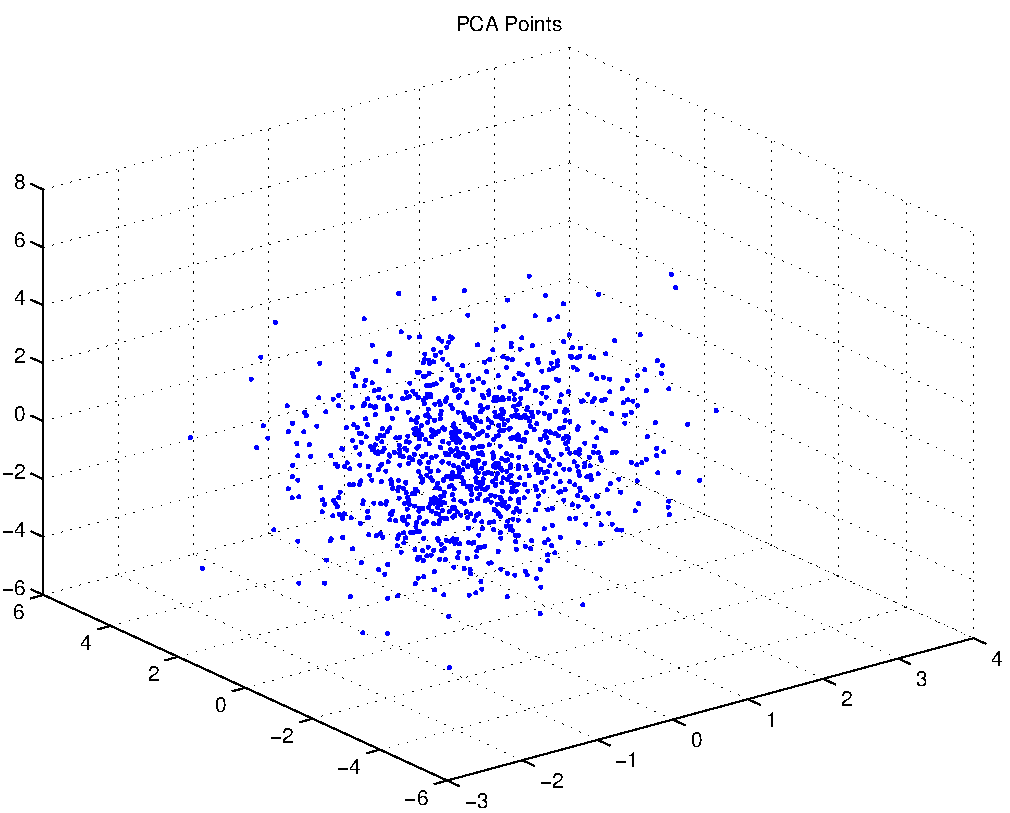
\includegraphics[width=10.0cm,height=10.0cm]{PCAPoints.pdf}

The eigenvectors:
+0.069, +0.174, +0.982
+0.222, +0.957, -0.185
-0.973, +0.231, +0.028

All of the eigenvalues of the covariance matrix:
(+0.958,+0.000), (+2.025,+0.000), (+3.017,+0.000)

QueryPerformanceCounter  =  +0.938
\subsubsection{Multi Variate Random Number Generator }
Sample from $N(\mu,\Sigma)$
mean= -0.002, variance=+1.004, skewness=+0.006, kurtosis=+3.003
mean= -0.001, variance=+1.017, skewness=-0.005, kurtosis=+2.988
mean= -0.002, variance=+1.006, skewness=-0.016, kurtosis=+3.014
Covariance Matrix 
+1.004, +0.009, +0.003
+0.009, +1.017, -0.003
+0.003, -0.003, +1.006

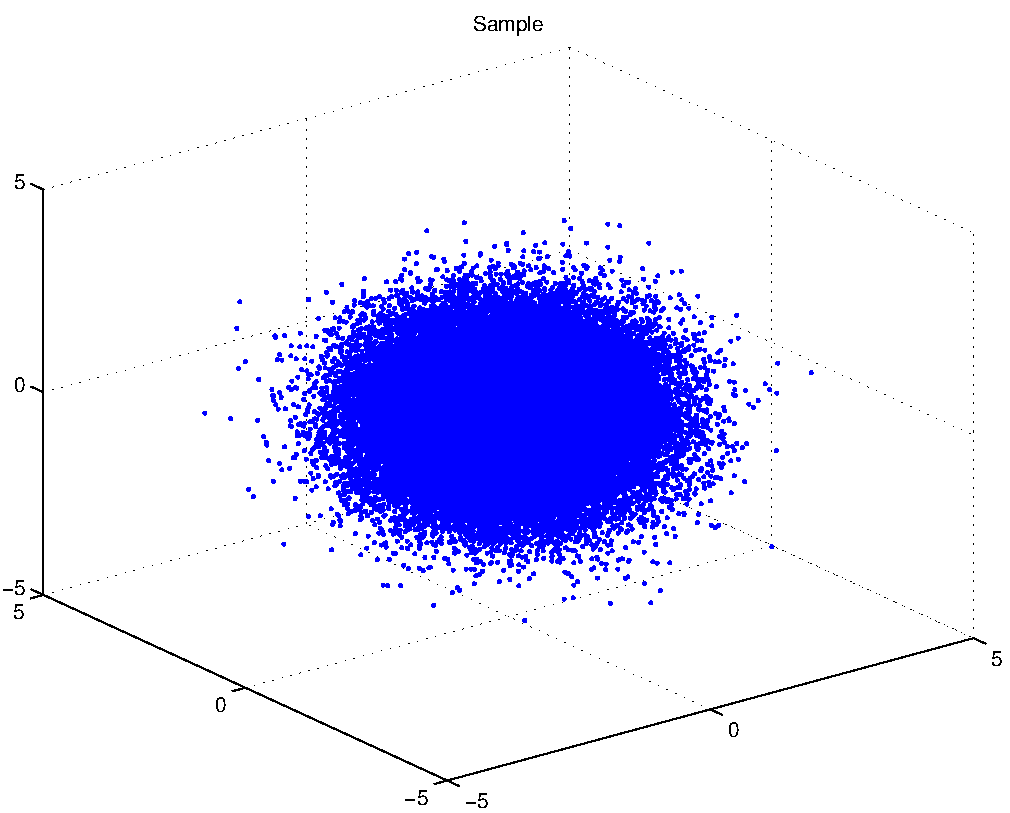
\includegraphics[width=10.0cm,height=10.0cm]{R_3_Normal.pdf}

Generate a sample from a unifom mixture of three Gaussians in $R^3$
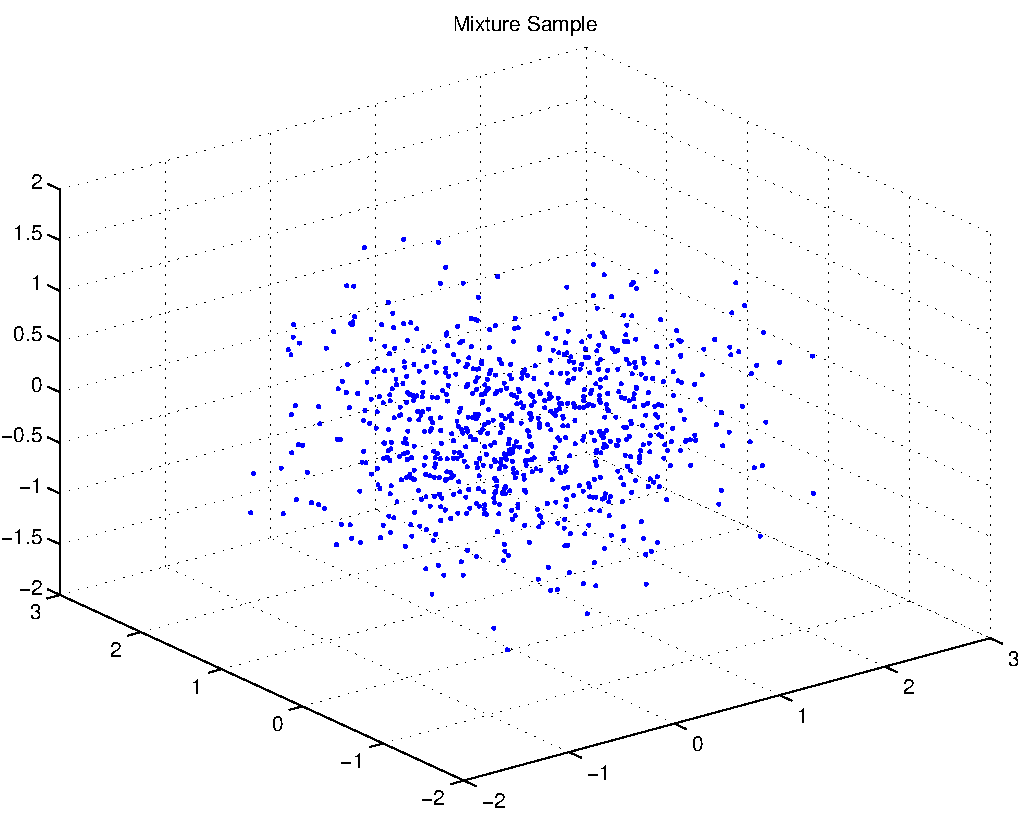
\includegraphics[width=10.0cm,height=10.0cm]{R_3_Normal_Mixture.pdf}

QueryPerformanceCounter  =  +13.774
\subsubsection{Matrix Multiply}
Comparing naive matrix multiply verus Intel MKL dgemm for matrix of size +2048.
This is for type double (hence the d in dgemm).
Naive type double matrix multiply tic toc  =  +0.440
dgemm plus row to column major transpose operation tic toc  =  +0.356
Comparing naive matrix multiply verus Intel MKL sgemm for matrix of size +2048.
This is for type float (hence the s in dgemm).
Naive type float matrix multiply tic toc  =  +0.271
sgemm plus row to column major transpose operation tic toc  =  +0.214
QueryPerformanceCounter  =  +1.414
\subsubsection{Descriptive Statistics}
Mean N(0,1): +0.003
Variance N(0,1): +1.006
Mean N(0,1) [recurrence relation method] :+0.003
Variance [recurrence relation method] :+1.006
Skewness : +0.007
Kurtosis : +2.997
QueryPerformanceCounter  =  +0.019
\subsubsection{Time Series }
+0.093
+0.726
+0.011
+2.178
QueryPerformanceCounter  =  +0.027
QueryPerformanceCounter  =  +6.327
\subsubsection{Iterated Exponential Filtering }
$\mu_1 =+0.093$
$\mu_2 =+0.726$
$\mu_3 =+0.011$
$\mu_4 =+2.178$
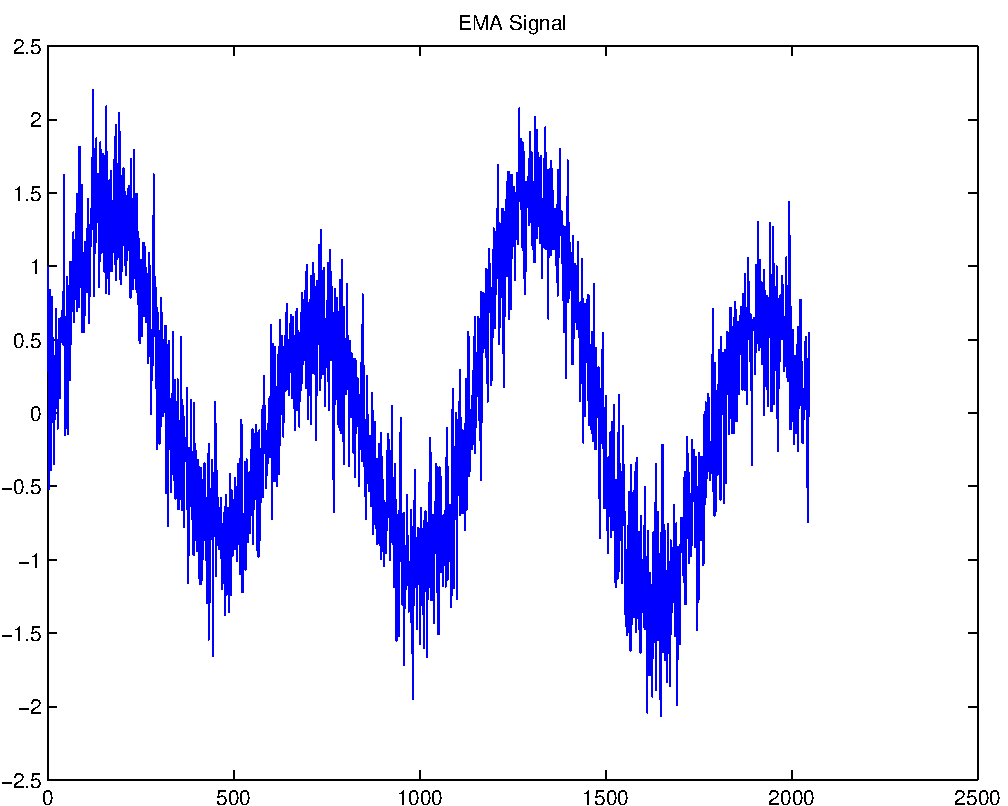
\includegraphics[width=10.0cm,height=10.0cm]{EMA_signal.pdf}

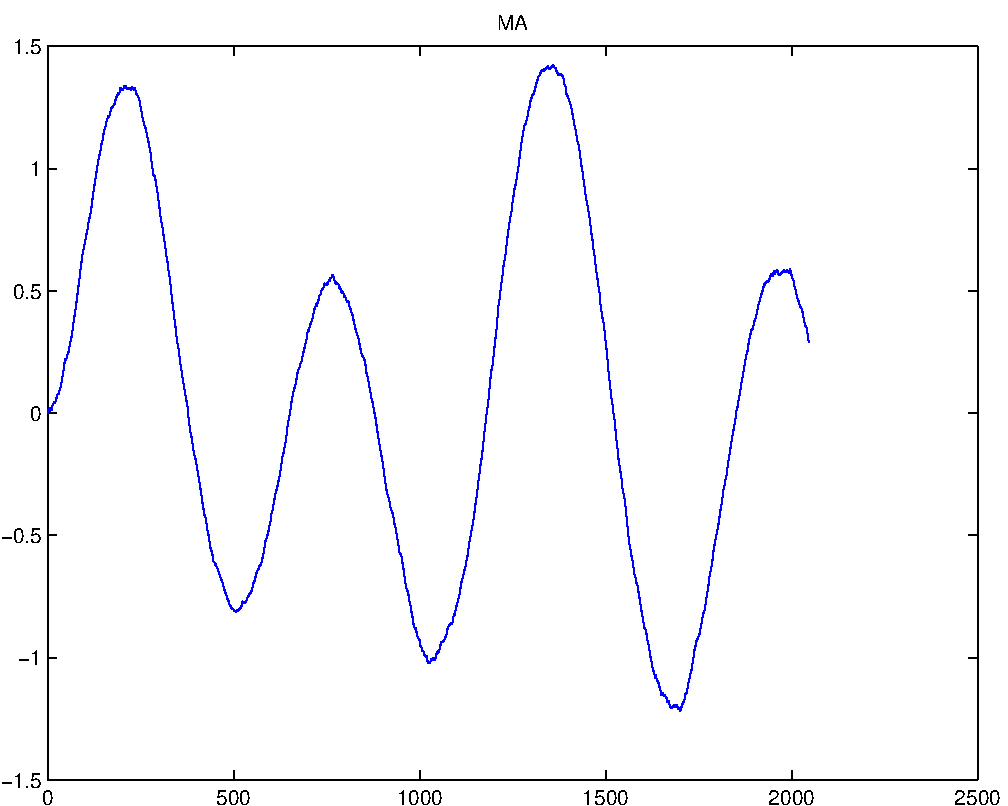
\includegraphics[width=10.0cm,height=10.0cm]{MA.pdf}

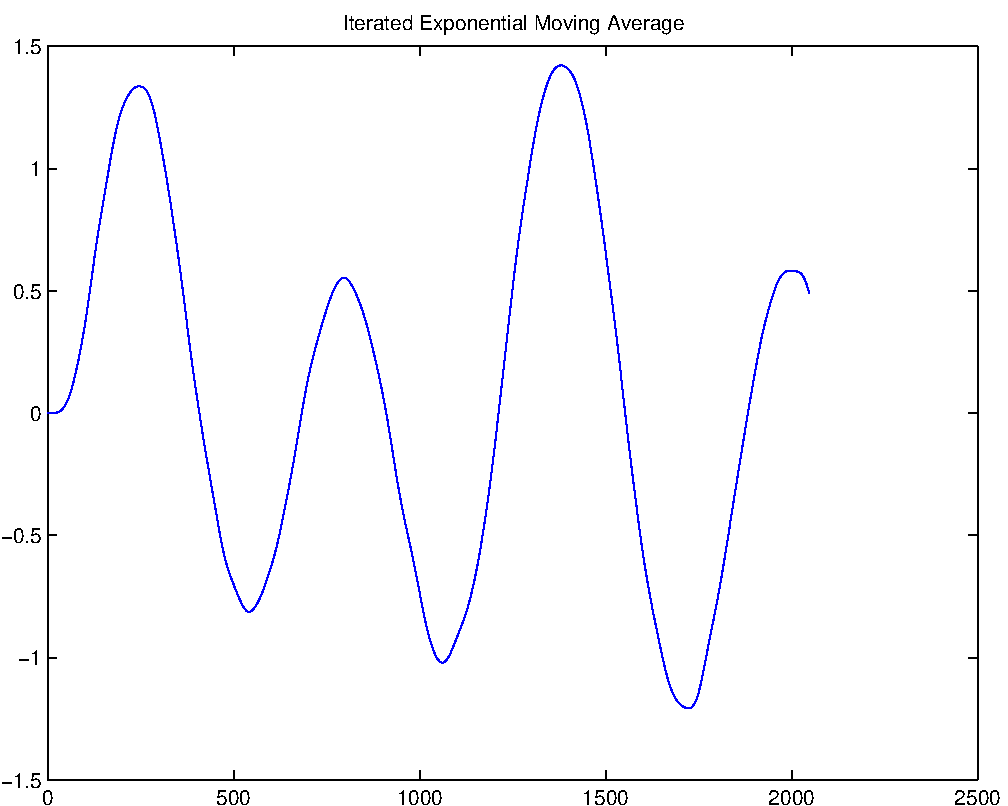
\includegraphics[width=10.0cm,height=10.0cm]{IEMA.pdf}

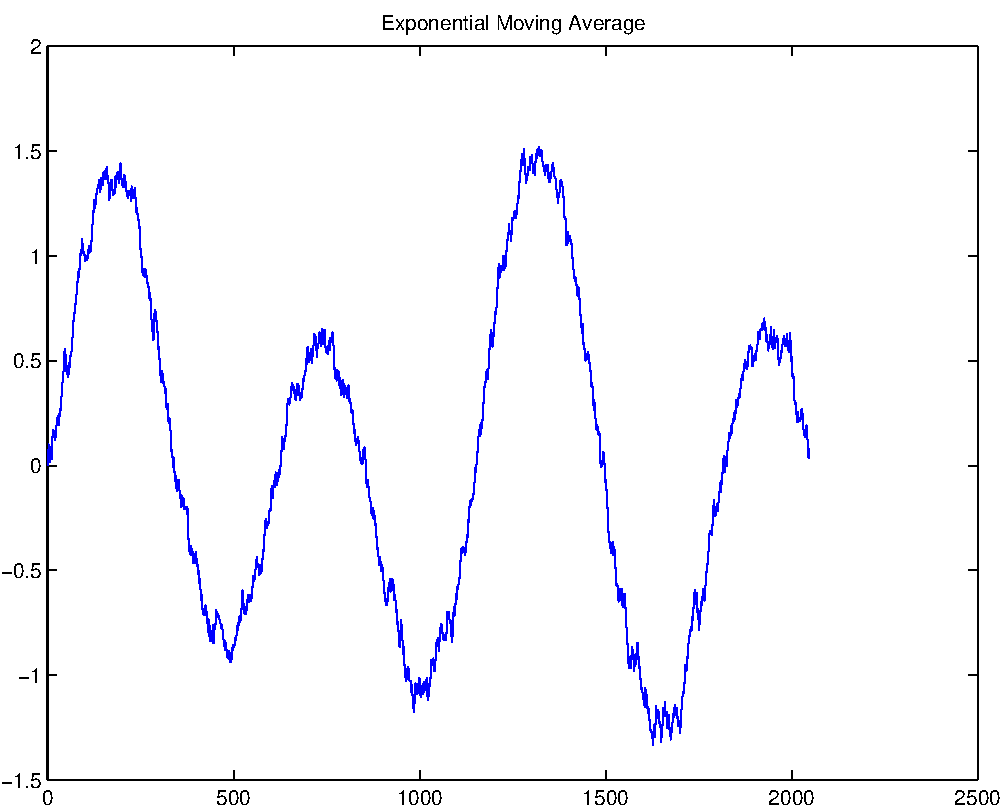
\includegraphics[width=10.0cm,height=10.0cm]{EMA.pdf}

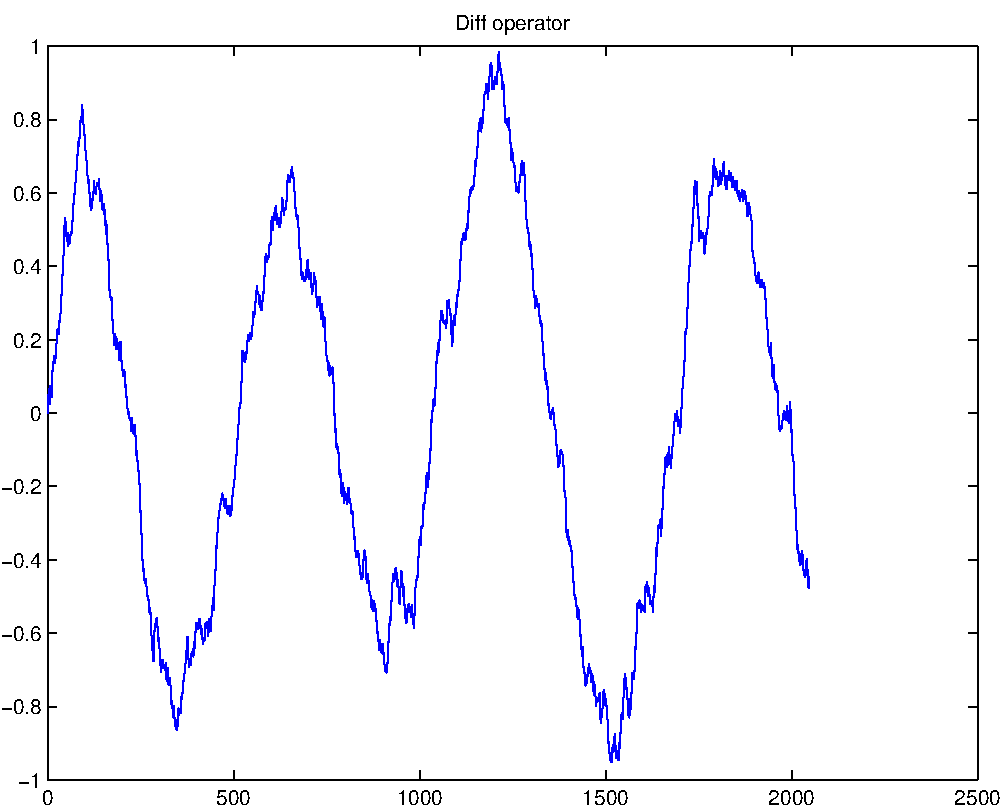
\includegraphics[width=10.0cm,height=10.0cm]{DIFF.pdf}

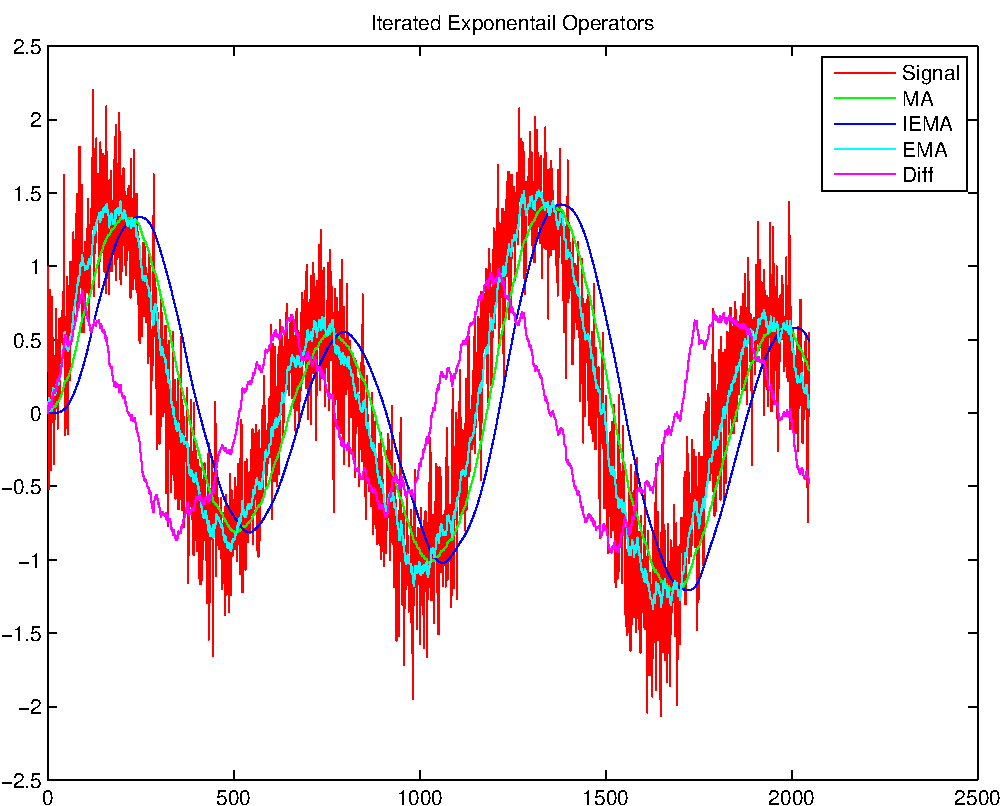
\includegraphics[width=10.0cm,height=10.0cm]{IteratedExponentailOperators.pdf}

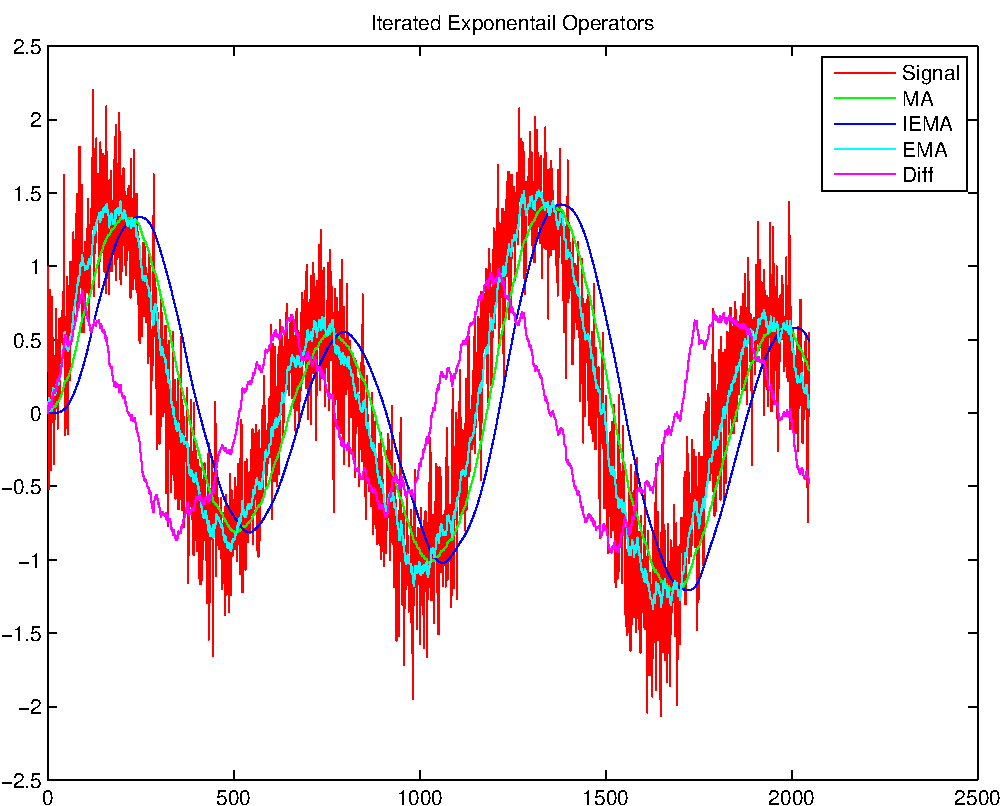
\includegraphics[width=10.0cm,height=10.0cm]{IteratedExponentailOperators.pdf}

QueryPerformanceCounter  =  +8.163
\subsubsection{Testing binary writer}
Binary writer Speedup 1GB Double Matrix +43.014

Binary reader Speedup 1GB Double Matrix +207.620

Binary writer Speedup 1GB Double vector +53.085

Binary reader Speedup 1GB Double Matrix +170.556

QueryPerformanceCounter  =  +0.890
\subsubsection{Testing Gaussian Mixture Point Cloud and Latex Plotting Capabilities.}
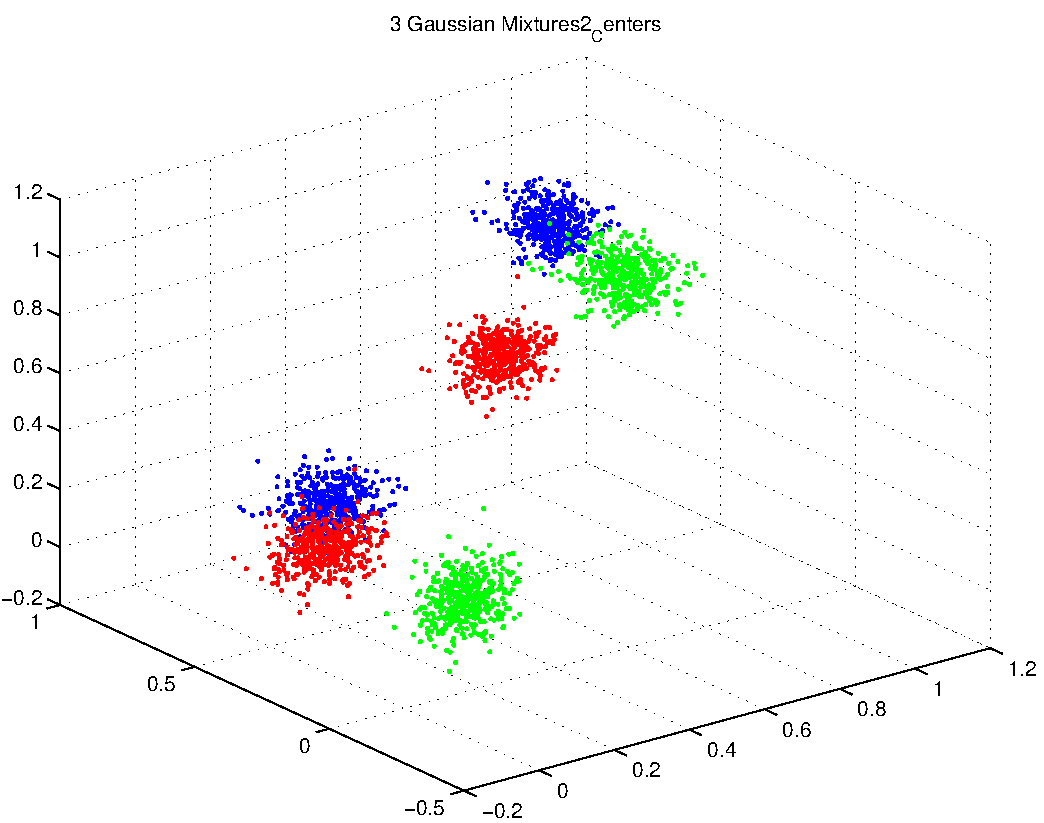
\includegraphics[width=10.0cm,height=10.0cm]{GaussianMixture_Dim_3_Centers2.pdf}

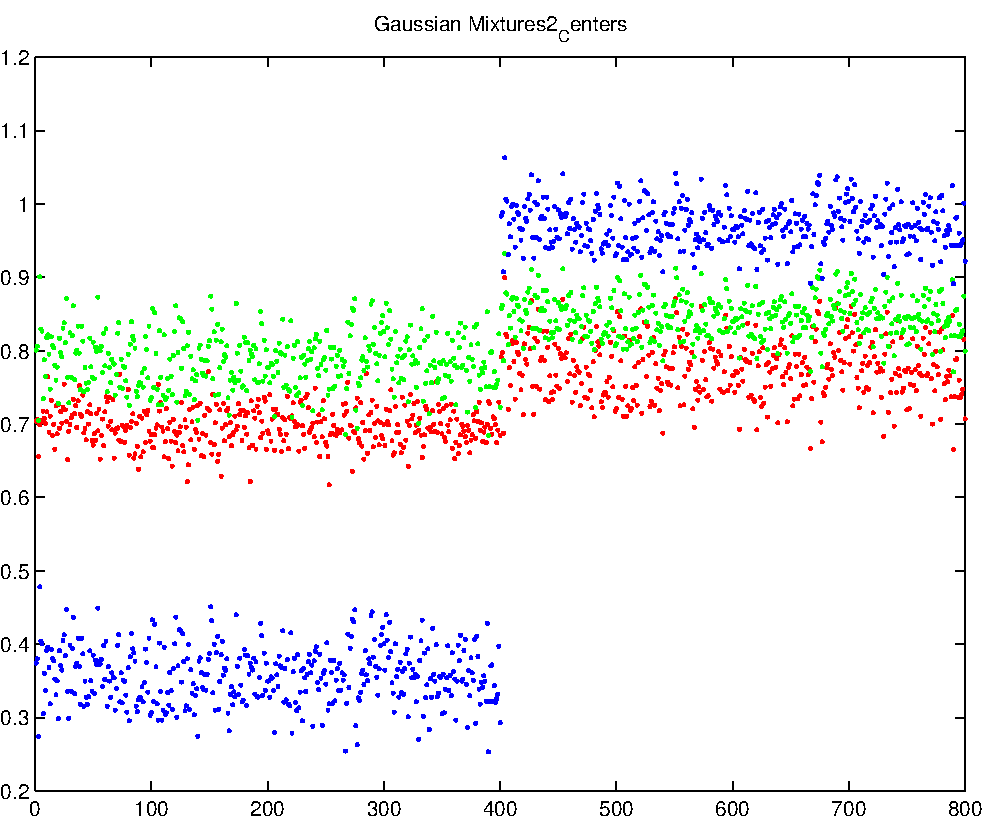
\includegraphics[width=10.0cm,height=10.0cm]{GaussianMixture_Dim_1_Centers2.pdf}

QueryPerformanceCounter  =  +2.785
\subsubsection{Intel VSL Function Check}
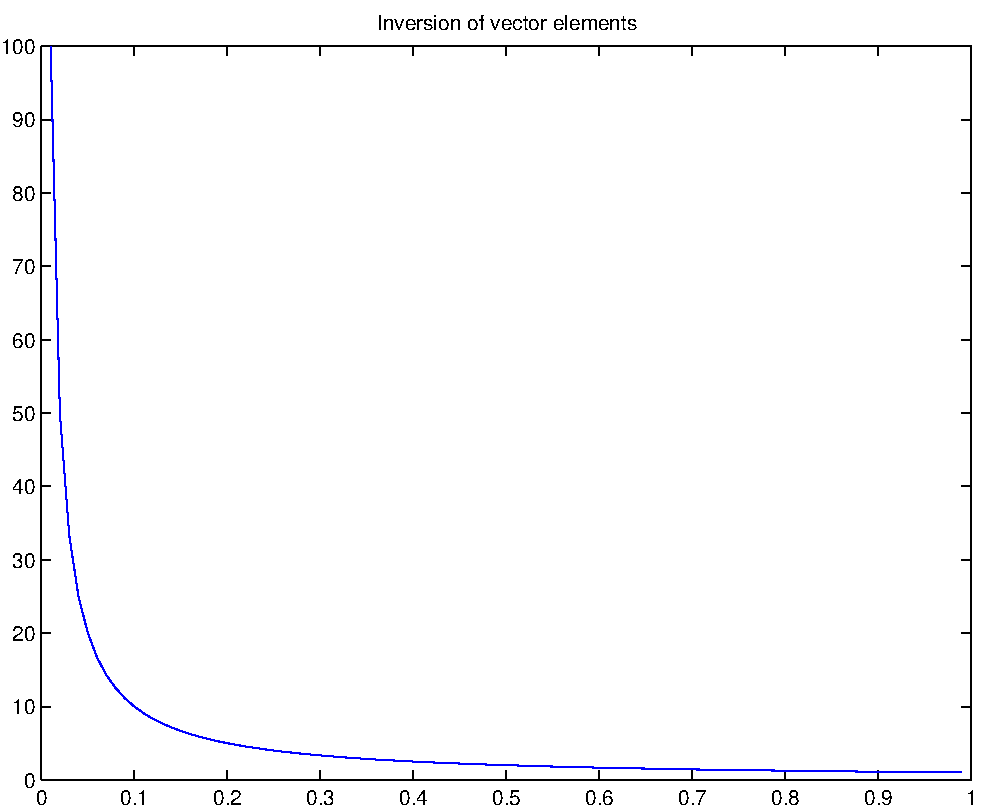
\includegraphics[width=10.0cm,height=10.0cm]{klVSLInv.pdf}

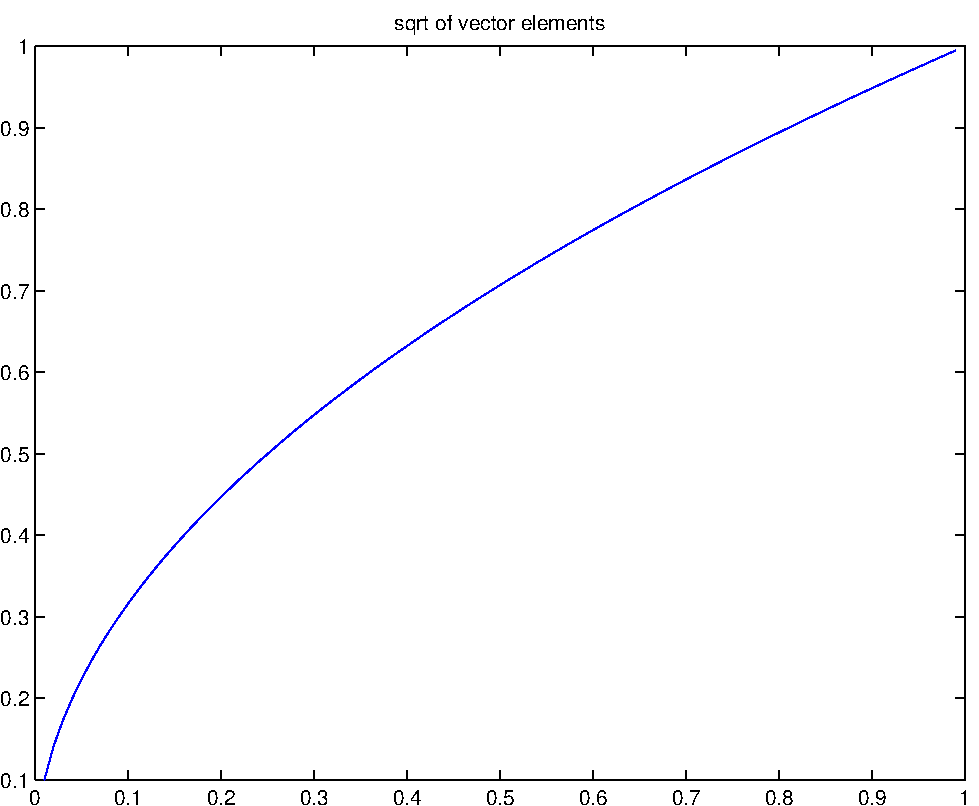
\includegraphics[width=10.0cm,height=10.0cm]{klVSLSqrt.pdf}

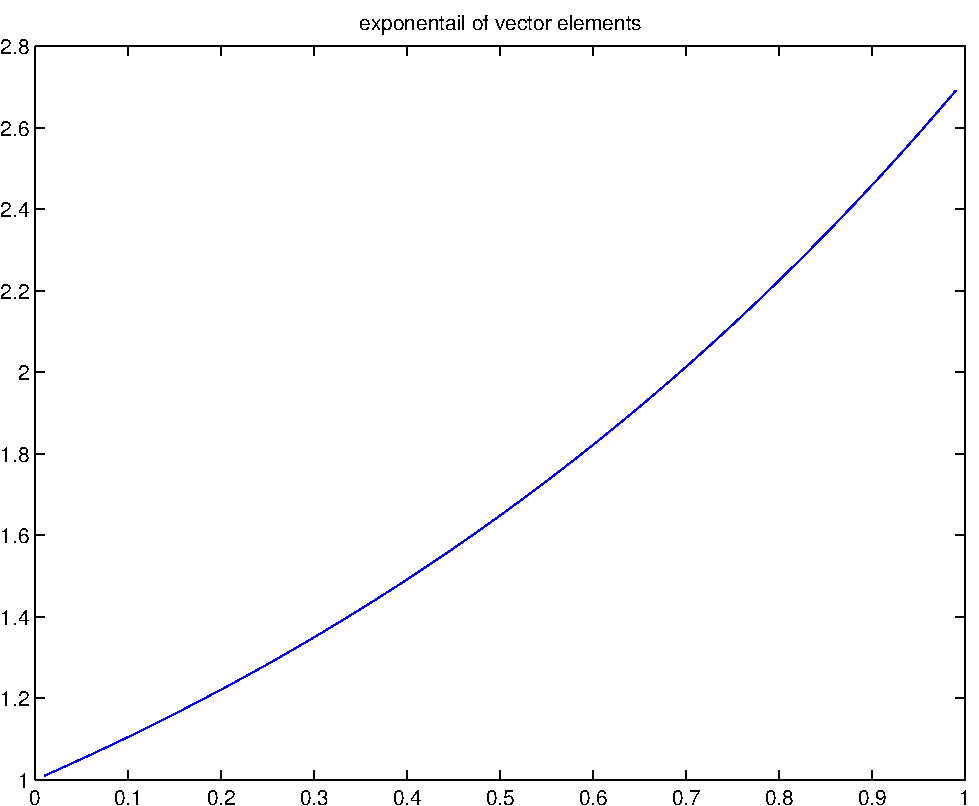
\includegraphics[width=10.0cm,height=10.0cm]{klVSLExp.pdf}

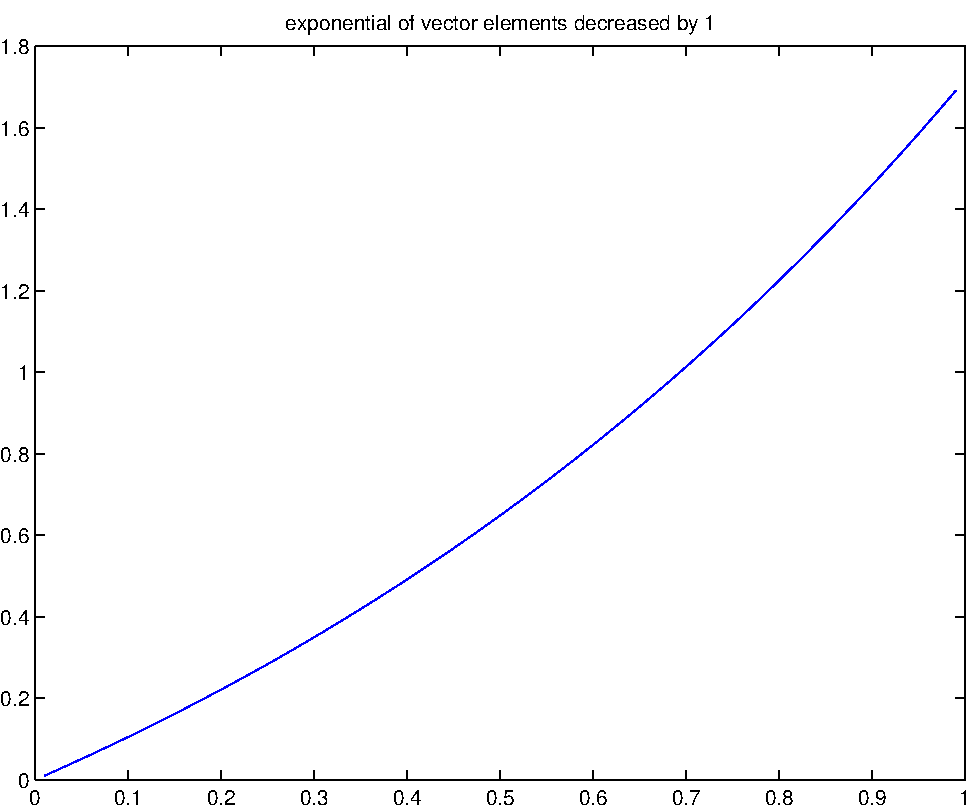
\includegraphics[width=10.0cm,height=10.0cm]{klVSLExpm1.pdf}

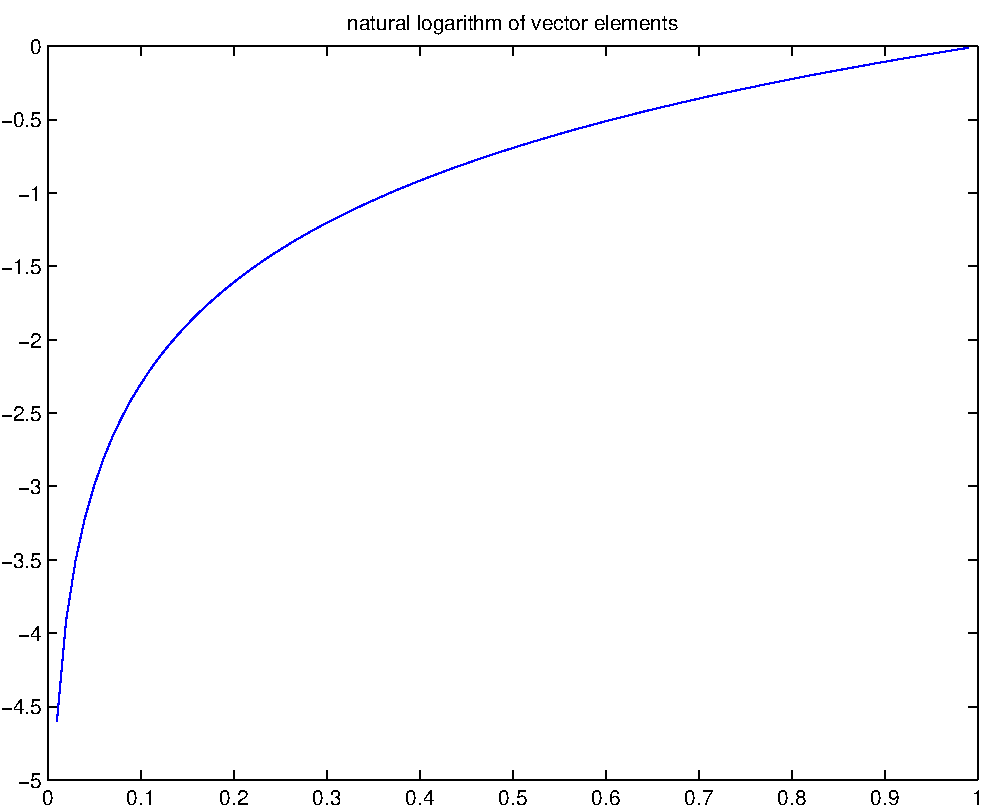
\includegraphics[width=10.0cm,height=10.0cm]{klVSLLn.pdf}

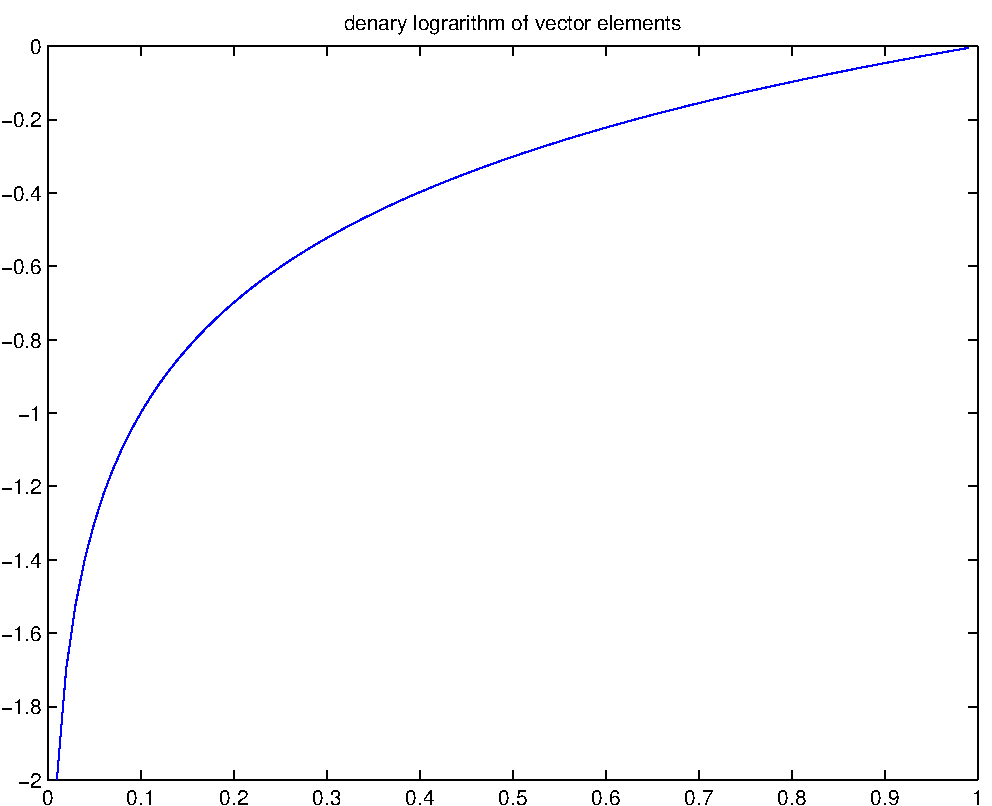
\includegraphics[width=10.0cm,height=10.0cm]{klVSLLog10.pdf}

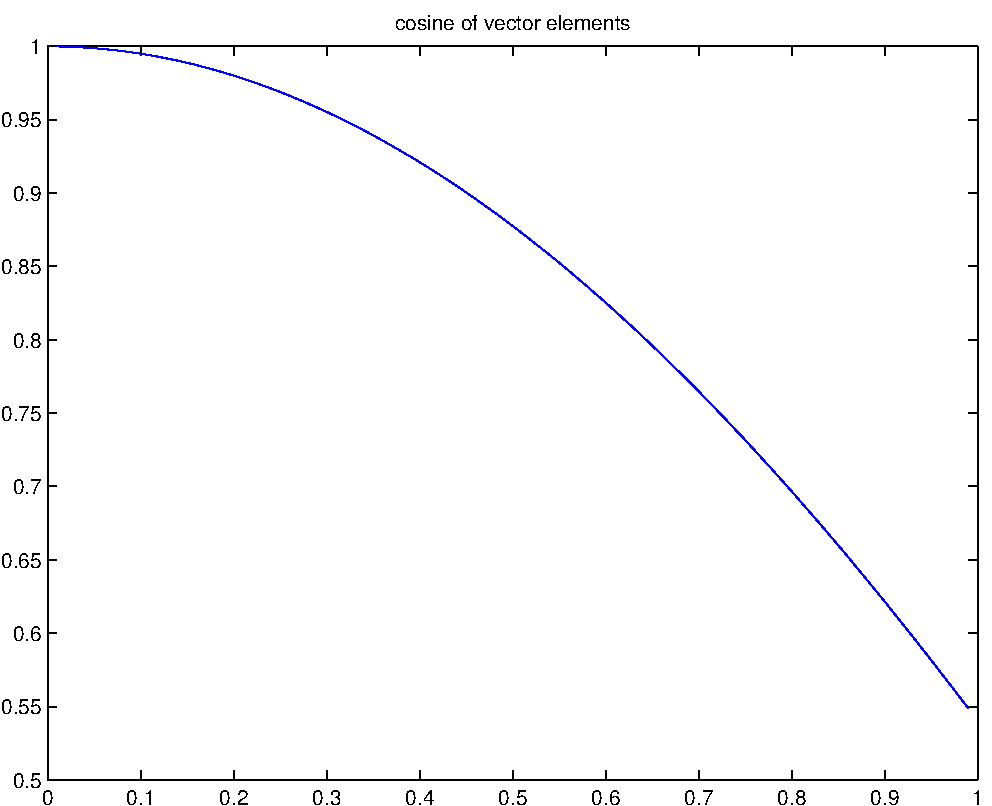
\includegraphics[width=10.0cm,height=10.0cm]{klVSLCos.pdf}

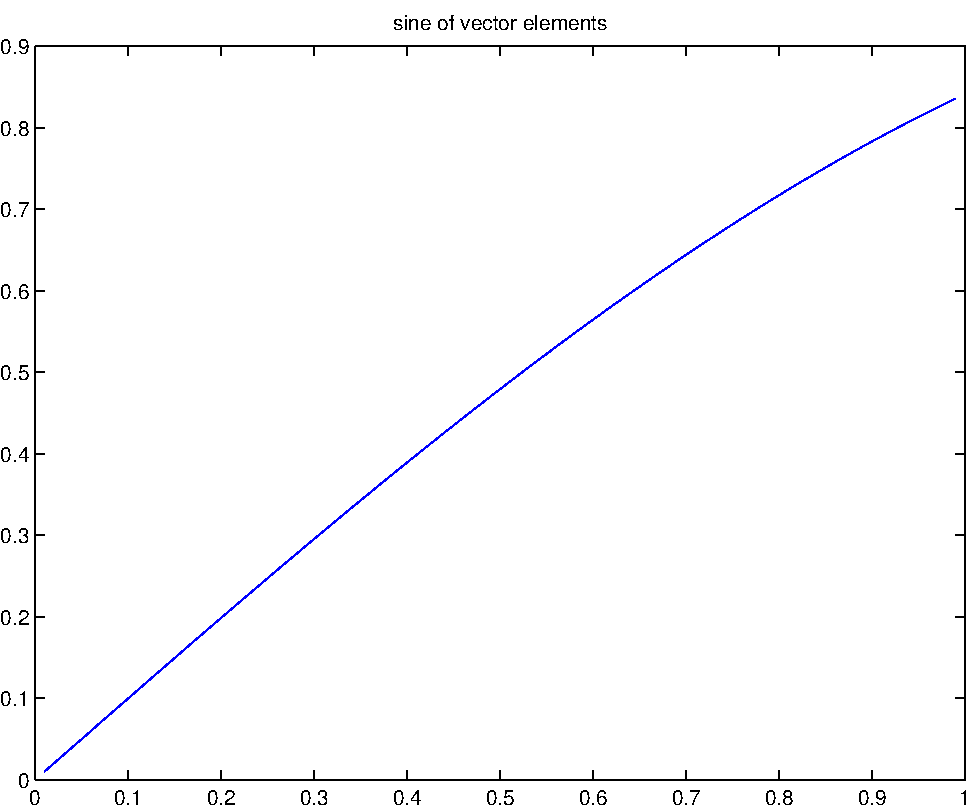
\includegraphics[width=10.0cm,height=10.0cm]{klVSLSin.pdf}

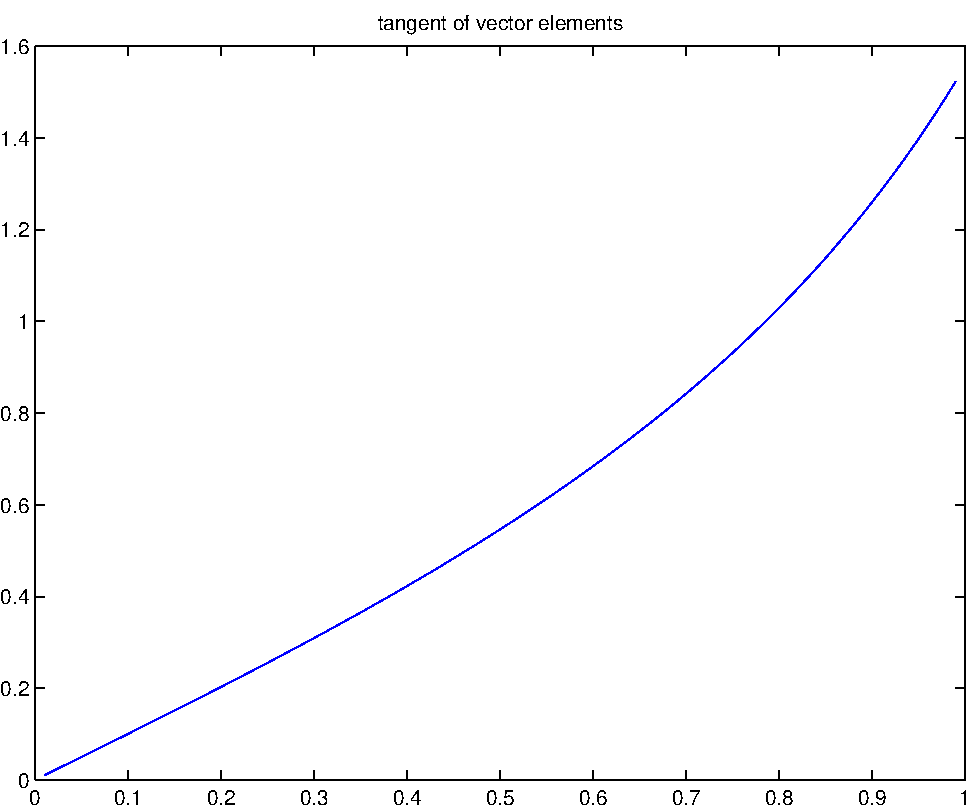
\includegraphics[width=10.0cm,height=10.0cm]{klVSLTan.pdf}

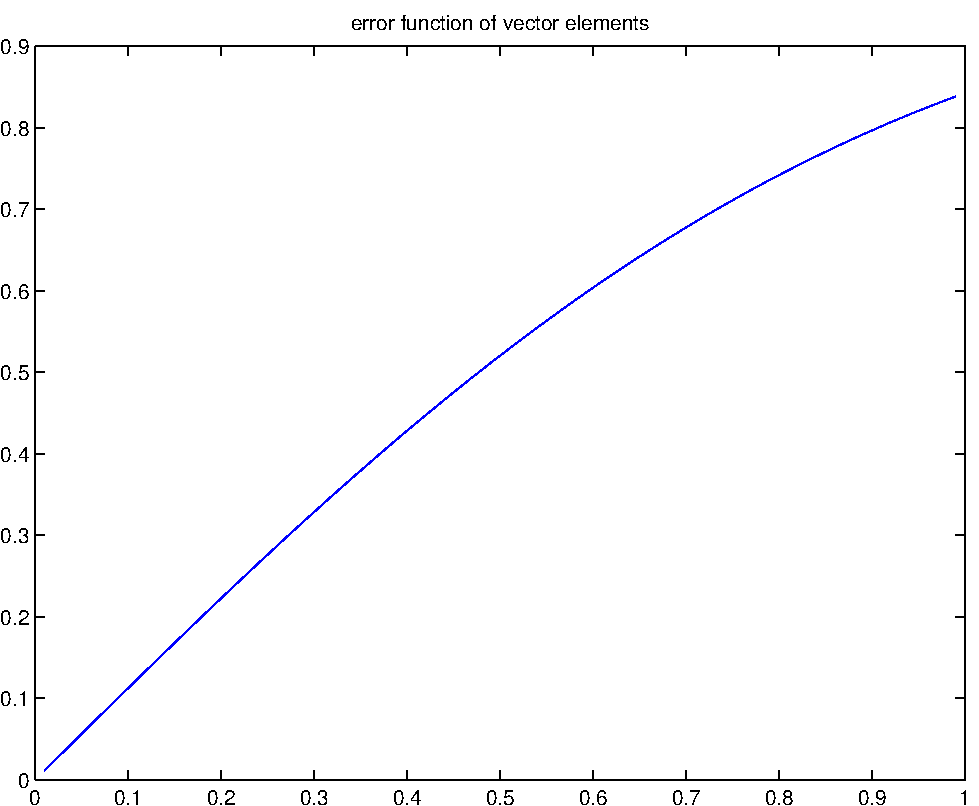
\includegraphics[width=10.0cm,height=10.0cm]{klVSLErf.pdf}

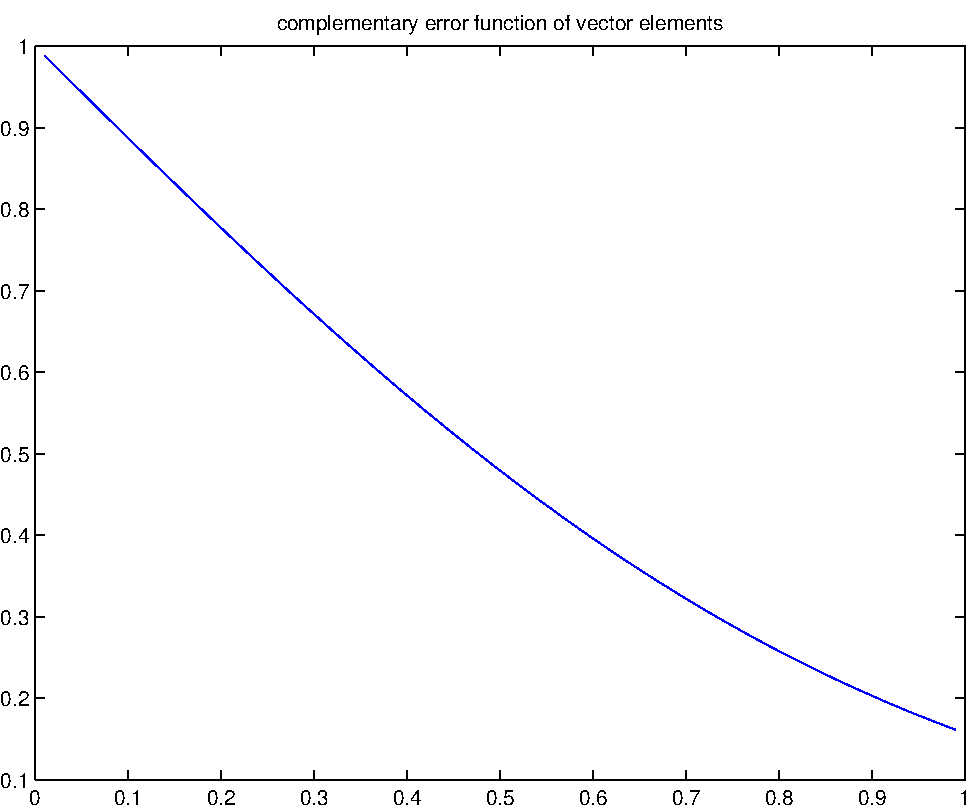
\includegraphics[width=10.0cm,height=10.0cm]{klVSLErfc.pdf}

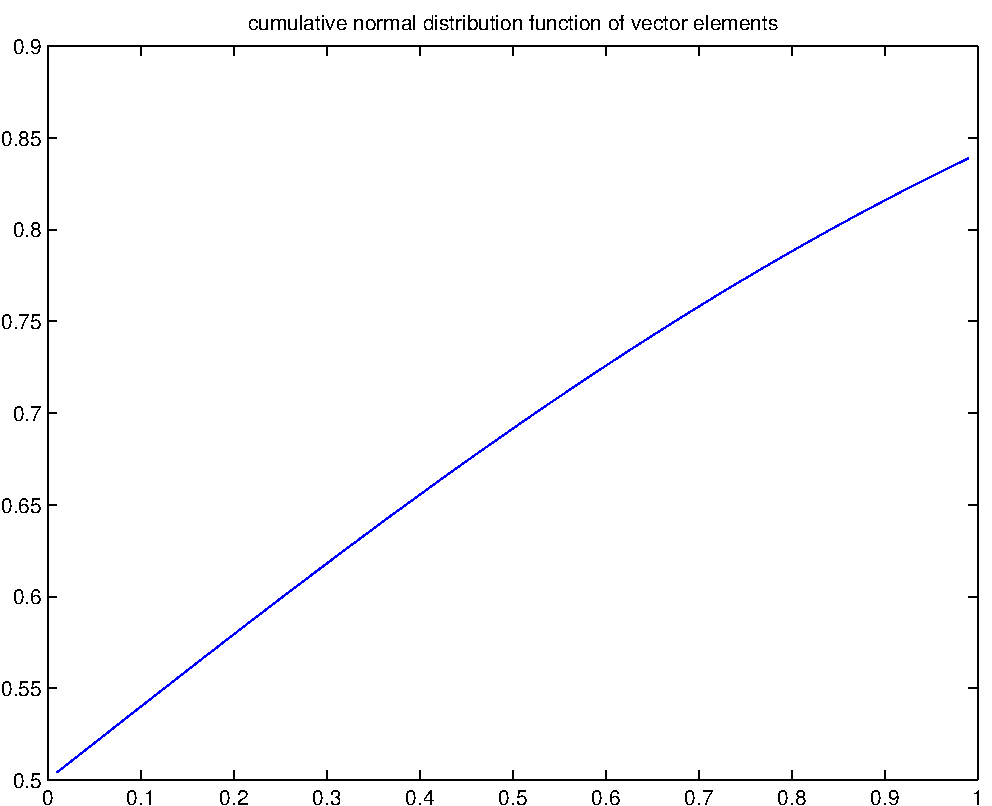
\includegraphics[width=10.0cm,height=10.0cm]{klVSLCdfNorm.pdf}

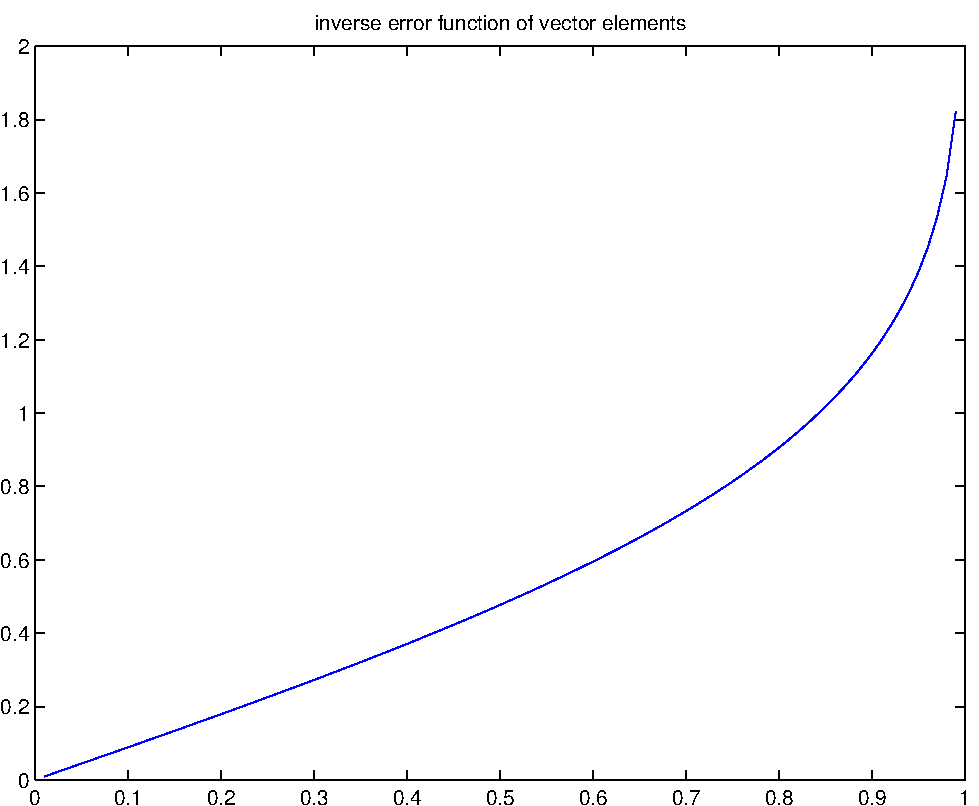
\includegraphics[width=10.0cm,height=10.0cm]{klVSLErfInv.pdf}

\includegraphics[width=10.0cm,height=10.0cm]{klVSLLGamma.pdf}

\includegraphics[width=10.0cm,height=10.0cm]{klVSLTGamma.pdf}

QueryPerformanceCounter  =  +15.299
\subsubsection{Gram Matrix Consistency Check}
Sample Size = 4096
Feature dim = 3

$$Sigma$ = \left(
\begin{array}{
ccc}
+1.140 & +1.535 & +0.581 \\
+1.535 & +9.988 & +1.605 \\
+0.581 & +1.605 & +0.428 \\
\end{array}
\right)$ \newline 

$Sample Covariance = \left(
\begin{array}{
ccc}
+1.132 & +1.589 & +0.588 \\
+1.589 & +10.005 & +1.650 \\
+0.588 & +1.650 & +0.438 \\
\end{array}
\right)$ \newline 

$Sample Mean = \left(
\begin{array}{
ccc}
+0.98501 & +1.03346 & +0.99391 \\
\end{array}
\right)$ \newline 

$Sample Covariance-$Omega$ = \left(
\begin{array}{
ccc}
-0.008 & +0.054 & +0.006 \\
+0.054 & +0.016 & +0.045 \\
+0.006 & +0.045 & +0.011 \\
\end{array}
\right)$ \newline 

$Sample Covariance Eigs = \left(
\begin{array}{
ccc}
(+10.57486,+0.00000) & (+0.96056,+0.00000) & (+0.03944,+0.00000) \\
\end{array}
\right)$ \newline 

$Centered Mean = \left(
\begin{array}{
ccc}
-0.00000 & -0.00000 & -0.00000 \\
\end{array}
\right)$ \newline 

$Centered Covariance = \left(
\begin{array}{
ccc}
+1.132 & +1.589 & +0.588 \\
+1.589 & +10.005 & +1.650 \\
+0.588 & +1.650 & +0.438 \\
\end{array}
\right)$ \newline 

$Gram Matrix Gf Not scaled by sample size = \left(
\begin{array}{
ccc}
+4636.570 & +6507.340 & +2407.206 \\
+6507.340 & +40978.762 & +6756.938 \\
+2407.206 & +6756.938 & +1795.327 \\
\end{array}
\right)$ \newline 

$Gram Matrix Gf  scaled by sample size = \left(
\begin{array}{
ccc}
+1.132 & +1.589 & +0.588 \\
+1.589 & +10.005 & +1.650 \\
+0.588 & +1.650 & +0.438 \\
\end{array}
\right)$ \newline 

$SampleCovariance - Scaled Gf = \left(
\begin{array}{
ccc}
+0.000 & +0.000 & +0.000 \\
+0.000 & +0.002 & +0.000 \\
+0.000 & +0.000 & +0.000 \\
\end{array}
\right)$ \newline 

$EigenDecomp of SampleCovariance = \left(
\begin{array}{
ccc}
-0.174 & -0.970 & -0.168 \\
+0.917 & -0.222 & +0.332 \\
-0.359 & -0.096 & +0.928 \\
\end{array}
\right)$ \newline 

$EigenDecomp of Gram Matrix = \left(
\begin{array}{
ccc}
-0.124 & -0.973 & -0.193 \\
-0.336 & +0.224 & -0.915 \\
+0.933 & -0.049 & -0.355 \\
\end{array}
\right)$ \newline 

QueryPerformanceCounter  =  +1.366
\subsubsection{Eigen Solver Checks}
\subsubsection{Haar Distributed Random Orthogonal Matrix $A \in O(n)$}
 Testing Operator Norm
Number of Dimensions: +8

$A = \left(
\begin{array}{
cccccccc}
+0.258 & -0.111 & -0.044 & +0.468 & +0.192 & +0.268 & +0.078 & -0.765 \\
+0.183 & -0.392 & +0.464 & -0.311 & -0.483 & -0.063 & +0.475 & -0.193 \\
-0.179 & +0.648 & +0.275 & -0.319 & -0.267 & +0.383 & -0.224 & -0.321 \\
-0.739 & -0.227 & -0.395 & +0.138 & -0.354 & +0.227 & +0.204 & -0.098 \\
+0.302 & -0.348 & -0.502 & -0.509 & -0.157 & +0.163 & -0.447 & -0.158 \\
-0.165 & -0.339 & +0.307 & -0.212 & +0.511 & +0.644 & +0.032 & +0.204 \\
-0.285 & +0.080 & -0.131 & -0.495 & +0.498 & -0.414 & +0.271 & -0.397 \\
+0.350 & +0.347 & -0.433 & -0.119 & +0.009 & +0.336 & +0.634 & +0.204 \\
\end{array}
\right)$ \newline 

$Det(A) :   A \in O(n)$ = (+1.000,+0.000)

$L = \left(
\begin{array}{
cccccccc}
+1.000 & +0.000 & +0.000 & +0.000 & +0.000 & +0.000 & +0.000 & +0.000 \\
+0.243 & +1.000 & +0.000 & +0.000 & +0.000 & +0.000 & +0.000 & +0.000 \\
-0.473 & +0.341 & +1.000 & +0.000 & +0.000 & +0.000 & +0.000 & +0.000 \\
-0.410 & -0.627 & +0.578 & +1.000 & +0.000 & +0.000 & +0.000 & +0.000 \\
+0.386 & +0.239 & +0.090 & +0.660 & +1.000 & +0.000 & +0.000 & +0.000 \\
+0.223 & -0.410 & -0.734 & +0.475 & +0.666 & +1.000 & +0.000 & +0.000 \\
-0.248 & -0.638 & -0.809 & +0.628 & -0.582 & -0.116 & +1.000 & +0.000 \\
-0.350 & -0.272 & +0.109 & -0.581 & -0.195 & +0.296 & -0.252 & +1.000 \\
\end{array}
\right)$ \newline 

$U = \left(
\begin{array}{
cccccccc}
-0.739 & -0.227 & -0.395 & +0.138 & -0.354 & +0.227 & +0.204 & -0.098 \\
+0.000 & +0.703 & +0.371 & -0.352 & -0.181 & +0.328 & -0.273 & -0.297 \\
+0.000 & +0.000 & -0.746 & +0.067 & -0.096 & +0.331 & +0.824 & +0.259 \\
+0.000 & +0.000 & +0.000 & -0.712 & -0.360 & +0.270 & -1.011 & -0.535 \\
+0.000 & +0.000 & +0.000 & +0.000 & +0.924 & -0.788 & +0.851 & +0.042 \\
+0.000 & +0.000 & +0.000 & +0.000 & +0.000 & +1.368 & +0.393 & +0.520 \\
+0.000 & +0.000 & +0.000 & +0.000 & +0.000 & +0.000 & +2.194 & +0.224 \\
+0.000 & +0.000 & +0.000 & +0.000 & +0.000 & +0.000 & +0.000 & -1.308 \\
\end{array}
\right)$ \newline 

$L * U  = \left(
\begin{array}{
cccccccc}
-0.739 & -0.227 & -0.395 & +0.138 & -0.354 & +0.227 & +0.204 & -0.098 \\
-0.179 & +0.648 & +0.275 & -0.319 & -0.267 & +0.383 & -0.224 & -0.321 \\
+0.350 & +0.347 & -0.433 & -0.119 & +0.009 & +0.336 & +0.634 & +0.204 \\
+0.302 & -0.348 & -0.502 & -0.509 & -0.157 & +0.163 & -0.447 & -0.158 \\
-0.285 & +0.080 & -0.131 & -0.495 & +0.498 & -0.414 & +0.271 & -0.397 \\
-0.165 & -0.339 & +0.307 & -0.212 & +0.511 & +0.644 & +0.032 & +0.204 \\
+0.183 & -0.392 & +0.464 & -0.311 & -0.483 & -0.063 & +0.475 & -0.193 \\
+0.258 & -0.111 & -0.044 & +0.468 & +0.192 & +0.268 & +0.078 & -0.765 \\
\end{array}
\right)$ \newline 

$Det(L) :    = (+1.000,+0.000)     Det(U) :    = (+1.000,+0.000)     Det(LU) :    = (+1.000,+0.000)$

$||A||_{L_1}$  = +2.571

$||A||_{L_{\infty}}$ = +2.616

$||A^{-1}||_{L_1}$  = +2.616

$||A^{-1}||_{L_{\infty}}$ = +2.571

$||A||_{L_{\infty}} * ||A^{-1}||_{L_{\infty}} = +6.724$

$||A||_{L_1} * ||A^{-1}||_{L_1} = +6.724$

Frobenious Norm  $||A||_{\textit{F}}$ via $\sum\limits_{i,j =0}^{n} \|A_{i,j}|$   of  $A \in O(n)$  +2.828

$L_1$ condition number of Haar Distributed Random Orthogonal Matrix $A \in O(n)$ +6.122

$A = \left(
\begin{array}{
cccccccc}
+0.258 & -0.111 & -0.044 & +0.468 & +0.192 & +0.268 & +0.078 & -0.765 \\
+0.183 & -0.392 & +0.464 & -0.311 & -0.483 & -0.063 & +0.475 & -0.193 \\
-0.179 & +0.648 & +0.275 & -0.319 & -0.267 & +0.383 & -0.224 & -0.321 \\
-0.739 & -0.227 & -0.395 & +0.138 & -0.354 & +0.227 & +0.204 & -0.098 \\
+0.302 & -0.348 & -0.502 & -0.509 & -0.157 & +0.163 & -0.447 & -0.158 \\
-0.165 & -0.339 & +0.307 & -0.212 & +0.511 & +0.644 & +0.032 & +0.204 \\
-0.285 & +0.080 & -0.131 & -0.495 & +0.498 & -0.414 & +0.271 & -0.397 \\
+0.350 & +0.347 & -0.433 & -0.119 & +0.009 & +0.336 & +0.634 & +0.204 \\
\end{array}
\right)$ \newline 

$L_{\infty}$ condition number of Haar Distributed Random Orthogonal Matrix $A \in O(n)$ +6.724

Eigenvalues of $A \in O(n)$

(-0.964,+0.266), (-0.964,-0.266), (-0.019,+1.000), (-0.019,-1.000), (+0.606,+0.795), (+0.606,-0.795), (+0.998,+0.070), (+0.998,-0.070)

 $|\lambda | : \lambda \in \sigma(A) , A \in O(n)$

+1.000, +1.000, +1.000, +1.000, +1.000, +1.000, +1.000, +1.000


Calculating $A^{\dag} A,$  we expect $A^{\dag} A \approx I$

$A^{\dag} A = \left(
\begin{array}{
cccccccc}
+1.000 & -0.000 & -0.000 & +0.000 & -0.000 & +0.000 & +0.000 & +0.000 \\
-0.000 & +1.000 & +0.000 & +0.000 & -0.000 & +0.000 & -0.000 & -0.000 \\
-0.000 & +0.000 & +1.000 & +0.000 & +0.000 & +0.000 & -0.000 & +0.000 \\
+0.000 & +0.000 & +0.000 & +1.000 & +0.000 & -0.000 & -0.000 & +0.000 \\
-0.000 & -0.000 & +0.000 & +0.000 & +1.000 & +0.000 & +0.000 & -0.000 \\
+0.000 & +0.000 & +0.000 & -0.000 & +0.000 & +1.000 & +0.000 & +0.000 \\
+0.000 & -0.000 & -0.000 & -0.000 & +0.000 & +0.000 & +1.000 & -0.000 \\
+0.000 & -0.000 & +0.000 & +0.000 & -0.000 & +0.000 & -0.000 & +1.000 \\
\end{array}
\right)$ \newline 

Calculating $A^{-1} ,  A \in O(n)$.

$A^{-1} = \left(
\begin{array}{
cccccccc}
+0.258 & +0.183 & -0.179 & -0.739 & +0.302 & -0.165 & -0.285 & +0.350 \\
-0.111 & -0.392 & +0.648 & -0.227 & -0.348 & -0.339 & +0.080 & +0.347 \\
-0.044 & +0.464 & +0.275 & -0.395 & -0.502 & +0.307 & -0.131 & -0.433 \\
+0.468 & -0.311 & -0.319 & +0.138 & -0.509 & -0.212 & -0.495 & -0.119 \\
+0.192 & -0.483 & -0.267 & -0.354 & -0.157 & +0.511 & +0.498 & +0.009 \\
+0.268 & -0.063 & +0.383 & +0.227 & +0.163 & +0.644 & -0.414 & +0.336 \\
+0.078 & +0.475 & -0.224 & +0.204 & -0.447 & +0.032 & +0.271 & +0.634 \\
-0.765 & -0.193 & -0.321 & -0.098 & -0.158 & +0.204 & -0.397 & +0.204 \\
\end{array}
\right)$ \newline 

Calculating $A^{-1} *A  ,  A \in O(n)$.   We expect $A^{-1} *A  \approx I$. 

$A^{-1} *A = \left(
\begin{array}{
cccccccc}
+1.000 & -0.000 & -0.000 & -0.000 & +0.000 & -0.000 & +0.000 & +0.000 \\
-0.000 & +1.000 & +0.000 & +0.000 & -0.000 & -0.000 & +0.000 & -0.000 \\
+0.000 & +0.000 & +1.000 & +0.000 & +0.000 & +0.000 & -0.000 & +0.000 \\
-0.000 & -0.000 & -0.000 & +1.000 & +0.000 & -0.000 & -0.000 & +0.000 \\
-0.000 & -0.000 & +0.000 & +0.000 & +1.000 & +0.000 & +0.000 & +0.000 \\
+0.000 & +0.000 & +0.000 & -0.000 & +0.000 & +1.000 & +0.000 & +0.000 \\
+0.000 & +0.000 & +0.000 & +0.000 & +0.000 & +0.000 & +1.000 & +0.000 \\
+0.000 & -0.000 & +0.000 & -0.000 & +0.000 & +0.000 & +0.000 & +1.000 \\
\end{array}
\right)$ \newline 

Calculating SVD of  $A \in O(n)$

$U = \left(
\begin{array}{
cccccccc}
-0.005 & -0.150 & +0.568 & -0.139 & +0.664 & +0.125 & -0.416 & +0.071 \\
+0.571 & +0.718 & +0.147 & +0.036 & -0.168 & +0.124 & -0.295 & +0.073 \\
-0.088 & -0.022 & +0.271 & -0.619 & -0.377 & -0.154 & -0.161 & -0.586 \\
+0.664 & -0.649 & -0.064 & -0.056 & -0.226 & -0.091 & -0.199 & +0.179 \\
-0.258 & +0.111 & +0.044 & -0.468 & -0.192 & -0.268 & -0.078 & +0.765 \\
-0.112 & +0.067 & -0.154 & +0.342 & +0.072 & -0.766 & -0.484 & -0.130 \\
+0.369 & +0.122 & +0.147 & -0.198 & +0.358 & -0.515 & +0.626 & -0.050 \\
-0.103 & -0.093 & +0.729 & +0.467 & -0.409 & -0.115 & +0.203 & +0.101 \\
\end{array}
\right)$ \newline 

$S = \left(
\begin{array}{
cccccccc}
+1.000 & +0.000 & +0.000 & +0.000 & +0.000 & +0.000 & +0.000 & +0.000 \\
+0.000 & +1.000 & +0.000 & +0.000 & +0.000 & +0.000 & +0.000 & +0.000 \\
+0.000 & +0.000 & +1.000 & +0.000 & +0.000 & +0.000 & +0.000 & +0.000 \\
+0.000 & +0.000 & +0.000 & +1.000 & +0.000 & +0.000 & +0.000 & +0.000 \\
+0.000 & +0.000 & +0.000 & +0.000 & +1.000 & +0.000 & +0.000 & +0.000 \\
+0.000 & +0.000 & +0.000 & +0.000 & +0.000 & +1.000 & +0.000 & +0.000 \\
+0.000 & +0.000 & +0.000 & +0.000 & +0.000 & +0.000 & +1.000 & +0.000 \\
+0.000 & +0.000 & +0.000 & +0.000 & +0.000 & +0.000 & +0.000 & +1.000 \\
\end{array}
\right)$ \newline 

$V = \left(
\begin{array}{
cccccccc}
+0.000 & +0.000 & -0.000 & +0.000 & -1.000 & -0.000 & +0.000 & +0.000 \\
-0.175 & -0.202 & +0.539 & +0.350 & -0.000 & -0.416 & +0.316 & +0.493 \\
+0.045 & +0.526 & +0.539 & -0.526 & -0.000 & -0.251 & -0.301 & -0.003 \\
-0.504 & -0.617 & -0.000 & -0.324 & -0.000 & -0.110 & -0.496 & +0.024 \\
-0.072 & -0.002 & +0.359 & +0.568 & +0.000 & -0.052 & -0.316 & -0.664 \\
+0.677 & -0.300 & -0.180 & -0.041 & +0.000 & -0.622 & -0.154 & -0.083 \\
+0.122 & -0.386 & +0.359 & -0.405 & +0.000 & +0.161 & +0.564 & -0.446 \\
-0.484 & +0.249 & -0.359 & -0.082 & +0.000 & -0.580 & +0.348 & -0.332 \\
\end{array}
\right)$ \newline 

$U S V = \left(
\begin{array}{
cccccccc}
+0.074 & +0.555 & +0.266 & +0.229 & +0.005 & -0.286 & -0.589 & -0.368 \\
-0.113 & +0.006 & +0.251 & +0.175 & -0.571 & -0.498 & +0.058 & +0.563 \\
+0.515 & +0.493 & +0.179 & -0.044 & +0.088 & +0.439 & +0.066 & +0.503 \\
-0.017 & +0.281 & -0.585 & -0.234 & -0.664 & +0.225 & -0.123 & -0.135 \\
-0.329 & +0.591 & -0.240 & +0.039 & +0.258 & -0.284 & +0.579 & -0.026 \\
-0.711 & +0.079 & -0.011 & +0.272 & +0.112 & +0.443 & -0.325 & +0.316 \\
-0.189 & +0.074 & +0.609 & +0.005 & -0.369 & +0.366 & +0.395 & -0.403 \\
-0.258 & +0.096 & +0.253 & -0.886 & +0.103 & -0.128 & -0.184 & +0.121 \\
\end{array}
\right)$ \newline 

Calculating first few eigenvectors of $A \in O(n)$ using LAPACK syevx

\subsubsection{Wishart Matrix $A \in W(n)$}
$L_1$ condition number of Wishart Matrix +1489.694
$L_infty$ condition number of Wishart Matrix +1489.694
\subsubsection{Gaussian Orthogonal Ensemble $A \in GOE(n)$}
$L_1$ condition number of GOE Matrix +66.900
$L_\infty$ condition number of GOE Matrix +66.900
\subsubsection{The Identity Matrix $I \in M(n)$}
$L_1$ condition number of $I$ = +1.000
$L_\infty$ condition number of $I$ = +1.000
QueryPerformanceCounter  =  +0.331
\subsubsection{Generate Tracey Widom Sample}
\subsubsection{Sample from $W_n m$ times and calculate empirical PDF of the first eig}
Here we generate histograms of $\lambda_1$ for GOE (Gaussian Orthogonal Ensemble), and W (Wishart) 		 distributed of random matrices
These should approximate the celebrated Tracy Widom distribution.
Dimension $n = +1024$

Sample size $m = 1024$

\includegraphics[width=10.0cm,height=10.0cm]{Re_TraceyWidom.pdf}

\includegraphics[width=10.0cm,height=10.0cm]{Im_TraceyWidom.pdf}

\includegraphics[width=10.0cm,height=10.0cm]{Re_Winger.pdf}

\includegraphics[width=10.0cm,height=10.0cm]{Im_Winger.pdf}

QueryPerformanceCounter  =  +6884.258
\subsubsection{Approximate Winger Distribution}
\subsubsection{Verfy Winger Law.}
Let $M_n = [X_{ij} ]$ a symmetric n x n matrix with Random entries such that $X_{i,j} = X_{j,i}$, 		  and $X_{i,j}$ are iid $orall i < j,$ and $Xjj$ are iid $orall j  :  ; E[X^2_{ij} ] = 1, & E[X_{ij}] = 0$ 		  and that all moments exists for each of the entries.  		  The eigenvector of this random matrix; $ lambda_1 leq ... leq lambda_n$ depends continuously on $Mn$.
Dimension $n = +4096$

\includegraphics[width=10.0cm,height=10.0cm]{Re_lambda_n.pdf}

\includegraphics[width=10.0cm,height=10.0cm]{Im_lambda_n.pdf}

QueryPerformanceCounter  =  +334.194
\subsubsection{Matrix Exponential }
$SPD Matrix = \left(
\begin{array}{
cccccccc}
+10.539 & -0.499 & -0.010 & +0.368 & +0.465 & -0.492 & -0.126 & +0.437 \\
-0.499 & +7.286 & +0.365 & -0.481 & -0.337 & -0.466 & +0.279 & +0.056 \\
-0.010 & +0.365 & +6.705 & -0.205 & +0.467 & +0.131 & +0.077 & -0.089 \\
+0.368 & -0.481 & -0.205 & +6.496 & -0.402 & -0.209 & +0.043 & -0.041 \\
+0.465 & -0.337 & +0.467 & -0.402 & +4.578 & +0.272 & +0.289 & -0.285 \\
-0.492 & -0.466 & +0.131 & -0.209 & +0.272 & +8.181 & +0.343 & -0.244 \\
-0.126 & +0.279 & +0.077 & +0.043 & +0.289 & +0.343 & +5.938 & -0.212 \\
+0.437 & +0.056 & -0.089 & -0.041 & -0.285 & -0.244 & -0.212 & +9.691 \\
\end{array}
\right)$ \newline 

$SPD Eigs = \left(
\begin{array}{
cccccccc}
(+10.93611,+0.00000) & (+9.60778,+0.00000) & (+4.23666,+0.00000) & (+8.36911,+0.00000) & (+7.56229,+0.00000) & (+5.82791,+0.00000) & (+6.54198,+0.00000) & (+6.33139,+0.00000) \\
\end{array}
\right)$ \newline 

$exp(SPD) = \left(
\begin{array}{
cccccccc}
+47863.969 & -6460.093 & -1078.770 & +4706.958 & +2535.224 & -8475.398 & -2406.368 & +12977.552 \\
-6460.093 & +2780.574 & +516.920 & -1069.918 & -548.083 & -109.707 & +386.466 & -807.216 \\
-1078.770 & +516.920 & +1015.281 & -385.755 & +176.069 & +458.541 & +212.284 & -859.022 \\
+4706.958 & -1069.918 & -385.755 & +1267.210 & +111.181 & -1018.272 & -287.809 & +1036.628 \\
+2535.224 & -548.083 & +176.069 & +111.181 & +413.265 & +135.193 & +45.490 & -502.411 \\
-8475.398 & -109.707 & +458.541 & -1018.272 & +135.193 & +5613.026 & +968.003 & -4270.737 \\
-2406.368 & +386.466 & +212.284 & -287.809 & +45.490 & +968.003 & +632.432 & -1645.725 \\
+12977.552 & -807.216 & -859.022 & +1036.628 & -502.411 & -4270.737 & -1645.725 & +19362.944 \\
\end{array}
\right)$ \newline 

$exp(SPD) eigs = \left(
\begin{array}{
cccccccc}
(+56168.17045,+0.00000) & (+14880.07985,+0.00000) & (+4311.77579,+0.00000) & (+1924.25027,+0.00000) & (+69.17669,+0.00000) & (+339.64809,+0.00000) & (+693.66208,+0.00000) & (+561.93669,+0.00000) \\
\end{array}
\right)$ \newline 

$log(exp(SPD) eigs)  = \left(
\begin{array}{
cccccccc}
(+10.93611,+0.00000) & (+9.60778,+0.00000) & (+8.36911,+0.00000) & (+7.56229,+0.00000) & (+4.23666,+0.00000) & (+5.82791,+0.00000) & (+6.54198,+0.00000) & (+6.33139,+0.00000) \\
\end{array}
\right)$ \newline 

$exp(Id) = \left(
\begin{array}{
cccccccc}
+2.718 & +0.000 & +0.000 & +0.000 & +0.000 & +0.000 & +0.000 & +0.000 \\
+0.000 & +2.718 & +0.000 & +0.000 & +0.000 & +0.000 & +0.000 & +0.000 \\
+0.000 & +0.000 & +2.718 & +0.000 & +0.000 & +0.000 & +0.000 & +0.000 \\
+0.000 & +0.000 & +0.000 & +2.718 & +0.000 & +0.000 & +0.000 & +0.000 \\
+0.000 & +0.000 & +0.000 & +0.000 & +2.718 & +0.000 & +0.000 & +0.000 \\
+0.000 & +0.000 & +0.000 & +0.000 & +0.000 & +2.718 & +0.000 & +0.000 \\
+0.000 & +0.000 & +0.000 & +0.000 & +0.000 & +0.000 & +2.718 & +0.000 \\
+0.000 & +0.000 & +0.000 & +0.000 & +0.000 & +0.000 & +0.000 & +2.718 \\
\end{array}
\right)$ \newline 

$exp(Id) eigs = \left(
\begin{array}{
cccccccc}
(+2.71828,+0.00000) & (+2.71828,+0.00000) & (+2.71828,+0.00000) & (+2.71828,+0.00000) & (+2.71828,+0.00000) & (+2.71828,+0.00000) & (+2.71828,+0.00000) & (+2.71828,+0.00000) \\
\end{array}
\right)$ \newline 

$log(exp(Id) eigs)  = \left(
\begin{array}{
cccccccc}
(+1.00000,+0.00000) & (+1.00000,+0.00000) & (+1.00000,+0.00000) & (+1.00000,+0.00000) & (+1.00000,+0.00000) & (+1.00000,+0.00000) & (+1.00000,+0.00000) & (+1.00000,+0.00000) \\
\end{array}
\right)$ \newline 

For $n  \in  \dblz [16,128)$ we calculate  $|( SPD(n) Eigs - log(exp(SPD(n)) eigs)|_{l^2}$

$|( SPD(n) Eigs - log(exp(SPD(n)) eigs)|_{l^2} = \left(
\begin{array}{
cccccccccccccccccccccccccccccccccccccccccccccccccccccccccccccccccccccccccccccccccccccccccccccccccccccccccccccccc}
(+5.36543,+0.00000) & (+5.36543,+0.00000) & (+5.36543,+0.00000) & (+5.36543,+0.00000) & (+5.36543,+0.00000) & (+5.36543,+0.00000) & (+5.36543,+0.00000) & (+5.36543,+0.00000) & (+5.36543,+0.00000) & (+5.36543,+0.00000) & (+5.36543,+0.00000) & (+5.36543,+0.00000) & (+5.36543,+0.00000) & (+5.36543,+0.00000) & (+5.36543,+0.00000) & (+5.36543,+0.00000) & (+5.36543,+0.00000) & (+5.36543,+0.00000) & (+5.36543,+0.00000) & (+5.36543,+0.00000) & (+5.36543,+0.00000) & (+5.36543,+0.00000) & (+5.36543,+0.00000) & (+5.36543,+0.00000) & (+5.36543,+0.00000) & (+5.36543,+0.00000) & (+5.36543,+0.00000) & (+5.36543,+0.00000) & (+5.36543,+0.00000) & (+5.36543,+0.00000) & (+5.36543,+0.00000) & (+5.36543,+0.00000) & (+5.36543,+0.00000) & (+5.36543,+0.00000) & (+5.36543,+0.00000) & (+5.36543,+0.00000) & (+5.36543,+0.00000) & (+5.36543,+0.00000) & (+5.36543,+0.00000) & (+5.36543,+0.00000) & (+5.36543,+0.00000) & (+5.36543,+0.00000) & (+5.36543,+0.00000) & (+5.36543,+0.00000) & (+5.36543,+0.00000) & (+5.36543,+0.00000) & (+5.36543,+0.00000) & (+5.36543,+0.00000) & (+0.00000,+0.00000) & (+0.00000,+0.00000) & (+0.00000,+0.00000) & (+0.00000,+0.00000) & (+0.00000,+0.00000) & (+0.00000,+0.00000) & (+0.00000,+0.00000) & (+0.00000,+0.00000) & (+0.00000,+0.00000) & (+0.00000,+0.00000) & (+0.00000,+0.00000) & (+0.00000,+0.00000) & (+0.00000,+0.00000) & (+0.00000,+0.00000) & (+0.00000,+0.00000) & (+0.00000,+0.00000) & (+0.00000,+0.00000) & (+0.00000,+0.00000) & (+0.00000,+0.00000) & (+0.00000,+0.00000) & (+0.00000,+0.00000) & (+0.00000,+0.00000) & (+0.00000,+0.00000) & (+0.00000,+0.00000) & (+0.00000,+0.00000) & (+0.00000,+0.00000) & (+0.00000,+0.00000) & (+0.00000,+0.00000) & (+0.00000,+0.00000) & (+0.00000,+0.00000) & (+0.00000,+0.00000) & (+0.00000,+0.00000) & (+0.00000,+0.00000) & (+0.00000,+0.00000) & (+0.00000,+0.00000) & (+0.00000,+0.00000) & (+0.00000,+0.00000) & (+0.00000,+0.00000) & (+0.00000,+0.00000) & (+0.00000,+0.00000) & (+0.00000,+0.00000) & (+0.00000,+0.00000) & (+0.00000,+0.00000) & (+0.00000,+0.00000) & (+0.00000,+0.00000) & (+0.00000,+0.00000) & (+0.00000,+0.00000) & (+0.00000,+0.00000) & (+0.00000,+0.00000) & (+0.00000,+0.00000) & (+0.00000,+0.00000) & (+0.00000,+0.00000) & (+0.00000,+0.00000) & (+0.00000,+0.00000) & (+0.00000,+0.00000) & (+0.00000,+0.00000) & (+0.00000,+0.00000) & (+0.00000,+0.00000) & (+0.00000,+0.00000) & (+0.00000,+0.00000) & (+0.00000,+0.00000) & (+0.00000,+0.00000) & (+0.00000,+0.00000) & (+0.00000,+0.00000) \\
\end{array}
\right)$ \newline 

QueryPerformanceCounter  =  +0.00956
The sample size generated for this run is 100000.

\newpage
uniform \begin{tabular}{|c|c|c|c|}  mean & variance & skewness & kurtosis \\  \hline
$\mu_1 = +0.50030$ & $\mu_2 = +0.08353$ & $\mu_3 = +0.00339$ & $\mu_4 =+1.80113$ \\
\end{tabular}

\includegraphics[width=5cm,height=5cm]{uniform.pdf}

cauchy \begin{tabular}{|c|c|c|c|}  mean & variance & skewness & kurtosis \\  \hline
$\mu_1 = +0.44288$ & $\mu_2 = +0.05341$ & $\mu_3 = +0.63935$ & $\mu_4 =+3.28094$ \\
\end{tabular}

\includegraphics[width=5cm,height=5cm]{cauchy.pdf}

exponential \begin{tabular}{|c|c|c|c|}  mean & variance & skewness & kurtosis \\  \hline
$\mu_1 = +1.99647$ & $\mu_2 = +3.99339$ & $\mu_3 = +2.03097$ & $\mu_4 =+9.30842$ \\
\end{tabular}

\includegraphics[width=5cm,height=5cm]{exponential.pdf}

\newpage
gamma \begin{tabular}{|c|c|c|c|}  mean & variance & skewness & kurtosis \\  \hline
$\mu_1 = +1.89617$ & $\mu_2 = +1.88569$ & $\mu_3 = +1.45833$ & $\mu_4 =+6.21415$ \\
\end{tabular}

\includegraphics[width=5cm,height=5cm]{gamma.pdf}

GIG \begin{tabular}{|c|c|c|c|}  mean & variance & skewness & kurtosis \\  \hline
$\mu_1 = +0.82468$ & $\mu_2 = +12.57026$ & $\mu_3 = +14.73619$ & $\mu_4 =+282.82204$ \\
\end{tabular}

\includegraphics[width=5cm,height=5cm]{GIG.pdf}

normal-box-muller \begin{tabular}{|c|c|c|c|}  mean & variance & skewness & kurtosis \\  \hline
$\mu_1 = -0.00189$ & $\mu_2 = +1.00009$ & $\mu_3 = -0.00283$ & $\mu_4 =+3.00822$ \\
\end{tabular}

\includegraphics[width=5cm,height=5cm]{normal-box-muller.pdf}

\newpage
normal-inverse-approximation \begin{tabular}{|c|c|c|c|}  mean & variance & skewness & kurtosis \\  \hline
$\mu_1 = +0.00230$ & $\mu_2 = +1.00486$ & $\mu_3 = +0.01163$ & $\mu_4 =+2.99254$ \\
\end{tabular}

\includegraphics[width=5cm,height=5cm]{normal-inverse-approximation.pdf}

pareto \begin{tabular}{|c|c|c|c|}  mean & variance & skewness & kurtosis \\  \hline
$\mu_1 = +3184578.26493$ & $\mu_2 = +888468246174112900.00000$ & $\mu_3 = +315.36997$ & $\mu_4 =+99629.09819$ \\
\end{tabular}

\includegraphics[width=5cm,height=5cm]{pareto.pdf}

poisson \begin{tabular}{|c|c|c|c|}  mean & variance & skewness & kurtosis \\  \hline
$\mu_1 = +1.10861$ & $\mu_2 = +0.13527$ & $\mu_3 = +3.93407$ & $\mu_4 =+21.56195$ \\
\end{tabular}

\includegraphics[width=5cm,height=5cm]{poisson.pdf}

\newpage
beta \begin{tabular}{|c|c|c|c|}  mean & variance & skewness & kurtosis \\  \hline
$\mu_1 = +0.33276$ & $\mu_2 = +0.12709$ & $\mu_3 = +0.68659$ & $\mu_4 =+1.91784$ \\
\end{tabular}

\includegraphics[width=5cm,height=5cm]{beta.pdf}

QueryPerformanceCounter  =  +10.56060
\subsubsection{Semidefinite Programming SDPA}
QueryPerformanceCounter  =  +0.00464
\end{document}
